\documentclass[twoside]{book}

% Packages required by doxygen
\usepackage{fixltx2e}
\usepackage{calc}
\usepackage{doxygen}
\usepackage[export]{adjustbox} % also loads graphicx
\usepackage{graphicx}
\usepackage[utf8]{inputenc}
\usepackage{makeidx}
\usepackage{multicol}
\usepackage{multirow}
\PassOptionsToPackage{warn}{textcomp}
\usepackage{textcomp}
\usepackage[nointegrals]{wasysym}
\usepackage[table]{xcolor}

% Font selection
\usepackage[T1]{fontenc}
\usepackage[scaled=.90]{helvet}
\usepackage{courier}
\usepackage{amssymb}
\usepackage{sectsty}
\renewcommand{\familydefault}{\sfdefault}
\allsectionsfont{%
  \fontseries{bc}\selectfont%
  \color{darkgray}%
}
\renewcommand{\DoxyLabelFont}{%
  \fontseries{bc}\selectfont%
  \color{darkgray}%
}
\newcommand{\+}{\discretionary{\mbox{\scriptsize$\hookleftarrow$}}{}{}}

% Page & text layout
\usepackage{geometry}
\geometry{%
  a4paper,%
  top=2.5cm,%
  bottom=2.5cm,%
  left=2.5cm,%
  right=2.5cm%
}
\tolerance=750
\hfuzz=15pt
\hbadness=750
\setlength{\emergencystretch}{15pt}
\setlength{\parindent}{0cm}
\setlength{\parskip}{3ex plus 2ex minus 2ex}
\makeatletter
\renewcommand{\paragraph}{%
  \@startsection{paragraph}{4}{0ex}{-1.0ex}{1.0ex}{%
    \normalfont\normalsize\bfseries\SS@parafont%
  }%
}
\renewcommand{\subparagraph}{%
  \@startsection{subparagraph}{5}{0ex}{-1.0ex}{1.0ex}{%
    \normalfont\normalsize\bfseries\SS@subparafont%
  }%
}
\makeatother

% Headers & footers
\usepackage{fancyhdr}
\pagestyle{fancyplain}
\fancyhead[LE]{\fancyplain{}{\bfseries\thepage}}
\fancyhead[CE]{\fancyplain{}{}}
\fancyhead[RE]{\fancyplain{}{\bfseries\leftmark}}
\fancyhead[LO]{\fancyplain{}{\bfseries\rightmark}}
\fancyhead[CO]{\fancyplain{}{}}
\fancyhead[RO]{\fancyplain{}{\bfseries\thepage}}
\fancyfoot[LE]{\fancyplain{}{}}
\fancyfoot[CE]{\fancyplain{}{}}
\fancyfoot[RE]{\fancyplain{}{\bfseries\scriptsize Generated by Doxygen }}
\fancyfoot[LO]{\fancyplain{}{\bfseries\scriptsize Generated by Doxygen }}
\fancyfoot[CO]{\fancyplain{}{}}
\fancyfoot[RO]{\fancyplain{}{}}
\renewcommand{\footrulewidth}{0.4pt}
\renewcommand{\chaptermark}[1]{%
  \markboth{#1}{}%
}
\renewcommand{\sectionmark}[1]{%
  \markright{\thesection\ #1}%
}

% Indices & bibliography
\usepackage{natbib}
\usepackage[titles]{tocloft}
\setcounter{tocdepth}{3}
\setcounter{secnumdepth}{5}
\makeindex

% Hyperlinks (required, but should be loaded last)
\usepackage{ifpdf}
\ifpdf
  \usepackage[pdftex,pagebackref=true]{hyperref}
\else
  \usepackage[ps2pdf,pagebackref=true]{hyperref}
\fi
\hypersetup{%
  colorlinks=true,%
  linkcolor=blue,%
  citecolor=blue,%
  unicode%
}

% Custom commands
\newcommand{\clearemptydoublepage}{%
  \newpage{\pagestyle{empty}\cleardoublepage}%
}

\usepackage{caption}
\captionsetup{labelsep=space,justification=centering,font={bf},singlelinecheck=off,skip=4pt,position=top}

%===== C O N T E N T S =====

\begin{document}

% Titlepage & ToC
\hypersetup{pageanchor=false,
             bookmarksnumbered=true,
             pdfencoding=unicode
            }
\pagenumbering{alph}
\begin{titlepage}
\vspace*{7cm}
\begin{center}%
{\Large Master\+Mind\+C\+PP }\\
\vspace*{1cm}
{\large Generated by Doxygen 1.8.12}\\
\end{center}
\end{titlepage}
\clearemptydoublepage
\pagenumbering{roman}
\tableofcontents
\clearemptydoublepage
\pagenumbering{arabic}
\hypersetup{pageanchor=true}

%--- Begin generated contents ---
\chapter{Namespace Index}
\section{Namespace List}
Here is a list of all namespaces with brief descriptions\+:\begin{DoxyCompactList}
\item\contentsline{section}{\hyperlink{namespacemastermind}{mastermind} }{\pageref{namespacemastermind}}{}
\item\contentsline{section}{\hyperlink{namespacemastermind_1_1logic}{mastermind\+::logic} }{\pageref{namespacemastermind_1_1logic}}{}
\item\contentsline{section}{\hyperlink{namespacemastermind_1_1shell}{mastermind\+::shell} }{\pageref{namespacemastermind_1_1shell}}{}
\item\contentsline{section}{\hyperlink{namespacemastermind_1_1shell_1_1utilities}{mastermind\+::shell\+::utilities} }{\pageref{namespacemastermind_1_1shell_1_1utilities}}{}
\item\contentsline{section}{\hyperlink{namespace_microsoft}{Microsoft} }{\pageref{namespace_microsoft}}{}
\item\contentsline{section}{\hyperlink{namespace_microsoft_1_1_visual_studio}{Microsoft\+::\+Visual\+Studio} }{\pageref{namespace_microsoft_1_1_visual_studio}}{}
\item\contentsline{section}{\hyperlink{namespace_microsoft_1_1_visual_studio_1_1_cpp_unit_test_framework}{Microsoft\+::\+Visual\+Studio\+::\+Cpp\+Unit\+Test\+Framework} }{\pageref{namespace_microsoft_1_1_visual_studio_1_1_cpp_unit_test_framework}}{}
\item\contentsline{section}{\hyperlink{namespace_unit_test1}{Unit\+Test1} }{\pageref{namespace_unit_test1}}{}
\end{DoxyCompactList}

\chapter{Hierarchical Index}
\section{Class Hierarchy}
This inheritance list is sorted roughly, but not completely, alphabetically\+:\begin{DoxyCompactList}
\item \contentsline{section}{mastermind\+:\+:logic\+:\+:abstract}{\pageref{classmastermind_1_1logic_1_1abstract}}{}
\item I\+Evaluator\begin{DoxyCompactList}
\item \contentsline{section}{mastermind\+:\+:logic\+:\+:Computer\+Evaluator}{\pageref{classmastermind_1_1logic_1_1_computer_evaluator}}{}
\item \contentsline{section}{mastermind\+:\+:logic\+:\+:Human\+Evaluator}{\pageref{classmastermind_1_1logic_1_1_human_evaluator}}{}
\end{DoxyCompactList}
\item I\+Guesser\begin{DoxyCompactList}
\item \contentsline{section}{mastermind\+:\+:logic\+:\+:Computer\+Guesser}{\pageref{classmastermind_1_1logic_1_1_computer_guesser}}{}
\item \contentsline{section}{mastermind\+:\+:logic\+:\+:Human\+Guesser}{\pageref{classmastermind_1_1logic_1_1_human_guesser}}{}
\end{DoxyCompactList}
\item \contentsline{section}{mastermind\+:\+:Mastermind}{\pageref{classmastermind_1_1_mastermind}}{}
\begin{DoxyCompactList}
\item \contentsline{section}{mastermind\+:\+:logic\+:\+:Black\+And\+White}{\pageref{classmastermind_1_1logic_1_1_black_and_white}}{}
\item \contentsline{section}{mastermind\+:\+:logic\+:\+:Color\+Code}{\pageref{classmastermind_1_1logic_1_1_color_code}}{}
\item \contentsline{section}{mastermind\+:\+:logic\+:\+:Computer\+Evaluator}{\pageref{classmastermind_1_1logic_1_1_computer_evaluator}}{}
\item \contentsline{section}{mastermind\+:\+:logic\+:\+:Computer\+Guesser}{\pageref{classmastermind_1_1logic_1_1_computer_guesser}}{}
\item \contentsline{section}{mastermind\+:\+:logic\+:\+:Game\+History}{\pageref{classmastermind_1_1logic_1_1_game_history}}{}
\item \contentsline{section}{mastermind\+:\+:logic\+:\+:Human\+Evaluator}{\pageref{classmastermind_1_1logic_1_1_human_evaluator}}{}
\item \contentsline{section}{mastermind\+:\+:logic\+:\+:Human\+Guesser}{\pageref{classmastermind_1_1logic_1_1_human_guesser}}{}
\item \contentsline{section}{mastermind\+:\+:logic\+:\+:Main\+Game}{\pageref{classmastermind_1_1logic_1_1_main_game}}{}
\item \contentsline{section}{mastermind\+:\+:shell\+:\+:Shell}{\pageref{classmastermind_1_1shell_1_1_shell}}{}
\end{DoxyCompactList}
\item \contentsline{section}{mastermind\+:\+:shell\+:\+:Players}{\pageref{classmastermind_1_1shell_1_1_players}}{}
\item \contentsline{section}{mastermind\+:\+:logic\+:\+:Read\+Only\+History}{\pageref{classmastermind_1_1logic_1_1_read_only_history}}{}
\item \contentsline{section}{mastermind\+:\+:shell\+:\+:utilities\+:\+:Utilities}{\pageref{classmastermind_1_1shell_1_1utilities_1_1_utilities}}{}
\end{DoxyCompactList}

\chapter{Class Index}
\section{Class List}
Here are the classes, structs, unions and interfaces with brief descriptions\+:\begin{DoxyCompactList}
\item\contentsline{section}{\hyperlink{classmastermind_1_1logic_1_1abstract}{mastermind\+::logic\+::abstract} \\*Interface for an Evaluator of a \hyperlink{classmastermind_1_1logic_1_1_color_code}{Color\+Code} }{\pageref{classmastermind_1_1logic_1_1abstract}}{}
\item\contentsline{section}{\hyperlink{classmastermind_1_1logic_1_1_black_and_white}{mastermind\+::logic\+::\+Black\+And\+White} \\*Representation for evaluation sticks. Black sticks show color and position right. White sticks show color right but wrong position }{\pageref{classmastermind_1_1logic_1_1_black_and_white}}{}
\item\contentsline{section}{\hyperlink{classmastermind_1_1logic_1_1_color_code}{mastermind\+::logic\+::\+Color\+Code} \\*Represents one line of the game board }{\pageref{classmastermind_1_1logic_1_1_color_code}}{}
\item\contentsline{section}{\hyperlink{classmastermind_1_1logic_1_1_computer_evaluator}{mastermind\+::logic\+::\+Computer\+Evaluator} \\*Evaluator which automatically evaluates the \hyperlink{classmastermind_1_1logic_1_1_color_code}{Color\+Code} given to a solution }{\pageref{classmastermind_1_1logic_1_1_computer_evaluator}}{}
\item\contentsline{section}{\hyperlink{classmastermind_1_1logic_1_1_computer_guesser}{mastermind\+::logic\+::\+Computer\+Guesser} \\*A computer guesser. Uses a heuristic to find a solution. All possibilities are calculated and after each evaluation impossible solutions will be removed }{\pageref{classmastermind_1_1logic_1_1_computer_guesser}}{}
\item\contentsline{section}{\hyperlink{classmastermind_1_1logic_1_1_game_history}{mastermind\+::logic\+::\+Game\+History} \\*Game History. Saves performed moves, i.\+e. Color\+Codes and Black\+And\+Whites, so the board can be printed }{\pageref{classmastermind_1_1logic_1_1_game_history}}{}
\item\contentsline{section}{\hyperlink{classmastermind_1_1logic_1_1_human_evaluator}{mastermind\+::logic\+::\+Human\+Evaluator} \\*A human Evaluator for console }{\pageref{classmastermind_1_1logic_1_1_human_evaluator}}{}
\item\contentsline{section}{\hyperlink{classmastermind_1_1logic_1_1_human_guesser}{mastermind\+::logic\+::\+Human\+Guesser} \\*A human guesser for console }{\pageref{classmastermind_1_1logic_1_1_human_guesser}}{}
\item\contentsline{section}{\hyperlink{classmastermind_1_1logic_1_1_main_game}{mastermind\+::logic\+::\+Main\+Game} \\*The Game. Game logic is in here. No in and output. Works only with the interfaces of I\+Evaluator and I\+Guesser }{\pageref{classmastermind_1_1logic_1_1_main_game}}{}
\item\contentsline{section}{\hyperlink{classmastermind_1_1_mastermind}{mastermind\+::\+Mastermind} \\*Class for important global game values }{\pageref{classmastermind_1_1_mastermind}}{}
\item\contentsline{section}{\hyperlink{classmastermind_1_1shell_1_1_players}{mastermind\+::shell\+::\+Players} \\*\hyperlink{classmastermind_1_1shell_1_1_players}{Players} of the game }{\pageref{classmastermind_1_1shell_1_1_players}}{}
\item\contentsline{section}{\hyperlink{classmastermind_1_1logic_1_1_read_only_history}{mastermind\+::logic\+::\+Read\+Only\+History} \\*Read-\/only history to ensure invariant of history }{\pageref{classmastermind_1_1logic_1_1_read_only_history}}{}
\item\contentsline{section}{\hyperlink{classmastermind_1_1shell_1_1_shell}{mastermind\+::shell\+::\+Shell} \\*The shell }{\pageref{classmastermind_1_1shell_1_1_shell}}{}
\item\contentsline{section}{\hyperlink{classmastermind_1_1shell_1_1utilities_1_1_utilities}{mastermind\+::shell\+::utilities\+::\+Utilities} \\*\hyperlink{classmastermind_1_1shell_1_1utilities_1_1_utilities}{Utilities} class }{\pageref{classmastermind_1_1shell_1_1utilities_1_1_utilities}}{}
\end{DoxyCompactList}

\chapter{File Index}
\section{File List}
Here is a list of all files with brief descriptions\+:\begin{DoxyCompactList}
\item\contentsline{section}{build-\/\+Mastermind\+C\+P\+P-\/\+Desktop\+\_\+\+Qt\+\_\+5\+\_\+7\+\_\+0\+\_\+\+M\+S\+V\+C2015\+\_\+32bit-\/\+Debug/debug/\hyperlink{build-_mastermind_c_p_p-_desktop___qt__5__7__0___m_s_v_c2015__32bit-_debug_2debug_2qrc__qml_8cpp}{qrc\+\_\+qml.\+cpp} }{\pageref{build-_mastermind_c_p_p-_desktop___qt__5__7__0___m_s_v_c2015__32bit-_debug_2debug_2qrc__qml_8cpp}}{}
\item\contentsline{section}{build-\/\+Mastermind\+C\+P\+P-\/\+Desktop\+\_\+\+Qt\+\_\+5\+\_\+7\+\_\+0\+\_\+\+M\+S\+V\+C2015\+\_\+64bit-\/\+Debug/debug/\hyperlink{build-_mastermind_c_p_p-_desktop___qt__5__7__0___m_s_v_c2015__64bit-_debug_2debug_2qrc__qml_8cpp}{qrc\+\_\+qml.\+cpp} }{\pageref{build-_mastermind_c_p_p-_desktop___qt__5__7__0___m_s_v_c2015__64bit-_debug_2debug_2qrc__qml_8cpp}}{}
\item\contentsline{section}{Mastermind\+C\+P\+P/\hyperlink{main_8cpp}{main.\+cpp} }{\pageref{main_8cpp}}{}
\item\contentsline{section}{Mastermind\+C\+P\+P/\+Generated\+Files/\hyperlink{_mastermind_c_p_p_2_generated_files_2qrc__qml_8cpp}{qrc\+\_\+qml.\+cpp} }{\pageref{_mastermind_c_p_p_2_generated_files_2qrc__qml_8cpp}}{}
\item\contentsline{section}{Mastermind\+C\+P\+P\+D\+L\+L/\hyperlink{_a_p_i_8h}{A\+P\+I.\+h} }{\pageref{_a_p_i_8h}}{}
\item\contentsline{section}{Mastermind\+C\+P\+P\+D\+L\+L/\hyperlink{_black_and_white_8cpp}{Black\+And\+White.\+cpp} }{\pageref{_black_and_white_8cpp}}{}
\item\contentsline{section}{Mastermind\+C\+P\+P\+D\+L\+L/\hyperlink{_black_and_white_8h}{Black\+And\+White.\+h} }{\pageref{_black_and_white_8h}}{}
\item\contentsline{section}{Mastermind\+C\+P\+P\+D\+L\+L/\hyperlink{_color_8cpp}{Color.\+cpp} }{\pageref{_color_8cpp}}{}
\item\contentsline{section}{Mastermind\+C\+P\+P\+D\+L\+L/\hyperlink{_color_8h}{Color.\+h} }{\pageref{_color_8h}}{}
\item\contentsline{section}{Mastermind\+C\+P\+P\+D\+L\+L/\hyperlink{_color_code_8cpp}{Color\+Code.\+cpp} }{\pageref{_color_code_8cpp}}{}
\item\contentsline{section}{Mastermind\+C\+P\+P\+D\+L\+L/\hyperlink{_color_code_8h}{Color\+Code.\+h} }{\pageref{_color_code_8h}}{}
\item\contentsline{section}{Mastermind\+C\+P\+P\+D\+L\+L/\hyperlink{_color_h_s_i_8cpp}{Color\+H\+S\+I.\+cpp} }{\pageref{_color_h_s_i_8cpp}}{}
\item\contentsline{section}{Mastermind\+C\+P\+P\+D\+L\+L/\hyperlink{_color_h_s_i_8h}{Color\+H\+S\+I.\+h} }{\pageref{_color_h_s_i_8h}}{}
\item\contentsline{section}{Mastermind\+C\+P\+P\+D\+L\+L/\hyperlink{_color_r_g_b_8cpp}{Color\+R\+G\+B.\+cpp} }{\pageref{_color_r_g_b_8cpp}}{}
\item\contentsline{section}{Mastermind\+C\+P\+P\+D\+L\+L/\hyperlink{_color_r_g_b_8h}{Color\+R\+G\+B.\+h} }{\pageref{_color_r_g_b_8h}}{}
\item\contentsline{section}{Mastermind\+C\+P\+P\+D\+L\+L/\hyperlink{_computer_evaluator_8cpp}{Computer\+Evaluator.\+cpp} }{\pageref{_computer_evaluator_8cpp}}{}
\item\contentsline{section}{Mastermind\+C\+P\+P\+D\+L\+L/\hyperlink{_computer_evaluator_8h}{Computer\+Evaluator.\+h} }{\pageref{_computer_evaluator_8h}}{}
\item\contentsline{section}{Mastermind\+C\+P\+P\+D\+L\+L/\hyperlink{_computer_guesser_8cpp}{Computer\+Guesser.\+cpp} }{\pageref{_computer_guesser_8cpp}}{}
\item\contentsline{section}{Mastermind\+C\+P\+P\+D\+L\+L/\hyperlink{_computer_guesser_8h}{Computer\+Guesser.\+h} }{\pageref{_computer_guesser_8h}}{}
\item\contentsline{section}{Mastermind\+C\+P\+P\+D\+L\+L/\hyperlink{dllmain_8cpp}{dllmain.\+cpp} }{\pageref{dllmain_8cpp}}{}
\item\contentsline{section}{Mastermind\+C\+P\+P\+D\+L\+L/\hyperlink{_game_history_8cpp}{Game\+History.\+cpp} }{\pageref{_game_history_8cpp}}{}
\item\contentsline{section}{Mastermind\+C\+P\+P\+D\+L\+L/\hyperlink{_game_history_8h}{Game\+History.\+h} }{\pageref{_game_history_8h}}{}
\item\contentsline{section}{Mastermind\+C\+P\+P\+D\+L\+L/\hyperlink{_human_evaluator_8cpp}{Human\+Evaluator.\+cpp} }{\pageref{_human_evaluator_8cpp}}{}
\item\contentsline{section}{Mastermind\+C\+P\+P\+D\+L\+L/\hyperlink{_human_evaluator_8h}{Human\+Evaluator.\+h} }{\pageref{_human_evaluator_8h}}{}
\item\contentsline{section}{Mastermind\+C\+P\+P\+D\+L\+L/\hyperlink{_human_guesser_8cpp}{Human\+Guesser.\+cpp} }{\pageref{_human_guesser_8cpp}}{}
\item\contentsline{section}{Mastermind\+C\+P\+P\+D\+L\+L/\hyperlink{_human_guesser_8h}{Human\+Guesser.\+h} }{\pageref{_human_guesser_8h}}{}
\item\contentsline{section}{Mastermind\+C\+P\+P\+D\+L\+L/\hyperlink{_i_evaluator_8h}{I\+Evaluator.\+h} }{\pageref{_i_evaluator_8h}}{}
\item\contentsline{section}{Mastermind\+C\+P\+P\+D\+L\+L/\hyperlink{_i_guesser_8h}{I\+Guesser.\+h} }{\pageref{_i_guesser_8h}}{}
\item\contentsline{section}{Mastermind\+C\+P\+P\+D\+L\+L/\hyperlink{_main_game_8cpp}{Main\+Game.\+cpp} }{\pageref{_main_game_8cpp}}{}
\item\contentsline{section}{Mastermind\+C\+P\+P\+D\+L\+L/\hyperlink{_main_game_8h}{Main\+Game.\+h} }{\pageref{_main_game_8h}}{}
\item\contentsline{section}{Mastermind\+C\+P\+P\+D\+L\+L/\hyperlink{_mastermind_8cpp}{Mastermind.\+cpp} }{\pageref{_mastermind_8cpp}}{}
\item\contentsline{section}{Mastermind\+C\+P\+P\+D\+L\+L/\hyperlink{_mastermind_8h}{Mastermind.\+h} }{\pageref{_mastermind_8h}}{}
\item\contentsline{section}{Mastermind\+C\+P\+P\+D\+L\+L/\hyperlink{_players_8cpp}{Players.\+cpp} }{\pageref{_players_8cpp}}{}
\item\contentsline{section}{Mastermind\+C\+P\+P\+D\+L\+L/\hyperlink{_players_8h}{Players.\+h} }{\pageref{_players_8h}}{}
\item\contentsline{section}{Mastermind\+C\+P\+P\+D\+L\+L/\hyperlink{_read_only_history_8cpp}{Read\+Only\+History.\+cpp} }{\pageref{_read_only_history_8cpp}}{}
\item\contentsline{section}{Mastermind\+C\+P\+P\+D\+L\+L/\hyperlink{_read_only_history_8h}{Read\+Only\+History.\+h} }{\pageref{_read_only_history_8h}}{}
\item\contentsline{section}{Mastermind\+C\+P\+P\+D\+L\+L/\hyperlink{_requested_state_8cpp}{Requested\+State.\+cpp} }{\pageref{_requested_state_8cpp}}{}
\item\contentsline{section}{Mastermind\+C\+P\+P\+D\+L\+L/\hyperlink{_requested_state_8h}{Requested\+State.\+h} }{\pageref{_requested_state_8h}}{}
\item\contentsline{section}{Mastermind\+C\+P\+P\+D\+L\+L/\hyperlink{_mastermind_c_p_p_d_l_l_2stdafx_8cpp}{stdafx.\+cpp} }{\pageref{_mastermind_c_p_p_d_l_l_2stdafx_8cpp}}{}
\item\contentsline{section}{Mastermind\+C\+P\+P\+D\+L\+L/\hyperlink{_mastermind_c_p_p_d_l_l_2stdafx_8h}{stdafx.\+h} }{\pageref{_mastermind_c_p_p_d_l_l_2stdafx_8h}}{}
\item\contentsline{section}{Mastermind\+C\+P\+P\+D\+L\+L/\hyperlink{_mastermind_c_p_p_d_l_l_2targetver_8h}{targetver.\+h} }{\pageref{_mastermind_c_p_p_d_l_l_2targetver_8h}}{}
\item\contentsline{section}{Mastermind\+C\+P\+P\+D\+L\+L/\hyperlink{_utilities_8cpp}{Utilities.\+cpp} }{\pageref{_utilities_8cpp}}{}
\item\contentsline{section}{Mastermind\+C\+P\+P\+D\+L\+L/\hyperlink{_utilities_8h}{Utilities.\+h} }{\pageref{_utilities_8h}}{}
\item\contentsline{section}{Mastermind\+Shell/\hyperlink{_mastermind_shell_8cpp}{Mastermind\+Shell.\+cpp} }{\pageref{_mastermind_shell_8cpp}}{}
\item\contentsline{section}{Mastermind\+Shell/\hyperlink{_shell_8cpp}{Shell.\+cpp} }{\pageref{_shell_8cpp}}{}
\item\contentsline{section}{Mastermind\+Shell/\hyperlink{_shell_8h}{Shell.\+h} }{\pageref{_shell_8h}}{}
\item\contentsline{section}{Mastermind\+Shell/\hyperlink{_mastermind_shell_2stdafx_8cpp}{stdafx.\+cpp} }{\pageref{_mastermind_shell_2stdafx_8cpp}}{}
\item\contentsline{section}{Mastermind\+Shell/\hyperlink{_mastermind_shell_2stdafx_8h}{stdafx.\+h} }{\pageref{_mastermind_shell_2stdafx_8h}}{}
\item\contentsline{section}{Mastermind\+Shell/\hyperlink{_mastermind_shell_2targetver_8h}{targetver.\+h} }{\pageref{_mastermind_shell_2targetver_8h}}{}
\item\contentsline{section}{Unit\+Test1/\hyperlink{_unit_test1_2stdafx_8cpp}{stdafx.\+cpp} }{\pageref{_unit_test1_2stdafx_8cpp}}{}
\item\contentsline{section}{Unit\+Test1/\hyperlink{_unit_test1_2stdafx_8h}{stdafx.\+h} }{\pageref{_unit_test1_2stdafx_8h}}{}
\item\contentsline{section}{Unit\+Test1/\hyperlink{_unit_test1_2targetver_8h}{targetver.\+h} }{\pageref{_unit_test1_2targetver_8h}}{}
\item\contentsline{section}{Unit\+Test1/\hyperlink{_test_black_and_white_8cpp}{Test\+Black\+And\+White.\+cpp} }{\pageref{_test_black_and_white_8cpp}}{}
\item\contentsline{section}{Unit\+Test1/\hyperlink{_test_color_8cpp}{Test\+Color.\+cpp} }{\pageref{_test_color_8cpp}}{}
\item\contentsline{section}{Unit\+Test1/\hyperlink{_test_color_code_8cpp}{Test\+Color\+Code.\+cpp} }{\pageref{_test_color_code_8cpp}}{}
\item\contentsline{section}{Unit\+Test1/\hyperlink{_test_color_h_s_i_8cpp}{Test\+Color\+H\+S\+I.\+cpp} }{\pageref{_test_color_h_s_i_8cpp}}{}
\item\contentsline{section}{Unit\+Test1/\hyperlink{_test_color_r_g_b_8cpp}{Test\+Color\+R\+G\+B.\+cpp} }{\pageref{_test_color_r_g_b_8cpp}}{}
\item\contentsline{section}{Unit\+Test1/\hyperlink{_test_computer_evaluator_8cpp}{Test\+Computer\+Evaluator.\+cpp} }{\pageref{_test_computer_evaluator_8cpp}}{}
\item\contentsline{section}{Unit\+Test1/\hyperlink{_test_computer_guesser_8cpp}{Test\+Computer\+Guesser.\+cpp} }{\pageref{_test_computer_guesser_8cpp}}{}
\item\contentsline{section}{Unit\+Test1/\hyperlink{_test_main_game_8cpp}{Test\+Main\+Game.\+cpp} }{\pageref{_test_main_game_8cpp}}{}
\item\contentsline{section}{Unit\+Test1/\hyperlink{_test_mastermind_8cpp}{Test\+Mastermind.\+cpp} }{\pageref{_test_mastermind_8cpp}}{}
\item\contentsline{section}{Unit\+Test1/\hyperlink{_test_utilities_8cpp}{Test\+Utilities.\+cpp} }{\pageref{_test_utilities_8cpp}}{}
\item\contentsline{section}{Unit\+Test1/\hyperlink{unittest1_8cpp}{unittest1.\+cpp} }{\pageref{unittest1_8cpp}}{}
\end{DoxyCompactList}

\chapter{Namespace Documentation}
\hypertarget{namespacemastermind}{}\section{mastermind Namespace Reference}
\label{namespacemastermind}\index{mastermind@{mastermind}}
\subsection*{Namespaces}
\begin{DoxyCompactItemize}
\item 
 \hyperlink{namespacemastermind_1_1logic}{logic}
\item 
 \hyperlink{namespacemastermind_1_1shell}{shell}
\end{DoxyCompactItemize}

\hypertarget{namespacemastermind_1_1logic}{}\section{mastermind\+:\+:logic Namespace Reference}
\label{namespacemastermind_1_1logic}\index{mastermind\+::logic@{mastermind\+::logic}}
\subsection*{Classes}
\begin{DoxyCompactItemize}
\item 
class \hyperlink{classmastermind_1_1logic_1_1abstract}{abstract}
\begin{DoxyCompactList}\small\item\em Interface for an Evaluator of a \hyperlink{classmastermind_1_1logic_1_1_color_code}{Color\+Code}. \end{DoxyCompactList}\item 
class \hyperlink{classmastermind_1_1logic_1_1_black_and_white}{Black\+And\+White}
\begin{DoxyCompactList}\small\item\em Representation for evaluation sticks. Black sticks show color and position right. White sticks show color right but wrong position. \end{DoxyCompactList}\item 
class \hyperlink{classmastermind_1_1logic_1_1_color_code}{Color\+Code}
\begin{DoxyCompactList}\small\item\em Represents one line of the game board. \end{DoxyCompactList}\item 
class \hyperlink{classmastermind_1_1logic_1_1_computer_evaluator}{Computer\+Evaluator}
\begin{DoxyCompactList}\small\item\em Evaluator which automatically evaluates the \hyperlink{classmastermind_1_1logic_1_1_color_code}{Color\+Code} given to a solution. \end{DoxyCompactList}\item 
class \hyperlink{classmastermind_1_1logic_1_1_computer_guesser}{Computer\+Guesser}
\begin{DoxyCompactList}\small\item\em A computer guesser. Uses a heuristic to find a solution. All possibilities are calculated and after each evaluation impossible solutions will be removed. \end{DoxyCompactList}\item 
class \hyperlink{classmastermind_1_1logic_1_1_game_history}{Game\+History}
\begin{DoxyCompactList}\small\item\em Game History. Saves performed moves, i.\+e. Color\+Codes and Black\+And\+Whites, so the board can be printed. \end{DoxyCompactList}\item 
class \hyperlink{classmastermind_1_1logic_1_1_human_evaluator}{Human\+Evaluator}
\begin{DoxyCompactList}\small\item\em A human Evaluator for console. \end{DoxyCompactList}\item 
class \hyperlink{classmastermind_1_1logic_1_1_human_guesser}{Human\+Guesser}
\begin{DoxyCompactList}\small\item\em A human guesser for console. \end{DoxyCompactList}\item 
class \hyperlink{classmastermind_1_1logic_1_1_main_game}{Main\+Game}
\begin{DoxyCompactList}\small\item\em The Game. Game logic is in here. No in and output. Works only with the interfaces of I\+Evaluator and I\+Guesser. \end{DoxyCompactList}\item 
class \hyperlink{classmastermind_1_1logic_1_1_read_only_history}{Read\+Only\+History}
\begin{DoxyCompactList}\small\item\em Read-\/only history to ensure invariant of history. \end{DoxyCompactList}\end{DoxyCompactItemize}

\hypertarget{namespacemastermind_1_1shell}{}\section{mastermind\+:\+:shell Namespace Reference}
\label{namespacemastermind_1_1shell}\index{mastermind\+::shell@{mastermind\+::shell}}
\subsection*{Namespaces}
\begin{DoxyCompactItemize}
\item 
 \hyperlink{namespacemastermind_1_1shell_1_1utilities}{utilities}
\end{DoxyCompactItemize}
\subsection*{Classes}
\begin{DoxyCompactItemize}
\item 
class \hyperlink{classmastermind_1_1shell_1_1_players}{Players}
\begin{DoxyCompactList}\small\item\em \hyperlink{classmastermind_1_1shell_1_1_players}{Players} of the game. \end{DoxyCompactList}\item 
class \hyperlink{classmastermind_1_1shell_1_1_shell}{Shell}
\begin{DoxyCompactList}\small\item\em The shell. \end{DoxyCompactList}\end{DoxyCompactItemize}
\subsection*{Enumerations}
\begin{DoxyCompactItemize}
\item 
enum \hyperlink{namespacemastermind_1_1shell_ad060dfaf42b2c0f7827708f0d0046ede}{Requested\+State} \{ \hyperlink{namespacemastermind_1_1shell_ad060dfaf42b2c0f7827708f0d0046edeacc5ce9ad68fd8bcf63c6431048467ac2}{H\+U\+M\+A\+N\+\_\+\+G\+U\+E\+S\+S\+ER}, 
\hyperlink{namespacemastermind_1_1shell_ad060dfaf42b2c0f7827708f0d0046edea3853901e4a57fe6d139724873c112ed8}{C\+O\+M\+P\+U\+T\+E\+R\+\_\+\+G\+U\+E\+S\+S\+ER}
 \}\begin{DoxyCompactList}\small\item\em Available states for games. \end{DoxyCompactList}
\end{DoxyCompactItemize}
\subsection*{Functions}
\begin{DoxyCompactItemize}
\item 
\hyperlink{classmastermind_1_1shell_1_1_players}{Players} $\ast$ \hyperlink{namespacemastermind_1_1shell_a516fea896c290c75364c483e71389b3d}{get\+Players} (\hyperlink{namespacemastermind_1_1shell_ad060dfaf42b2c0f7827708f0d0046ede}{Requested\+State} state, \hyperlink{classmastermind_1_1logic_1_1_game_history}{Game\+History} $\ast$history)
\begin{DoxyCompactList}\small\item\em Get the player objects. Just here are the objects created so the objects are created just in time. (in case someone \char`\"{}switches\char`\"{} pretty often...) \end{DoxyCompactList}\end{DoxyCompactItemize}


\subsection{Enumeration Type Documentation}
\hypertarget{namespacemastermind_1_1shell_ad060dfaf42b2c0f7827708f0d0046ede}{}\label{namespacemastermind_1_1shell_ad060dfaf42b2c0f7827708f0d0046ede} 
\index{mastermind\+::shell@{mastermind\+::shell}!Requested\+State@{Requested\+State}}
\index{Requested\+State@{Requested\+State}!mastermind\+::shell@{mastermind\+::shell}}
\subsubsection{\texorpdfstring{Requested\+State}{RequestedState}}
{\footnotesize\ttfamily enum \hyperlink{namespacemastermind_1_1shell_ad060dfaf42b2c0f7827708f0d0046ede}{mastermind\+::shell\+::\+Requested\+State}}



Available states for games. 

\begin{DoxyEnumFields}{Enumerator}
\raisebox{\heightof{T}}[0pt][0pt]{\index{H\+U\+M\+A\+N\+\_\+\+G\+U\+E\+S\+S\+ER@{H\+U\+M\+A\+N\+\_\+\+G\+U\+E\+S\+S\+ER}!mastermind\+::shell@{mastermind\+::shell}}\index{mastermind\+::shell@{mastermind\+::shell}!H\+U\+M\+A\+N\+\_\+\+G\+U\+E\+S\+S\+ER@{H\+U\+M\+A\+N\+\_\+\+G\+U\+E\+S\+S\+ER}}}\hypertarget{namespacemastermind_1_1shell_ad060dfaf42b2c0f7827708f0d0046edeacc5ce9ad68fd8bcf63c6431048467ac2}{}\label{namespacemastermind_1_1shell_ad060dfaf42b2c0f7827708f0d0046edeacc5ce9ad68fd8bcf63c6431048467ac2} 
H\+U\+M\+A\+N\+\_\+\+G\+U\+E\+S\+S\+ER&Human guesser, computer evaluator. \\
\hline

\raisebox{\heightof{T}}[0pt][0pt]{\index{C\+O\+M\+P\+U\+T\+E\+R\+\_\+\+G\+U\+E\+S\+S\+ER@{C\+O\+M\+P\+U\+T\+E\+R\+\_\+\+G\+U\+E\+S\+S\+ER}!mastermind\+::shell@{mastermind\+::shell}}\index{mastermind\+::shell@{mastermind\+::shell}!C\+O\+M\+P\+U\+T\+E\+R\+\_\+\+G\+U\+E\+S\+S\+ER@{C\+O\+M\+P\+U\+T\+E\+R\+\_\+\+G\+U\+E\+S\+S\+ER}}}\hypertarget{namespacemastermind_1_1shell_ad060dfaf42b2c0f7827708f0d0046edea3853901e4a57fe6d139724873c112ed8}{}\label{namespacemastermind_1_1shell_ad060dfaf42b2c0f7827708f0d0046edea3853901e4a57fe6d139724873c112ed8} 
C\+O\+M\+P\+U\+T\+E\+R\+\_\+\+G\+U\+E\+S\+S\+ER&Computer guesser, human evaluator. \\
\hline

\end{DoxyEnumFields}


\subsection{Function Documentation}
\hypertarget{namespacemastermind_1_1shell_a516fea896c290c75364c483e71389b3d}{}\label{namespacemastermind_1_1shell_a516fea896c290c75364c483e71389b3d} 
\index{mastermind\+::shell@{mastermind\+::shell}!get\+Players@{get\+Players}}
\index{get\+Players@{get\+Players}!mastermind\+::shell@{mastermind\+::shell}}
\subsubsection{\texorpdfstring{get\+Players()}{getPlayers()}}
{\footnotesize\ttfamily \hyperlink{classmastermind_1_1shell_1_1_players}{Players}$\ast$ mastermind\+::shell\+::get\+Players (\begin{DoxyParamCaption}\item[{\hyperlink{namespacemastermind_1_1shell_ad060dfaf42b2c0f7827708f0d0046ede}{Requested\+State}}]{state,  }\item[{\hyperlink{classmastermind_1_1logic_1_1_game_history}{Game\+History} $\ast$}]{history }\end{DoxyParamCaption})\hspace{0.3cm}{\ttfamily [inline]}}



Get the player objects. Just here are the objects created so the objects are created just in time. (in case someone \char`\"{}switches\char`\"{} pretty often...) 


\begin{DoxyParams}{Parameters}
{\em state} & the requested state, must not be {\ttfamily null} \\
\hline
{\em history} & the history which should be referenced in the Human$\ast$ objects \\
\hline
\end{DoxyParams}
\begin{DoxyReturn}{Returns}
the players 
\end{DoxyReturn}

\hypertarget{namespacemastermind_1_1shell_1_1utilities}{}\section{mastermind\+:\+:shell\+:\+:utilities Namespace Reference}
\label{namespacemastermind_1_1shell_1_1utilities}\index{mastermind\+::shell\+::utilities@{mastermind\+::shell\+::utilities}}
\subsection*{Classes}
\begin{DoxyCompactItemize}
\item 
struct \hyperlink{structmastermind_1_1shell_1_1utilities_1_1reinterpret__caster}{reinterpret\+\_\+caster}
\begin{DoxyCompactList}\small\item\em Reinterpreter for list conversions. \end{DoxyCompactList}\item 
class \hyperlink{classmastermind_1_1shell_1_1utilities_1_1_utilities}{Utilities}
\begin{DoxyCompactList}\small\item\em \hyperlink{classmastermind_1_1shell_1_1utilities_1_1_utilities}{Utilities} class. \end{DoxyCompactList}\end{DoxyCompactItemize}

\hypertarget{namespace_microsoft}{}\section{Microsoft Namespace Reference}
\label{namespace_microsoft}\index{Microsoft@{Microsoft}}
\subsection*{Namespaces}
\begin{DoxyCompactItemize}
\item 
 \hyperlink{namespace_microsoft_1_1_visual_studio}{Visual\+Studio}
\end{DoxyCompactItemize}

\hypertarget{namespace_microsoft_1_1_visual_studio}{}\section{Microsoft\+:\+:Visual\+Studio Namespace Reference}
\label{namespace_microsoft_1_1_visual_studio}\index{Microsoft\+::\+Visual\+Studio@{Microsoft\+::\+Visual\+Studio}}
\subsection*{Namespaces}
\begin{DoxyCompactItemize}
\item 
 \hyperlink{namespace_microsoft_1_1_visual_studio_1_1_cpp_unit_test_framework}{Cpp\+Unit\+Test\+Framework}
\end{DoxyCompactItemize}

\hypertarget{namespace_microsoft_1_1_visual_studio_1_1_cpp_unit_test_framework}{}\section{Microsoft\+:\+:Visual\+Studio\+:\+:Cpp\+Unit\+Test\+Framework Namespace Reference}
\label{namespace_microsoft_1_1_visual_studio_1_1_cpp_unit_test_framework}\index{Microsoft\+::\+Visual\+Studio\+::\+Cpp\+Unit\+Test\+Framework@{Microsoft\+::\+Visual\+Studio\+::\+Cpp\+Unit\+Test\+Framework}}
\subsection*{Functions}
\begin{DoxyCompactItemize}
\item 
{\footnotesize template$<$$>$ }\\static std\+::wstring \hyperlink{namespace_microsoft_1_1_visual_studio_1_1_cpp_unit_test_framework_ac6f3de8ac879b065daf35b69b9b58b59}{To\+String$<$ Black\+And\+White $>$} (const \hyperlink{classmastermind_1_1logic_1_1_black_and_white}{Black\+And\+White} \&q)
\item 
{\footnotesize template$<$$>$ }\\static std\+::wstring \hyperlink{namespace_microsoft_1_1_visual_studio_1_1_cpp_unit_test_framework_a7494421d473c324642755933f1aa2e12}{To\+String$<$ Color\+Code $>$} (const \hyperlink{classmastermind_1_1logic_1_1_color_code}{Color\+Code} \&q)
\end{DoxyCompactItemize}


\subsection{Function Documentation}
\hypertarget{namespace_microsoft_1_1_visual_studio_1_1_cpp_unit_test_framework_ac6f3de8ac879b065daf35b69b9b58b59}{}\label{namespace_microsoft_1_1_visual_studio_1_1_cpp_unit_test_framework_ac6f3de8ac879b065daf35b69b9b58b59} 
\index{Microsoft\+::\+Visual\+Studio\+::\+Cpp\+Unit\+Test\+Framework@{Microsoft\+::\+Visual\+Studio\+::\+Cpp\+Unit\+Test\+Framework}!To\+String$<$ Black\+And\+White $>$@{To\+String$<$ Black\+And\+White $>$}}
\index{To\+String$<$ Black\+And\+White $>$@{To\+String$<$ Black\+And\+White $>$}!Microsoft\+::\+Visual\+Studio\+::\+Cpp\+Unit\+Test\+Framework@{Microsoft\+::\+Visual\+Studio\+::\+Cpp\+Unit\+Test\+Framework}}
\subsubsection{\texorpdfstring{To\+String$<$ Black\+And\+White $>$()}{ToString< BlackAndWhite >()}}
{\footnotesize\ttfamily template$<$$>$ \\
static std\+::wstring Microsoft\+::\+Visual\+Studio\+::\+Cpp\+Unit\+Test\+Framework\+::\+To\+String$<$ \hyperlink{classmastermind_1_1logic_1_1_black_and_white}{Black\+And\+White} $>$ (\begin{DoxyParamCaption}\item[{const \hyperlink{classmastermind_1_1logic_1_1_black_and_white}{Black\+And\+White} \&}]{q }\end{DoxyParamCaption})\hspace{0.3cm}{\ttfamily [static]}}

\hypertarget{namespace_microsoft_1_1_visual_studio_1_1_cpp_unit_test_framework_a7494421d473c324642755933f1aa2e12}{}\label{namespace_microsoft_1_1_visual_studio_1_1_cpp_unit_test_framework_a7494421d473c324642755933f1aa2e12} 
\index{Microsoft\+::\+Visual\+Studio\+::\+Cpp\+Unit\+Test\+Framework@{Microsoft\+::\+Visual\+Studio\+::\+Cpp\+Unit\+Test\+Framework}!To\+String$<$ Color\+Code $>$@{To\+String$<$ Color\+Code $>$}}
\index{To\+String$<$ Color\+Code $>$@{To\+String$<$ Color\+Code $>$}!Microsoft\+::\+Visual\+Studio\+::\+Cpp\+Unit\+Test\+Framework@{Microsoft\+::\+Visual\+Studio\+::\+Cpp\+Unit\+Test\+Framework}}
\subsubsection{\texorpdfstring{To\+String$<$ Color\+Code $>$()}{ToString< ColorCode >()}}
{\footnotesize\ttfamily template$<$$>$ \\
static std\+::wstring Microsoft\+::\+Visual\+Studio\+::\+Cpp\+Unit\+Test\+Framework\+::\+To\+String$<$ \hyperlink{classmastermind_1_1logic_1_1_color_code}{Color\+Code} $>$ (\begin{DoxyParamCaption}\item[{const \hyperlink{classmastermind_1_1logic_1_1_color_code}{Color\+Code} \&}]{q }\end{DoxyParamCaption})\hspace{0.3cm}{\ttfamily [static]}}


\hypertarget{namespace_unit_test1}{}\section{Unit\+Test1 Namespace Reference}
\label{namespace_unit_test1}\index{Unit\+Test1@{Unit\+Test1}}
\subsection*{Functions}
\begin{DoxyCompactItemize}
\item 
\hyperlink{namespace_unit_test1_a8e0fb85865ea4559c8e46ba685e3a05c}{T\+E\+S\+T\+\_\+\+C\+L\+A\+SS} (Test\+Black\+And\+White)
\item 
\hyperlink{namespace_unit_test1_a288b4cd11e15db4ea6d87bbba9237858}{T\+E\+S\+T\+\_\+\+C\+L\+A\+SS} (Test\+Color\+Code)
\item 
\hyperlink{namespace_unit_test1_a9de6dc6a7cd73dea67d8cc57aa018fd8}{T\+E\+S\+T\+\_\+\+C\+L\+A\+SS} (Test\+Computer\+Evaluator)
\item 
\hyperlink{namespace_unit_test1_a1591fd2592b729138d235f98f5b6b79f}{T\+E\+S\+T\+\_\+\+C\+L\+A\+SS} (Test\+Computer\+Guesser)
\item 
\hyperlink{namespace_unit_test1_a7ebc37dd289fa7eaf725d2a0e8deb453}{T\+E\+S\+T\+\_\+\+C\+L\+A\+SS} (Test\+Mastermind)
\item 
\hyperlink{namespace_unit_test1_a31d8bd76aeabc19fa0617d7a72d1d1d6}{T\+E\+S\+T\+\_\+\+C\+L\+A\+SS} (Test\+Utilities)
\item 
\hyperlink{namespace_unit_test1_a72947bdb044a2f5ee054fe1c31e79255}{T\+E\+S\+T\+\_\+\+C\+L\+A\+SS} (Unit\+Test1)
\end{DoxyCompactItemize}


\subsection{Function Documentation}
\hypertarget{namespace_unit_test1_a72947bdb044a2f5ee054fe1c31e79255}{}\label{namespace_unit_test1_a72947bdb044a2f5ee054fe1c31e79255} 
\index{Unit\+Test1@{Unit\+Test1}!T\+E\+S\+T\+\_\+\+C\+L\+A\+SS@{T\+E\+S\+T\+\_\+\+C\+L\+A\+SS}}
\index{T\+E\+S\+T\+\_\+\+C\+L\+A\+SS@{T\+E\+S\+T\+\_\+\+C\+L\+A\+SS}!Unit\+Test1@{Unit\+Test1}}
\subsubsection{\texorpdfstring{T\+E\+S\+T\+\_\+\+C\+L\+A\+S\+S()}{TEST\_CLASS()}\hspace{0.1cm}{\footnotesize\ttfamily [1/7]}}
{\footnotesize\ttfamily Unit\+Test1\+::\+T\+E\+S\+T\+\_\+\+C\+L\+A\+SS (\begin{DoxyParamCaption}\item[{Unit\+Test1}]{ }\end{DoxyParamCaption})}

\hypertarget{namespace_unit_test1_a31d8bd76aeabc19fa0617d7a72d1d1d6}{}\label{namespace_unit_test1_a31d8bd76aeabc19fa0617d7a72d1d1d6} 
\index{Unit\+Test1@{Unit\+Test1}!T\+E\+S\+T\+\_\+\+C\+L\+A\+SS@{T\+E\+S\+T\+\_\+\+C\+L\+A\+SS}}
\index{T\+E\+S\+T\+\_\+\+C\+L\+A\+SS@{T\+E\+S\+T\+\_\+\+C\+L\+A\+SS}!Unit\+Test1@{Unit\+Test1}}
\subsubsection{\texorpdfstring{T\+E\+S\+T\+\_\+\+C\+L\+A\+S\+S()}{TEST\_CLASS()}\hspace{0.1cm}{\footnotesize\ttfamily [2/7]}}
{\footnotesize\ttfamily Unit\+Test1\+::\+T\+E\+S\+T\+\_\+\+C\+L\+A\+SS (\begin{DoxyParamCaption}\item[{Test\+Utilities}]{ }\end{DoxyParamCaption})}

\hypertarget{namespace_unit_test1_a7ebc37dd289fa7eaf725d2a0e8deb453}{}\label{namespace_unit_test1_a7ebc37dd289fa7eaf725d2a0e8deb453} 
\index{Unit\+Test1@{Unit\+Test1}!T\+E\+S\+T\+\_\+\+C\+L\+A\+SS@{T\+E\+S\+T\+\_\+\+C\+L\+A\+SS}}
\index{T\+E\+S\+T\+\_\+\+C\+L\+A\+SS@{T\+E\+S\+T\+\_\+\+C\+L\+A\+SS}!Unit\+Test1@{Unit\+Test1}}
\subsubsection{\texorpdfstring{T\+E\+S\+T\+\_\+\+C\+L\+A\+S\+S()}{TEST\_CLASS()}\hspace{0.1cm}{\footnotesize\ttfamily [3/7]}}
{\footnotesize\ttfamily Unit\+Test1\+::\+T\+E\+S\+T\+\_\+\+C\+L\+A\+SS (\begin{DoxyParamCaption}\item[{Test\+Mastermind}]{ }\end{DoxyParamCaption})}

\hypertarget{namespace_unit_test1_a288b4cd11e15db4ea6d87bbba9237858}{}\label{namespace_unit_test1_a288b4cd11e15db4ea6d87bbba9237858} 
\index{Unit\+Test1@{Unit\+Test1}!T\+E\+S\+T\+\_\+\+C\+L\+A\+SS@{T\+E\+S\+T\+\_\+\+C\+L\+A\+SS}}
\index{T\+E\+S\+T\+\_\+\+C\+L\+A\+SS@{T\+E\+S\+T\+\_\+\+C\+L\+A\+SS}!Unit\+Test1@{Unit\+Test1}}
\subsubsection{\texorpdfstring{T\+E\+S\+T\+\_\+\+C\+L\+A\+S\+S()}{TEST\_CLASS()}\hspace{0.1cm}{\footnotesize\ttfamily [4/7]}}
{\footnotesize\ttfamily Unit\+Test1\+::\+T\+E\+S\+T\+\_\+\+C\+L\+A\+SS (\begin{DoxyParamCaption}\item[{Test\+Color\+Code}]{ }\end{DoxyParamCaption})}

\hypertarget{namespace_unit_test1_a8e0fb85865ea4559c8e46ba685e3a05c}{}\label{namespace_unit_test1_a8e0fb85865ea4559c8e46ba685e3a05c} 
\index{Unit\+Test1@{Unit\+Test1}!T\+E\+S\+T\+\_\+\+C\+L\+A\+SS@{T\+E\+S\+T\+\_\+\+C\+L\+A\+SS}}
\index{T\+E\+S\+T\+\_\+\+C\+L\+A\+SS@{T\+E\+S\+T\+\_\+\+C\+L\+A\+SS}!Unit\+Test1@{Unit\+Test1}}
\subsubsection{\texorpdfstring{T\+E\+S\+T\+\_\+\+C\+L\+A\+S\+S()}{TEST\_CLASS()}\hspace{0.1cm}{\footnotesize\ttfamily [5/7]}}
{\footnotesize\ttfamily Unit\+Test1\+::\+T\+E\+S\+T\+\_\+\+C\+L\+A\+SS (\begin{DoxyParamCaption}\item[{Test\+Black\+And\+White}]{ }\end{DoxyParamCaption})}

\hypertarget{namespace_unit_test1_a9de6dc6a7cd73dea67d8cc57aa018fd8}{}\label{namespace_unit_test1_a9de6dc6a7cd73dea67d8cc57aa018fd8} 
\index{Unit\+Test1@{Unit\+Test1}!T\+E\+S\+T\+\_\+\+C\+L\+A\+SS@{T\+E\+S\+T\+\_\+\+C\+L\+A\+SS}}
\index{T\+E\+S\+T\+\_\+\+C\+L\+A\+SS@{T\+E\+S\+T\+\_\+\+C\+L\+A\+SS}!Unit\+Test1@{Unit\+Test1}}
\subsubsection{\texorpdfstring{T\+E\+S\+T\+\_\+\+C\+L\+A\+S\+S()}{TEST\_CLASS()}\hspace{0.1cm}{\footnotesize\ttfamily [6/7]}}
{\footnotesize\ttfamily Unit\+Test1\+::\+T\+E\+S\+T\+\_\+\+C\+L\+A\+SS (\begin{DoxyParamCaption}\item[{Test\+Computer\+Evaluator}]{ }\end{DoxyParamCaption})}

\hypertarget{namespace_unit_test1_a1591fd2592b729138d235f98f5b6b79f}{}\label{namespace_unit_test1_a1591fd2592b729138d235f98f5b6b79f} 
\index{Unit\+Test1@{Unit\+Test1}!T\+E\+S\+T\+\_\+\+C\+L\+A\+SS@{T\+E\+S\+T\+\_\+\+C\+L\+A\+SS}}
\index{T\+E\+S\+T\+\_\+\+C\+L\+A\+SS@{T\+E\+S\+T\+\_\+\+C\+L\+A\+SS}!Unit\+Test1@{Unit\+Test1}}
\subsubsection{\texorpdfstring{T\+E\+S\+T\+\_\+\+C\+L\+A\+S\+S()}{TEST\_CLASS()}\hspace{0.1cm}{\footnotesize\ttfamily [7/7]}}
{\footnotesize\ttfamily Unit\+Test1\+::\+T\+E\+S\+T\+\_\+\+C\+L\+A\+SS (\begin{DoxyParamCaption}\item[{Test\+Computer\+Guesser}]{ }\end{DoxyParamCaption})}


\chapter{Class Documentation}
\hypertarget{classmastermind_1_1logic_1_1_black_and_white}{}\section{mastermind\+:\+:logic\+:\+:Black\+And\+White Class Reference}
\label{classmastermind_1_1logic_1_1_black_and_white}\index{mastermind\+::logic\+::\+Black\+And\+White@{mastermind\+::logic\+::\+Black\+And\+White}}


Representation for evaluation sticks. Black sticks show color and position right. White sticks show color right but wrong position.  




{\ttfamily \#include $<$Black\+And\+White.\+h$>$}

Inheritance diagram for mastermind\+:\+:logic\+:\+:Black\+And\+White\+:\begin{figure}[H]
\begin{center}
\leavevmode
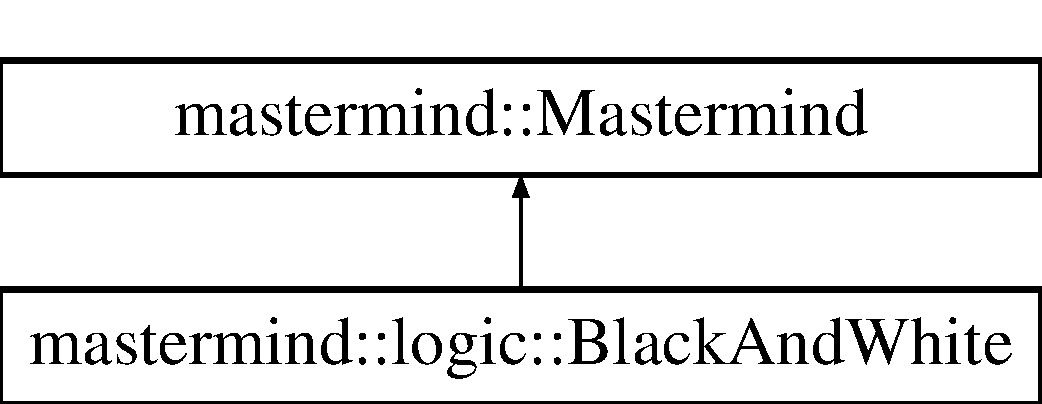
\includegraphics[height=2.000000cm]{classmastermind_1_1logic_1_1_black_and_white}
\end{center}
\end{figure}
\subsection*{Public Member Functions}
\begin{DoxyCompactItemize}
\item 
\hyperlink{classmastermind_1_1logic_1_1_black_and_white_a4dbd770b9f1ba3bef45ebba9fc01dcf4}{Black\+And\+White} (std\+::size\+\_\+t blacks, std\+::size\+\_\+t whites)
\begin{DoxyCompactList}\small\item\em Create \hyperlink{classmastermind_1_1logic_1_1_black_and_white}{Black\+And\+White}. \end{DoxyCompactList}\item 
\hyperlink{classmastermind_1_1logic_1_1_black_and_white_af6fc312cb65dcb1cc53f6e75cf45861d}{Black\+And\+White} (std\+::list$<$ int $>$ \&sticks)
\begin{DoxyCompactList}\small\item\em Create \hyperlink{classmastermind_1_1logic_1_1_black_and_white}{Black\+And\+White}. \end{DoxyCompactList}\item 
virtual std\+::wstring \hyperlink{classmastermind_1_1logic_1_1_black_and_white_aaa1108efb71702c9cdf6ac9a9ad4a0c9}{to\+String} () const
\begin{DoxyCompactList}\small\item\em Get string representation. \end{DoxyCompactList}\item 
std\+::wstring \hyperlink{classmastermind_1_1logic_1_1_black_and_white_a38779882fc72d356a660026e047eafb9}{to\+String\+Without\+Description} () const
\begin{DoxyCompactList}\small\item\em Get string representation. \end{DoxyCompactList}\item 
bool \hyperlink{classmastermind_1_1logic_1_1_black_and_white_ade7da8e1b846896a978f619b9689a7cb}{operator==} (const \hyperlink{classmastermind_1_1logic_1_1_black_and_white}{Black\+And\+White} \&rhs) const
\begin{DoxyCompactList}\small\item\em Test equality. \end{DoxyCompactList}\item 
bool \hyperlink{classmastermind_1_1logic_1_1_black_and_white_a8d622959805faeb3f63b0342667b58f7}{operator!=} (const \hyperlink{classmastermind_1_1logic_1_1_black_and_white}{Black\+And\+White} \&rhs) const
\begin{DoxyCompactList}\small\item\em Test inequality. \end{DoxyCompactList}\item 
std\+::size\+\_\+t \hyperlink{classmastermind_1_1logic_1_1_black_and_white_a85a1deac6d5cae64adce52aee8604fb0}{get\+White} () const
\begin{DoxyCompactList}\small\item\em Get amount of white sticks. \end{DoxyCompactList}\item 
std\+::size\+\_\+t \hyperlink{classmastermind_1_1logic_1_1_black_and_white_a5215b8ea947ec23c323448b46ba9e897}{get\+Black} () const
\begin{DoxyCompactList}\small\item\em Get amount of black sticks. \end{DoxyCompactList}\end{DoxyCompactItemize}
\subsection*{Static Public Attributes}
\begin{DoxyCompactItemize}
\item 
static const \hyperlink{classmastermind_1_1logic_1_1_black_and_white}{Black\+And\+White} \hyperlink{classmastermind_1_1logic_1_1_black_and_white_a9c0ca1063cd6e8d41b0d87d510de33f5}{W\+I\+N\+\_\+\+S\+T\+I\+C\+KS} = \hyperlink{classmastermind_1_1logic_1_1_black_and_white}{Black\+And\+White}(\hyperlink{classmastermind_1_1_mastermind_ad4cfc8127641ff8dfe89d65ae232331c}{S\+L\+O\+T\+\_\+\+C\+O\+U\+NT}, 0)
\begin{DoxyCompactList}\small\item\em Stick combination for a win. All black, zero white. \end{DoxyCompactList}\end{DoxyCompactItemize}
\subsection*{Additional Inherited Members}


\subsection{Detailed Description}
Representation for evaluation sticks. Black sticks show color and position right. White sticks show color right but wrong position. 

\subsection{Constructor \& Destructor Documentation}
\hypertarget{classmastermind_1_1logic_1_1_black_and_white_a4dbd770b9f1ba3bef45ebba9fc01dcf4}{}\label{classmastermind_1_1logic_1_1_black_and_white_a4dbd770b9f1ba3bef45ebba9fc01dcf4} 
\index{mastermind\+::logic\+::\+Black\+And\+White@{mastermind\+::logic\+::\+Black\+And\+White}!Black\+And\+White@{Black\+And\+White}}
\index{Black\+And\+White@{Black\+And\+White}!mastermind\+::logic\+::\+Black\+And\+White@{mastermind\+::logic\+::\+Black\+And\+White}}
\subsubsection{\texorpdfstring{Black\+And\+White()}{BlackAndWhite()}\hspace{0.1cm}{\footnotesize\ttfamily [1/2]}}
{\footnotesize\ttfamily mastermind\+::logic\+::\+Black\+And\+White\+::\+Black\+And\+White (\begin{DoxyParamCaption}\item[{std\+::size\+\_\+t}]{blacks,  }\item[{std\+::size\+\_\+t}]{whites }\end{DoxyParamCaption})}



Create \hyperlink{classmastermind_1_1logic_1_1_black_and_white}{Black\+And\+White}. 


\begin{DoxyParams}{Parameters}
{\em blacks} & amount of black sticks \\
\hline
{\em whites} & amount of white sticks \\
\hline
\end{DoxyParams}
\hypertarget{classmastermind_1_1logic_1_1_black_and_white_af6fc312cb65dcb1cc53f6e75cf45861d}{}\label{classmastermind_1_1logic_1_1_black_and_white_af6fc312cb65dcb1cc53f6e75cf45861d} 
\index{mastermind\+::logic\+::\+Black\+And\+White@{mastermind\+::logic\+::\+Black\+And\+White}!Black\+And\+White@{Black\+And\+White}}
\index{Black\+And\+White@{Black\+And\+White}!mastermind\+::logic\+::\+Black\+And\+White@{mastermind\+::logic\+::\+Black\+And\+White}}
\subsubsection{\texorpdfstring{Black\+And\+White()}{BlackAndWhite()}\hspace{0.1cm}{\footnotesize\ttfamily [2/2]}}
{\footnotesize\ttfamily mastermind\+::logic\+::\+Black\+And\+White\+::\+Black\+And\+White (\begin{DoxyParamCaption}\item[{std\+::list$<$ int $>$ \&}]{sticks }\end{DoxyParamCaption})}



Create \hyperlink{classmastermind_1_1logic_1_1_black_and_white}{Black\+And\+White}. 


\begin{DoxyParams}{Parameters}
{\em sticks} & list with {\ttfamily size == 2}, first is blacks and second is whites \\
\hline
\end{DoxyParams}


\subsection{Member Function Documentation}
\hypertarget{classmastermind_1_1logic_1_1_black_and_white_a5215b8ea947ec23c323448b46ba9e897}{}\label{classmastermind_1_1logic_1_1_black_and_white_a5215b8ea947ec23c323448b46ba9e897} 
\index{mastermind\+::logic\+::\+Black\+And\+White@{mastermind\+::logic\+::\+Black\+And\+White}!get\+Black@{get\+Black}}
\index{get\+Black@{get\+Black}!mastermind\+::logic\+::\+Black\+And\+White@{mastermind\+::logic\+::\+Black\+And\+White}}
\subsubsection{\texorpdfstring{get\+Black()}{getBlack()}}
{\footnotesize\ttfamily std\+::size\+\_\+t mastermind\+::logic\+::\+Black\+And\+White\+::get\+Black (\begin{DoxyParamCaption}{ }\end{DoxyParamCaption}) const}



Get amount of black sticks. 

\begin{DoxyReturn}{Returns}
amount of black sticks. 
\end{DoxyReturn}
\hypertarget{classmastermind_1_1logic_1_1_black_and_white_a85a1deac6d5cae64adce52aee8604fb0}{}\label{classmastermind_1_1logic_1_1_black_and_white_a85a1deac6d5cae64adce52aee8604fb0} 
\index{mastermind\+::logic\+::\+Black\+And\+White@{mastermind\+::logic\+::\+Black\+And\+White}!get\+White@{get\+White}}
\index{get\+White@{get\+White}!mastermind\+::logic\+::\+Black\+And\+White@{mastermind\+::logic\+::\+Black\+And\+White}}
\subsubsection{\texorpdfstring{get\+White()}{getWhite()}}
{\footnotesize\ttfamily std\+::size\+\_\+t mastermind\+::logic\+::\+Black\+And\+White\+::get\+White (\begin{DoxyParamCaption}{ }\end{DoxyParamCaption}) const}



Get amount of white sticks. 

\begin{DoxyReturn}{Returns}
amount of white sticks 
\end{DoxyReturn}
\hypertarget{classmastermind_1_1logic_1_1_black_and_white_a8d622959805faeb3f63b0342667b58f7}{}\label{classmastermind_1_1logic_1_1_black_and_white_a8d622959805faeb3f63b0342667b58f7} 
\index{mastermind\+::logic\+::\+Black\+And\+White@{mastermind\+::logic\+::\+Black\+And\+White}!operator"!=@{operator"!=}}
\index{operator"!=@{operator"!=}!mastermind\+::logic\+::\+Black\+And\+White@{mastermind\+::logic\+::\+Black\+And\+White}}
\subsubsection{\texorpdfstring{operator"!=()}{operator!=()}}
{\footnotesize\ttfamily bool mastermind\+::logic\+::\+Black\+And\+White\+::operator!= (\begin{DoxyParamCaption}\item[{const \hyperlink{classmastermind_1_1logic_1_1_black_and_white}{Black\+And\+White} \&}]{rhs }\end{DoxyParamCaption}) const}



Test inequality. 


\begin{DoxyParams}{Parameters}
{\em rhs} & the right hand side \hyperlink{classmastermind_1_1logic_1_1_black_and_white}{Black\+And\+White} \\
\hline
\end{DoxyParams}
\begin{DoxyReturn}{Returns}
{\ttfamily true} if {\ttfamily !(a == b)} 
\end{DoxyReturn}
\hypertarget{classmastermind_1_1logic_1_1_black_and_white_ade7da8e1b846896a978f619b9689a7cb}{}\label{classmastermind_1_1logic_1_1_black_and_white_ade7da8e1b846896a978f619b9689a7cb} 
\index{mastermind\+::logic\+::\+Black\+And\+White@{mastermind\+::logic\+::\+Black\+And\+White}!operator==@{operator==}}
\index{operator==@{operator==}!mastermind\+::logic\+::\+Black\+And\+White@{mastermind\+::logic\+::\+Black\+And\+White}}
\subsubsection{\texorpdfstring{operator==()}{operator==()}}
{\footnotesize\ttfamily bool mastermind\+::logic\+::\+Black\+And\+White\+::operator== (\begin{DoxyParamCaption}\item[{const \hyperlink{classmastermind_1_1logic_1_1_black_and_white}{Black\+And\+White} \&}]{rhs }\end{DoxyParamCaption}) const}



Test equality. 


\begin{DoxyParams}{Parameters}
{\em rhs} & the right hand side \hyperlink{classmastermind_1_1logic_1_1_black_and_white}{Black\+And\+White} \\
\hline
\end{DoxyParams}
\begin{DoxyReturn}{Returns}
{\ttfamily true} if amount of white left and right is equal and amount of black left and right is equal. 
\end{DoxyReturn}
\hypertarget{classmastermind_1_1logic_1_1_black_and_white_aaa1108efb71702c9cdf6ac9a9ad4a0c9}{}\label{classmastermind_1_1logic_1_1_black_and_white_aaa1108efb71702c9cdf6ac9a9ad4a0c9} 
\index{mastermind\+::logic\+::\+Black\+And\+White@{mastermind\+::logic\+::\+Black\+And\+White}!to\+String@{to\+String}}
\index{to\+String@{to\+String}!mastermind\+::logic\+::\+Black\+And\+White@{mastermind\+::logic\+::\+Black\+And\+White}}
\subsubsection{\texorpdfstring{to\+String()}{toString()}}
{\footnotesize\ttfamily std\+::wstring mastermind\+::logic\+::\+Black\+And\+White\+::to\+String (\begin{DoxyParamCaption}{ }\end{DoxyParamCaption}) const\hspace{0.3cm}{\ttfamily [virtual]}}



Get string representation. 

\begin{DoxyReturn}{Returns}
string in format \char`\"{}black\+: \%i white\+: \%i\char`\"{} 
\end{DoxyReturn}
\hypertarget{classmastermind_1_1logic_1_1_black_and_white_a38779882fc72d356a660026e047eafb9}{}\label{classmastermind_1_1logic_1_1_black_and_white_a38779882fc72d356a660026e047eafb9} 
\index{mastermind\+::logic\+::\+Black\+And\+White@{mastermind\+::logic\+::\+Black\+And\+White}!to\+String\+Without\+Description@{to\+String\+Without\+Description}}
\index{to\+String\+Without\+Description@{to\+String\+Without\+Description}!mastermind\+::logic\+::\+Black\+And\+White@{mastermind\+::logic\+::\+Black\+And\+White}}
\subsubsection{\texorpdfstring{to\+String\+Without\+Description()}{toStringWithoutDescription()}}
{\footnotesize\ttfamily std\+::wstring mastermind\+::logic\+::\+Black\+And\+White\+::to\+String\+Without\+Description (\begin{DoxyParamCaption}{ }\end{DoxyParamCaption}) const}



Get string representation. 

\begin{DoxyReturn}{Returns}
string in format \char`\"{}\%i \%i\char`\"{} 
\end{DoxyReturn}


\subsection{Member Data Documentation}
\hypertarget{classmastermind_1_1logic_1_1_black_and_white_a9c0ca1063cd6e8d41b0d87d510de33f5}{}\label{classmastermind_1_1logic_1_1_black_and_white_a9c0ca1063cd6e8d41b0d87d510de33f5} 
\index{mastermind\+::logic\+::\+Black\+And\+White@{mastermind\+::logic\+::\+Black\+And\+White}!W\+I\+N\+\_\+\+S\+T\+I\+C\+KS@{W\+I\+N\+\_\+\+S\+T\+I\+C\+KS}}
\index{W\+I\+N\+\_\+\+S\+T\+I\+C\+KS@{W\+I\+N\+\_\+\+S\+T\+I\+C\+KS}!mastermind\+::logic\+::\+Black\+And\+White@{mastermind\+::logic\+::\+Black\+And\+White}}
\subsubsection{\texorpdfstring{W\+I\+N\+\_\+\+S\+T\+I\+C\+KS}{WIN\_STICKS}}
{\footnotesize\ttfamily const \hyperlink{classmastermind_1_1logic_1_1_black_and_white}{Black\+And\+White} mastermind\+::logic\+::\+Black\+And\+White\+::\+W\+I\+N\+\_\+\+S\+T\+I\+C\+KS = \hyperlink{classmastermind_1_1logic_1_1_black_and_white}{Black\+And\+White}(\hyperlink{classmastermind_1_1_mastermind_ad4cfc8127641ff8dfe89d65ae232331c}{S\+L\+O\+T\+\_\+\+C\+O\+U\+NT}, 0)\hspace{0.3cm}{\ttfamily [static]}}



Stick combination for a win. All black, zero white. 



The documentation for this class was generated from the following files\+:\begin{DoxyCompactItemize}
\item 
Mastermind\+C\+P\+P\+D\+L\+L/\hyperlink{_black_and_white_8h}{Black\+And\+White.\+h}\item 
Mastermind\+C\+P\+P\+D\+L\+L/\hyperlink{_black_and_white_8cpp}{Black\+And\+White.\+cpp}\end{DoxyCompactItemize}

\hypertarget{classmastermind_1_1logic_1_1_color}{}\section{mastermind\+:\+:logic\+:\+:Color Class Reference}
\label{classmastermind_1_1logic_1_1_color}\index{mastermind\+::logic\+::\+Color@{mastermind\+::logic\+::\+Color}}


A color representation.  




{\ttfamily \#include $<$Color.\+h$>$}

Inheritance diagram for mastermind\+:\+:logic\+:\+:Color\+:\begin{figure}[H]
\begin{center}
\leavevmode
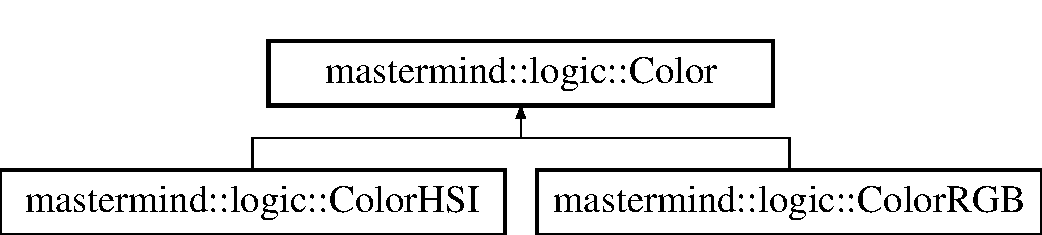
\includegraphics[height=2.000000cm]{classmastermind_1_1logic_1_1_color}
\end{center}
\end{figure}
\subsection*{Public Member Functions}
\begin{DoxyCompactItemize}
\item 
\hyperlink{classmastermind_1_1logic_1_1_color_a9f3666f78ecc894138a724d57ec271b2}{Color} ()
\item 
\hyperlink{classmastermind_1_1logic_1_1_color_ac1e72fd3f7927c56259c3bcce1b2b248}{Color} (std\+::wstring \hyperlink{classmastermind_1_1logic_1_1_color_aa086b665d9a43db3acbd43ed7f4d31ba}{name})
\item 
virtual \hyperlink{classmastermind_1_1logic_1_1_color_ab8ea1579c6a52d47a0dfeb7eb524e147}{$\sim$\+Color} ()
\item 
virtual std\+::wstring \hyperlink{classmastermind_1_1logic_1_1_color_ab911e1ca9d820b7d97c8e014ff75bc49}{to\+String} () const override
\begin{DoxyCompactList}\small\item\em String representation of this \hyperlink{classmastermind_1_1logic_1_1_color}{Color}. \end{DoxyCompactList}\item 
std\+::wstring \hyperlink{classmastermind_1_1logic_1_1_color_a4a591bc7e973ba8a224d63d32929daf1}{get\+Name} () const
\begin{DoxyCompactList}\small\item\em Get name of this color. \end{DoxyCompactList}\end{DoxyCompactItemize}
\subsection*{Static Public Member Functions}
\begin{DoxyCompactItemize}
\item 
static \hyperlink{classmastermind_1_1logic_1_1_color_r_g_b}{Color\+R\+GB} $\ast$ \hyperlink{classmastermind_1_1logic_1_1_color_abdfea9c0cb5c82afd84c96422a520655}{hsi\+To\+R\+GB} (const \hyperlink{classmastermind_1_1logic_1_1_color_h_s_i}{Color\+H\+SI} \&hsi)
\item 
static \hyperlink{classmastermind_1_1logic_1_1_color_h_s_i}{Color\+H\+SI} $\ast$ \hyperlink{classmastermind_1_1logic_1_1_color_a8a5e0010371827813a79b778af116bdb}{rgb\+To\+H\+SI} (const \hyperlink{classmastermind_1_1logic_1_1_color_r_g_b}{Color\+R\+GB} \&rgb)
\end{DoxyCompactItemize}
\subsection*{Private Attributes}
\begin{DoxyCompactItemize}
\item 
const std\+::wstring \hyperlink{classmastermind_1_1logic_1_1_color_aa086b665d9a43db3acbd43ed7f4d31ba}{name}
\begin{DoxyCompactList}\small\item\em Name of this color. \end{DoxyCompactList}\end{DoxyCompactItemize}


\subsection{Detailed Description}
A color representation. 

\subsection{Constructor \& Destructor Documentation}
\hypertarget{classmastermind_1_1logic_1_1_color_a9f3666f78ecc894138a724d57ec271b2}{}\label{classmastermind_1_1logic_1_1_color_a9f3666f78ecc894138a724d57ec271b2} 
\index{mastermind\+::logic\+::\+Color@{mastermind\+::logic\+::\+Color}!Color@{Color}}
\index{Color@{Color}!mastermind\+::logic\+::\+Color@{mastermind\+::logic\+::\+Color}}
\subsubsection{\texorpdfstring{Color()}{Color()}\hspace{0.1cm}{\footnotesize\ttfamily [1/2]}}
{\footnotesize\ttfamily mastermind\+::logic\+::\+Color\+::\+Color (\begin{DoxyParamCaption}{ }\end{DoxyParamCaption})}

\hypertarget{classmastermind_1_1logic_1_1_color_ac1e72fd3f7927c56259c3bcce1b2b248}{}\label{classmastermind_1_1logic_1_1_color_ac1e72fd3f7927c56259c3bcce1b2b248} 
\index{mastermind\+::logic\+::\+Color@{mastermind\+::logic\+::\+Color}!Color@{Color}}
\index{Color@{Color}!mastermind\+::logic\+::\+Color@{mastermind\+::logic\+::\+Color}}
\subsubsection{\texorpdfstring{Color()}{Color()}\hspace{0.1cm}{\footnotesize\ttfamily [2/2]}}
{\footnotesize\ttfamily mastermind\+::logic\+::\+Color\+::\+Color (\begin{DoxyParamCaption}\item[{std\+::wstring}]{name }\end{DoxyParamCaption})}

\hypertarget{classmastermind_1_1logic_1_1_color_ab8ea1579c6a52d47a0dfeb7eb524e147}{}\label{classmastermind_1_1logic_1_1_color_ab8ea1579c6a52d47a0dfeb7eb524e147} 
\index{mastermind\+::logic\+::\+Color@{mastermind\+::logic\+::\+Color}!````~Color@{$\sim$\+Color}}
\index{````~Color@{$\sim$\+Color}!mastermind\+::logic\+::\+Color@{mastermind\+::logic\+::\+Color}}
\subsubsection{\texorpdfstring{$\sim$\+Color()}{~Color()}}
{\footnotesize\ttfamily virtual mastermind\+::logic\+::\+Color\+::$\sim$\+Color (\begin{DoxyParamCaption}{ }\end{DoxyParamCaption})\hspace{0.3cm}{\ttfamily [inline]}, {\ttfamily [virtual]}}



\subsection{Member Function Documentation}
\hypertarget{classmastermind_1_1logic_1_1_color_a4a591bc7e973ba8a224d63d32929daf1}{}\label{classmastermind_1_1logic_1_1_color_a4a591bc7e973ba8a224d63d32929daf1} 
\index{mastermind\+::logic\+::\+Color@{mastermind\+::logic\+::\+Color}!get\+Name@{get\+Name}}
\index{get\+Name@{get\+Name}!mastermind\+::logic\+::\+Color@{mastermind\+::logic\+::\+Color}}
\subsubsection{\texorpdfstring{get\+Name()}{getName()}}
{\footnotesize\ttfamily std\+::wstring mastermind\+::logic\+::\+Color\+::get\+Name (\begin{DoxyParamCaption}{ }\end{DoxyParamCaption}) const}



Get name of this color. 

\begin{DoxyReturn}{Returns}
the name or {\ttfamily L\char`\"{}\char`\"{}} if no name was given 
\end{DoxyReturn}
\hypertarget{classmastermind_1_1logic_1_1_color_abdfea9c0cb5c82afd84c96422a520655}{}\label{classmastermind_1_1logic_1_1_color_abdfea9c0cb5c82afd84c96422a520655} 
\index{mastermind\+::logic\+::\+Color@{mastermind\+::logic\+::\+Color}!hsi\+To\+R\+GB@{hsi\+To\+R\+GB}}
\index{hsi\+To\+R\+GB@{hsi\+To\+R\+GB}!mastermind\+::logic\+::\+Color@{mastermind\+::logic\+::\+Color}}
\subsubsection{\texorpdfstring{hsi\+To\+R\+G\+B()}{hsiToRGB()}}
{\footnotesize\ttfamily \hyperlink{classmastermind_1_1logic_1_1_color_r_g_b}{Color\+R\+GB} $\ast$ mastermind\+::logic\+::\+Color\+::hsi\+To\+R\+GB (\begin{DoxyParamCaption}\item[{const \hyperlink{classmastermind_1_1logic_1_1_color_h_s_i}{Color\+H\+SI} \&}]{hsi }\end{DoxyParamCaption})\hspace{0.3cm}{\ttfamily [static]}}

Get R\+GB color from H\+SI color. 
\begin{DoxyParams}{Parameters}
{\em hsi} & the H\+SI color \\
\hline
\end{DoxyParams}
\begin{DoxyReturn}{Returns}
the resulting R\+GB color 
\end{DoxyReturn}
\hypertarget{classmastermind_1_1logic_1_1_color_a8a5e0010371827813a79b778af116bdb}{}\label{classmastermind_1_1logic_1_1_color_a8a5e0010371827813a79b778af116bdb} 
\index{mastermind\+::logic\+::\+Color@{mastermind\+::logic\+::\+Color}!rgb\+To\+H\+SI@{rgb\+To\+H\+SI}}
\index{rgb\+To\+H\+SI@{rgb\+To\+H\+SI}!mastermind\+::logic\+::\+Color@{mastermind\+::logic\+::\+Color}}
\subsubsection{\texorpdfstring{rgb\+To\+H\+S\+I()}{rgbToHSI()}}
{\footnotesize\ttfamily \hyperlink{classmastermind_1_1logic_1_1_color_h_s_i}{Color\+H\+SI} $\ast$ mastermind\+::logic\+::\+Color\+::rgb\+To\+H\+SI (\begin{DoxyParamCaption}\item[{const \hyperlink{classmastermind_1_1logic_1_1_color_r_g_b}{Color\+R\+GB} \&}]{rgb }\end{DoxyParamCaption})\hspace{0.3cm}{\ttfamily [static]}}

Get H\+SI color from R\+GB color. 
\begin{DoxyParams}{Parameters}
{\em rgb} & the R\+GB color. \\
\hline
\end{DoxyParams}
\begin{DoxyReturn}{Returns}
the resulting H\+SI color 
\end{DoxyReturn}
\hypertarget{classmastermind_1_1logic_1_1_color_ab911e1ca9d820b7d97c8e014ff75bc49}{}\label{classmastermind_1_1logic_1_1_color_ab911e1ca9d820b7d97c8e014ff75bc49} 
\index{mastermind\+::logic\+::\+Color@{mastermind\+::logic\+::\+Color}!to\+String@{to\+String}}
\index{to\+String@{to\+String}!mastermind\+::logic\+::\+Color@{mastermind\+::logic\+::\+Color}}
\subsubsection{\texorpdfstring{to\+String()}{toString()}}
{\footnotesize\ttfamily virtual std\+::wstring mastermind\+::logic\+::\+Color\+::to\+String (\begin{DoxyParamCaption}{ }\end{DoxyParamCaption}) const\hspace{0.3cm}{\ttfamily [pure virtual]}}



String representation of this \hyperlink{classmastermind_1_1logic_1_1_color}{Color}. 

\begin{DoxyReturn}{Returns}
string in form {\ttfamily L\char`\"{}(\+R,\+G,\+B)\char`\"{}} or {\ttfamily L\char`\"{}(\+H,\+S,\+I)\char`\"{}} 
\end{DoxyReturn}


Implemented in \hyperlink{classmastermind_1_1logic_1_1_color_r_g_b_ab80986e7ab151d26d47ad28d153a6a88}{mastermind\+::logic\+::\+Color\+R\+GB}, and \hyperlink{classmastermind_1_1logic_1_1_color_h_s_i_a2cba1eccd441e55eef75639c2cf9433c}{mastermind\+::logic\+::\+Color\+H\+SI}.



\subsection{Member Data Documentation}
\hypertarget{classmastermind_1_1logic_1_1_color_aa086b665d9a43db3acbd43ed7f4d31ba}{}\label{classmastermind_1_1logic_1_1_color_aa086b665d9a43db3acbd43ed7f4d31ba} 
\index{mastermind\+::logic\+::\+Color@{mastermind\+::logic\+::\+Color}!name@{name}}
\index{name@{name}!mastermind\+::logic\+::\+Color@{mastermind\+::logic\+::\+Color}}
\subsubsection{\texorpdfstring{name}{name}}
{\footnotesize\ttfamily const std\+::wstring mastermind\+::logic\+::\+Color\+::name\hspace{0.3cm}{\ttfamily [private]}}



Name of this color. 



The documentation for this class was generated from the following files\+:\begin{DoxyCompactItemize}
\item 
Mastermind\+C\+P\+P\+D\+L\+L/\hyperlink{_color_8h}{Color.\+h}\item 
Mastermind\+C\+P\+P\+D\+L\+L/\hyperlink{_color_8cpp}{Color.\+cpp}\end{DoxyCompactItemize}

\hypertarget{classmastermind_1_1logic_1_1_color_code}{}\section{mastermind\+:\+:logic\+:\+:Color\+Code Class Reference}
\label{classmastermind_1_1logic_1_1_color_code}\index{mastermind\+::logic\+::\+Color\+Code@{mastermind\+::logic\+::\+Color\+Code}}


Represents one line of the game board.  




{\ttfamily \#include $<$Color\+Code.\+h$>$}

\subsection*{Public Member Functions}
\begin{DoxyCompactItemize}
\item 
\hyperlink{classmastermind_1_1logic_1_1_color_code_a9bc91c2e878553c2e7a5b0821b76c525}{Color\+Code} (std\+::vector$<$ \hyperlink{namespacemastermind_1_1logic_aab4e2166db8e8e5dcbed785c7927eca1}{color\+\_\+t} $>$ \&col)
\begin{DoxyCompactList}\small\item\em Create a \hyperlink{classmastermind_1_1logic_1_1_color_code}{Color\+Code}. \end{DoxyCompactList}\item 
\hyperlink{classmastermind_1_1logic_1_1_color_code_ab4f174ea13758a5328f23daf26d8d61f}{Color\+Code} (size\+\_\+t size, \hyperlink{namespacemastermind_1_1logic_aab4e2166db8e8e5dcbed785c7927eca1}{color\+\_\+t} col\mbox{[}$\,$\mbox{]})
\begin{DoxyCompactList}\small\item\em Create a \hyperlink{classmastermind_1_1logic_1_1_color_code}{Color\+Code}. \end{DoxyCompactList}\item 
\hyperlink{classmastermind_1_1logic_1_1_color_code_ae407455b2aa672f8183cad6ec76bc848}{Color\+Code} (std\+::list$<$ \hyperlink{namespacemastermind_1_1logic_aab4e2166db8e8e5dcbed785c7927eca1}{color\+\_\+t} $\ast$$>$ \&list)
\begin{DoxyCompactList}\small\item\em Create a \hyperlink{classmastermind_1_1logic_1_1_color_code}{Color\+Code}. \end{DoxyCompactList}\item 
virtual \hyperlink{classmastermind_1_1logic_1_1_color_code_aee5e4a3d13fd9e2e2c69964fdffe04cf}{$\sim$\+Color\+Code} ()
\begin{DoxyCompactList}\small\item\em Destruct this. \end{DoxyCompactList}\item 
\hyperlink{namespacemastermind_1_1logic_aab4e2166db8e8e5dcbed785c7927eca1}{color\+\_\+t} \hyperlink{classmastermind_1_1logic_1_1_color_code_afe89e87be3e662db633bd88d1b5656cf}{get} (std\+::size\+\_\+t index)
\begin{DoxyCompactList}\small\item\em Get color at index. \end{DoxyCompactList}\item 
\hyperlink{namespacemastermind_1_1logic_aab4e2166db8e8e5dcbed785c7927eca1}{color\+\_\+t} \hyperlink{classmastermind_1_1logic_1_1_color_code_a74577852416c1438e6f1f43d4a9a21d2}{operator\mbox{[}$\,$\mbox{]}} (std\+::size\+\_\+t i) const
\begin{DoxyCompactList}\small\item\em Get color at index. \end{DoxyCompactList}\item 
bool \hyperlink{classmastermind_1_1logic_1_1_color_code_a2bb0b3f30f7a353348a7b73da5b47e19}{operator==} (const \hyperlink{classmastermind_1_1logic_1_1_color_code}{Color\+Code} \&rhs) const
\begin{DoxyCompactList}\small\item\em Test equality to other \hyperlink{classmastermind_1_1logic_1_1_color_code}{Color\+Code}. \end{DoxyCompactList}\item 
virtual std\+::wstring \hyperlink{classmastermind_1_1logic_1_1_color_code_a5d3903d505ecbd831d7e3776a0076c51}{to\+String} () const
\begin{DoxyCompactList}\small\item\em String representation of \hyperlink{classmastermind_1_1logic_1_1_color_code}{Color\+Code}. \end{DoxyCompactList}\end{DoxyCompactItemize}
\subsection*{Private Attributes}
\begin{DoxyCompactItemize}
\item 
std\+::vector$<$ \hyperlink{namespacemastermind_1_1logic_aab4e2166db8e8e5dcbed785c7927eca1}{color\+\_\+t} $>$ \hyperlink{classmastermind_1_1logic_1_1_color_code_a02a3b075035fe1fbc03140c745a30679}{colors}
\begin{DoxyCompactList}\small\item\em Colors in the line. \end{DoxyCompactList}\end{DoxyCompactItemize}


\subsection{Detailed Description}
Represents one line of the game board. 

\subsection{Constructor \& Destructor Documentation}
\hypertarget{classmastermind_1_1logic_1_1_color_code_a9bc91c2e878553c2e7a5b0821b76c525}{}\label{classmastermind_1_1logic_1_1_color_code_a9bc91c2e878553c2e7a5b0821b76c525} 
\index{mastermind\+::logic\+::\+Color\+Code@{mastermind\+::logic\+::\+Color\+Code}!Color\+Code@{Color\+Code}}
\index{Color\+Code@{Color\+Code}!mastermind\+::logic\+::\+Color\+Code@{mastermind\+::logic\+::\+Color\+Code}}
\subsubsection{\texorpdfstring{Color\+Code()}{ColorCode()}\hspace{0.1cm}{\footnotesize\ttfamily [1/3]}}
{\footnotesize\ttfamily mastermind\+::logic\+::\+Color\+Code\+::\+Color\+Code (\begin{DoxyParamCaption}\item[{std\+::vector$<$ \hyperlink{namespacemastermind_1_1logic_aab4e2166db8e8e5dcbed785c7927eca1}{color\+\_\+t} $>$ \&}]{col }\end{DoxyParamCaption})}



Create a \hyperlink{classmastermind_1_1logic_1_1_color_code}{Color\+Code}. 


\begin{DoxyParams}{Parameters}
{\em col} & columns as std\+::array \\
\hline
\end{DoxyParams}
\hypertarget{classmastermind_1_1logic_1_1_color_code_ab4f174ea13758a5328f23daf26d8d61f}{}\label{classmastermind_1_1logic_1_1_color_code_ab4f174ea13758a5328f23daf26d8d61f} 
\index{mastermind\+::logic\+::\+Color\+Code@{mastermind\+::logic\+::\+Color\+Code}!Color\+Code@{Color\+Code}}
\index{Color\+Code@{Color\+Code}!mastermind\+::logic\+::\+Color\+Code@{mastermind\+::logic\+::\+Color\+Code}}
\subsubsection{\texorpdfstring{Color\+Code()}{ColorCode()}\hspace{0.1cm}{\footnotesize\ttfamily [2/3]}}
{\footnotesize\ttfamily mastermind\+::logic\+::\+Color\+Code\+::\+Color\+Code (\begin{DoxyParamCaption}\item[{size\+\_\+t}]{size,  }\item[{\hyperlink{namespacemastermind_1_1logic_aab4e2166db8e8e5dcbed785c7927eca1}{color\+\_\+t}}]{col\mbox{[}$\,$\mbox{]} }\end{DoxyParamCaption})}



Create a \hyperlink{classmastermind_1_1logic_1_1_color_code}{Color\+Code}. 


\begin{DoxyParams}{Parameters}
{\em size} & size of array \\
\hline
{\em col} & columns as color\+\_\+t\mbox{[}\mbox{]} \\
\hline
\end{DoxyParams}
\hypertarget{classmastermind_1_1logic_1_1_color_code_ae407455b2aa672f8183cad6ec76bc848}{}\label{classmastermind_1_1logic_1_1_color_code_ae407455b2aa672f8183cad6ec76bc848} 
\index{mastermind\+::logic\+::\+Color\+Code@{mastermind\+::logic\+::\+Color\+Code}!Color\+Code@{Color\+Code}}
\index{Color\+Code@{Color\+Code}!mastermind\+::logic\+::\+Color\+Code@{mastermind\+::logic\+::\+Color\+Code}}
\subsubsection{\texorpdfstring{Color\+Code()}{ColorCode()}\hspace{0.1cm}{\footnotesize\ttfamily [3/3]}}
{\footnotesize\ttfamily mastermind\+::logic\+::\+Color\+Code\+::\+Color\+Code (\begin{DoxyParamCaption}\item[{std\+::list$<$ \hyperlink{namespacemastermind_1_1logic_aab4e2166db8e8e5dcbed785c7927eca1}{color\+\_\+t} $\ast$$>$ \&}]{list }\end{DoxyParamCaption})}



Create a \hyperlink{classmastermind_1_1logic_1_1_color_code}{Color\+Code}. 


\begin{DoxyParams}{Parameters}
{\em list} & columns as std\+::list \\
\hline
\end{DoxyParams}
\hypertarget{classmastermind_1_1logic_1_1_color_code_aee5e4a3d13fd9e2e2c69964fdffe04cf}{}\label{classmastermind_1_1logic_1_1_color_code_aee5e4a3d13fd9e2e2c69964fdffe04cf} 
\index{mastermind\+::logic\+::\+Color\+Code@{mastermind\+::logic\+::\+Color\+Code}!````~Color\+Code@{$\sim$\+Color\+Code}}
\index{````~Color\+Code@{$\sim$\+Color\+Code}!mastermind\+::logic\+::\+Color\+Code@{mastermind\+::logic\+::\+Color\+Code}}
\subsubsection{\texorpdfstring{$\sim$\+Color\+Code()}{~ColorCode()}}
{\footnotesize\ttfamily mastermind\+::logic\+::\+Color\+Code\+::$\sim$\+Color\+Code (\begin{DoxyParamCaption}{ }\end{DoxyParamCaption})\hspace{0.3cm}{\ttfamily [virtual]}}



Destruct this. 



\subsection{Member Function Documentation}
\hypertarget{classmastermind_1_1logic_1_1_color_code_afe89e87be3e662db633bd88d1b5656cf}{}\label{classmastermind_1_1logic_1_1_color_code_afe89e87be3e662db633bd88d1b5656cf} 
\index{mastermind\+::logic\+::\+Color\+Code@{mastermind\+::logic\+::\+Color\+Code}!get@{get}}
\index{get@{get}!mastermind\+::logic\+::\+Color\+Code@{mastermind\+::logic\+::\+Color\+Code}}
\subsubsection{\texorpdfstring{get()}{get()}}
{\footnotesize\ttfamily \hyperlink{namespacemastermind_1_1logic_aab4e2166db8e8e5dcbed785c7927eca1}{color\+\_\+t} mastermind\+::logic\+::\+Color\+Code\+::get (\begin{DoxyParamCaption}\item[{std\+::size\+\_\+t}]{index }\end{DoxyParamCaption})}



Get color at index. 


\begin{DoxyParams}{Parameters}
{\em index} & the index \\
\hline
\end{DoxyParams}
\begin{DoxyReturn}{Returns}
color at index 
\end{DoxyReturn}
\hypertarget{classmastermind_1_1logic_1_1_color_code_a2bb0b3f30f7a353348a7b73da5b47e19}{}\label{classmastermind_1_1logic_1_1_color_code_a2bb0b3f30f7a353348a7b73da5b47e19} 
\index{mastermind\+::logic\+::\+Color\+Code@{mastermind\+::logic\+::\+Color\+Code}!operator==@{operator==}}
\index{operator==@{operator==}!mastermind\+::logic\+::\+Color\+Code@{mastermind\+::logic\+::\+Color\+Code}}
\subsubsection{\texorpdfstring{operator==()}{operator==()}}
{\footnotesize\ttfamily bool mastermind\+::logic\+::\+Color\+Code\+::operator== (\begin{DoxyParamCaption}\item[{const \hyperlink{classmastermind_1_1logic_1_1_color_code}{Color\+Code} \&}]{rhs }\end{DoxyParamCaption}) const}



Test equality to other \hyperlink{classmastermind_1_1logic_1_1_color_code}{Color\+Code}. 


\begin{DoxyParams}{Parameters}
{\em rhs} & the other \hyperlink{classmastermind_1_1logic_1_1_color_code}{Color\+Code} \\
\hline
\end{DoxyParams}
\begin{DoxyReturn}{Returns}
{\ttfamily true} if colors and their positions are the same. 
\end{DoxyReturn}
\hypertarget{classmastermind_1_1logic_1_1_color_code_a74577852416c1438e6f1f43d4a9a21d2}{}\label{classmastermind_1_1logic_1_1_color_code_a74577852416c1438e6f1f43d4a9a21d2} 
\index{mastermind\+::logic\+::\+Color\+Code@{mastermind\+::logic\+::\+Color\+Code}!operator\mbox{[}\mbox{]}@{operator[]}}
\index{operator\mbox{[}\mbox{]}@{operator[]}!mastermind\+::logic\+::\+Color\+Code@{mastermind\+::logic\+::\+Color\+Code}}
\subsubsection{\texorpdfstring{operator[]()}{operator[]()}}
{\footnotesize\ttfamily \hyperlink{namespacemastermind_1_1logic_aab4e2166db8e8e5dcbed785c7927eca1}{color\+\_\+t} mastermind\+::logic\+::\+Color\+Code\+::operator\mbox{[}$\,$\mbox{]} (\begin{DoxyParamCaption}\item[{std\+::size\+\_\+t}]{i }\end{DoxyParamCaption}) const}



Get color at index. 


\begin{DoxyParams}{Parameters}
{\em i} & the index \\
\hline
\end{DoxyParams}
\begin{DoxyReturn}{Returns}
color at index 
\end{DoxyReturn}
\hypertarget{classmastermind_1_1logic_1_1_color_code_a5d3903d505ecbd831d7e3776a0076c51}{}\label{classmastermind_1_1logic_1_1_color_code_a5d3903d505ecbd831d7e3776a0076c51} 
\index{mastermind\+::logic\+::\+Color\+Code@{mastermind\+::logic\+::\+Color\+Code}!to\+String@{to\+String}}
\index{to\+String@{to\+String}!mastermind\+::logic\+::\+Color\+Code@{mastermind\+::logic\+::\+Color\+Code}}
\subsubsection{\texorpdfstring{to\+String()}{toString()}}
{\footnotesize\ttfamily std\+::wstring mastermind\+::logic\+::\+Color\+Code\+::to\+String (\begin{DoxyParamCaption}{ }\end{DoxyParamCaption}) const\hspace{0.3cm}{\ttfamily [virtual]}}



String representation of \hyperlink{classmastermind_1_1logic_1_1_color_code}{Color\+Code}. 

\begin{DoxyReturn}{Returns}
the string 
\end{DoxyReturn}


\subsection{Member Data Documentation}
\hypertarget{classmastermind_1_1logic_1_1_color_code_a02a3b075035fe1fbc03140c745a30679}{}\label{classmastermind_1_1logic_1_1_color_code_a02a3b075035fe1fbc03140c745a30679} 
\index{mastermind\+::logic\+::\+Color\+Code@{mastermind\+::logic\+::\+Color\+Code}!colors@{colors}}
\index{colors@{colors}!mastermind\+::logic\+::\+Color\+Code@{mastermind\+::logic\+::\+Color\+Code}}
\subsubsection{\texorpdfstring{colors}{colors}}
{\footnotesize\ttfamily std\+::vector$<$\hyperlink{namespacemastermind_1_1logic_aab4e2166db8e8e5dcbed785c7927eca1}{color\+\_\+t}$>$ mastermind\+::logic\+::\+Color\+Code\+::colors\hspace{0.3cm}{\ttfamily [private]}}



Colors in the line. 



The documentation for this class was generated from the following files\+:\begin{DoxyCompactItemize}
\item 
Mastermind\+C\+P\+P\+D\+L\+L/\hyperlink{_color_code_8h}{Color\+Code.\+h}\item 
Mastermind\+C\+P\+P\+D\+L\+L/\hyperlink{_color_code_8cpp}{Color\+Code.\+cpp}\end{DoxyCompactItemize}

\hypertarget{classmastermind_1_1logic_1_1_color_h_s_i}{}\section{mastermind\+:\+:logic\+:\+:Color\+H\+SI Class Reference}
\label{classmastermind_1_1logic_1_1_color_h_s_i}\index{mastermind\+::logic\+::\+Color\+H\+SI@{mastermind\+::logic\+::\+Color\+H\+SI}}


A R\+GB color representation. R\+GB values must be each \mbox{[}0..255\mbox{]}.  




{\ttfamily \#include $<$Color\+H\+S\+I.\+h$>$}

Inheritance diagram for mastermind\+:\+:logic\+:\+:Color\+H\+SI\+:\begin{figure}[H]
\begin{center}
\leavevmode
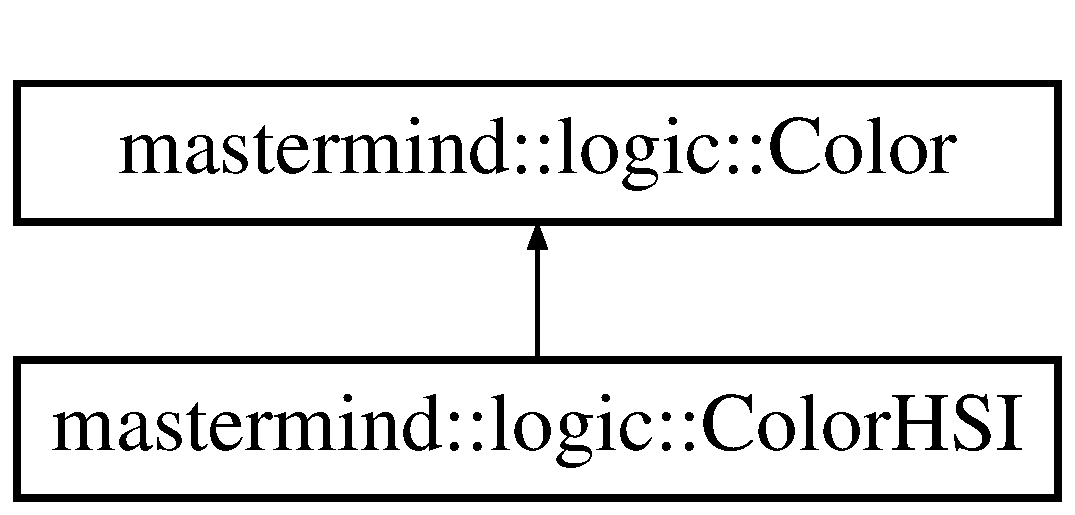
\includegraphics[height=2.000000cm]{classmastermind_1_1logic_1_1_color_h_s_i}
\end{center}
\end{figure}
\subsection*{Public Member Functions}
\begin{DoxyCompactItemize}
\item 
\hyperlink{classmastermind_1_1logic_1_1_color_h_s_i_a6e7465e8b360f30c35a6a27af15edfbe}{Color\+H\+SI} (double h, double s, double i)
\begin{DoxyCompactList}\small\item\em Create a H\+SI color. \end{DoxyCompactList}\item 
\hyperlink{classmastermind_1_1logic_1_1_color_h_s_i_a51e112e86cd7167eb5f2f7af72ba0a08}{Color\+H\+SI} (const \hyperlink{classmastermind_1_1logic_1_1_color_r_g_b}{Color\+R\+GB} \&color\+R\+GB)
\item 
double \hyperlink{classmastermind_1_1logic_1_1_color_h_s_i_ae22e195f505ccf77516944c3ea3062c9}{get\+Hue} () const
\begin{DoxyCompactList}\small\item\em Get hue value. \end{DoxyCompactList}\item 
double \hyperlink{classmastermind_1_1logic_1_1_color_h_s_i_a87b20bf4081e02865f648b1acc6e9b72}{get\+Saturation} () const
\begin{DoxyCompactList}\small\item\em Get saturation value. \end{DoxyCompactList}\item 
double \hyperlink{classmastermind_1_1logic_1_1_color_h_s_i_ab19f6d65c2b7a458de084738d017342a}{get\+Intensity} () const
\begin{DoxyCompactList}\small\item\em Get intensity value. \end{DoxyCompactList}\item 
double $\ast$ \hyperlink{classmastermind_1_1logic_1_1_color_h_s_i_aebf66c900b34e386b8ae72587f418ce9}{get\+H\+SI} () const
\begin{DoxyCompactList}\small\item\em Get R\+GB values as array. \end{DoxyCompactList}\item 
std\+::wstring \hyperlink{classmastermind_1_1logic_1_1_color_h_s_i_a2cba1eccd441e55eef75639c2cf9433c}{to\+String} () const override
\begin{DoxyCompactList}\small\item\em String representation of this \hyperlink{classmastermind_1_1logic_1_1_color}{Color}. \end{DoxyCompactList}\item 
bool \hyperlink{classmastermind_1_1logic_1_1_color_h_s_i_a63c8f95133b9c9e9936520e7cd2754fb}{operator==} (const \hyperlink{classmastermind_1_1logic_1_1_color_h_s_i}{Color\+H\+SI} \&rhs) const
\item 
bool \hyperlink{classmastermind_1_1logic_1_1_color_h_s_i_a32082591e8e68503c45e0516d7f62748}{operator!=} (const \hyperlink{classmastermind_1_1logic_1_1_color_h_s_i}{Color\+H\+SI} \&rhs) const
\end{DoxyCompactItemize}
\subsection*{Static Public Member Functions}
\begin{DoxyCompactItemize}
\item 
static double \hyperlink{classmastermind_1_1logic_1_1_color_h_s_i_a4364b93554d63622bea84177ae3b685a}{hue\+From\+R\+GB} (const \hyperlink{classmastermind_1_1logic_1_1_color_r_g_b}{Color\+R\+GB} \&rgb)
\item 
static double \hyperlink{classmastermind_1_1logic_1_1_color_h_s_i_aea09217f241f3548c3f45e6706596ada}{saturation\+From\+R\+GB} (const \hyperlink{classmastermind_1_1logic_1_1_color_r_g_b}{Color\+R\+GB} \&rgb)
\item 
static double \hyperlink{classmastermind_1_1logic_1_1_color_h_s_i_a921bf6e8d5e9d71d2823b2db2c9c84cb}{intensity\+From\+R\+GB} (const \hyperlink{classmastermind_1_1logic_1_1_color_r_g_b}{Color\+R\+GB} \&rgb)
\end{DoxyCompactItemize}
\subsection*{Private Attributes}
\begin{DoxyCompactItemize}
\item 
const double \hyperlink{classmastermind_1_1logic_1_1_color_h_s_i_a2b0bc5fa75a9c03ffe9ae4ebd9cc786c}{hue}
\begin{DoxyCompactList}\small\item\em Hue value. \end{DoxyCompactList}\item 
const double \hyperlink{classmastermind_1_1logic_1_1_color_h_s_i_a004dfa3a87c92f9890a7fc64b6b08c8f}{saturation}
\begin{DoxyCompactList}\small\item\em Saturation value. \end{DoxyCompactList}\item 
const double \hyperlink{classmastermind_1_1logic_1_1_color_h_s_i_acae1c5e74aae7a627bb1dbcd9f7ee521}{intensity}
\begin{DoxyCompactList}\small\item\em Intensity value. \end{DoxyCompactList}\end{DoxyCompactItemize}
\subsection*{Friends}
\begin{DoxyCompactItemize}
\item 
class \hyperlink{classmastermind_1_1logic_1_1_color_h_s_i_ae698553ee9010de895e223e73387f8dc}{Color\+R\+GB}
\end{DoxyCompactItemize}


\subsection{Detailed Description}
A R\+GB color representation. R\+GB values must be each \mbox{[}0..255\mbox{]}. 

\subsection{Constructor \& Destructor Documentation}
\hypertarget{classmastermind_1_1logic_1_1_color_h_s_i_a6e7465e8b360f30c35a6a27af15edfbe}{}\label{classmastermind_1_1logic_1_1_color_h_s_i_a6e7465e8b360f30c35a6a27af15edfbe} 
\index{mastermind\+::logic\+::\+Color\+H\+SI@{mastermind\+::logic\+::\+Color\+H\+SI}!Color\+H\+SI@{Color\+H\+SI}}
\index{Color\+H\+SI@{Color\+H\+SI}!mastermind\+::logic\+::\+Color\+H\+SI@{mastermind\+::logic\+::\+Color\+H\+SI}}
\subsubsection{\texorpdfstring{Color\+H\+S\+I()}{ColorHSI()}\hspace{0.1cm}{\footnotesize\ttfamily [1/2]}}
{\footnotesize\ttfamily mastermind\+::logic\+::\+Color\+H\+S\+I\+::\+Color\+H\+SI (\begin{DoxyParamCaption}\item[{double}]{h,  }\item[{double}]{s,  }\item[{double}]{i }\end{DoxyParamCaption})}



Create a H\+SI color. 


\begin{DoxyParams}{Parameters}
{\em h} & hue value, must be \mbox{[}0.\+0..360.\+0) \\
\hline
{\em s} & saturation value, must be \mbox{[}0.\+0..1.\+0\mbox{]} \\
\hline
{\em i} & intensity value, must be \mbox{[}0.\+0..1.\+0\mbox{]}\\
\hline
\end{DoxyParams}

\begin{DoxyExceptions}{Exceptions}
{\em std\+::invalid\+\_\+argument} & \\
\hline
\end{DoxyExceptions}
\hypertarget{classmastermind_1_1logic_1_1_color_h_s_i_a51e112e86cd7167eb5f2f7af72ba0a08}{}\label{classmastermind_1_1logic_1_1_color_h_s_i_a51e112e86cd7167eb5f2f7af72ba0a08} 
\index{mastermind\+::logic\+::\+Color\+H\+SI@{mastermind\+::logic\+::\+Color\+H\+SI}!Color\+H\+SI@{Color\+H\+SI}}
\index{Color\+H\+SI@{Color\+H\+SI}!mastermind\+::logic\+::\+Color\+H\+SI@{mastermind\+::logic\+::\+Color\+H\+SI}}
\subsubsection{\texorpdfstring{Color\+H\+S\+I()}{ColorHSI()}\hspace{0.1cm}{\footnotesize\ttfamily [2/2]}}
{\footnotesize\ttfamily mastermind\+::logic\+::\+Color\+H\+S\+I\+::\+Color\+H\+SI (\begin{DoxyParamCaption}\item[{const \hyperlink{classmastermind_1_1logic_1_1_color_r_g_b}{Color\+R\+GB} \&}]{color\+R\+GB }\end{DoxyParamCaption})}



\subsection{Member Function Documentation}
\hypertarget{classmastermind_1_1logic_1_1_color_h_s_i_aebf66c900b34e386b8ae72587f418ce9}{}\label{classmastermind_1_1logic_1_1_color_h_s_i_aebf66c900b34e386b8ae72587f418ce9} 
\index{mastermind\+::logic\+::\+Color\+H\+SI@{mastermind\+::logic\+::\+Color\+H\+SI}!get\+H\+SI@{get\+H\+SI}}
\index{get\+H\+SI@{get\+H\+SI}!mastermind\+::logic\+::\+Color\+H\+SI@{mastermind\+::logic\+::\+Color\+H\+SI}}
\subsubsection{\texorpdfstring{get\+H\+S\+I()}{getHSI()}}
{\footnotesize\ttfamily double $\ast$ mastermind\+::logic\+::\+Color\+H\+S\+I\+::get\+H\+SI (\begin{DoxyParamCaption}{ }\end{DoxyParamCaption}) const}



Get R\+GB values as array. 

\begin{DoxyReturn}{Returns}
array with H\+SI values 
\end{DoxyReturn}
\hypertarget{classmastermind_1_1logic_1_1_color_h_s_i_ae22e195f505ccf77516944c3ea3062c9}{}\label{classmastermind_1_1logic_1_1_color_h_s_i_ae22e195f505ccf77516944c3ea3062c9} 
\index{mastermind\+::logic\+::\+Color\+H\+SI@{mastermind\+::logic\+::\+Color\+H\+SI}!get\+Hue@{get\+Hue}}
\index{get\+Hue@{get\+Hue}!mastermind\+::logic\+::\+Color\+H\+SI@{mastermind\+::logic\+::\+Color\+H\+SI}}
\subsubsection{\texorpdfstring{get\+Hue()}{getHue()}}
{\footnotesize\ttfamily double mastermind\+::logic\+::\+Color\+H\+S\+I\+::get\+Hue (\begin{DoxyParamCaption}{ }\end{DoxyParamCaption}) const}



Get hue value. 

\begin{DoxyReturn}{Returns}
the hue value 
\end{DoxyReturn}
\hypertarget{classmastermind_1_1logic_1_1_color_h_s_i_ab19f6d65c2b7a458de084738d017342a}{}\label{classmastermind_1_1logic_1_1_color_h_s_i_ab19f6d65c2b7a458de084738d017342a} 
\index{mastermind\+::logic\+::\+Color\+H\+SI@{mastermind\+::logic\+::\+Color\+H\+SI}!get\+Intensity@{get\+Intensity}}
\index{get\+Intensity@{get\+Intensity}!mastermind\+::logic\+::\+Color\+H\+SI@{mastermind\+::logic\+::\+Color\+H\+SI}}
\subsubsection{\texorpdfstring{get\+Intensity()}{getIntensity()}}
{\footnotesize\ttfamily double mastermind\+::logic\+::\+Color\+H\+S\+I\+::get\+Intensity (\begin{DoxyParamCaption}{ }\end{DoxyParamCaption}) const}



Get intensity value. 

\begin{DoxyReturn}{Returns}
the intensity value 
\end{DoxyReturn}
\hypertarget{classmastermind_1_1logic_1_1_color_h_s_i_a87b20bf4081e02865f648b1acc6e9b72}{}\label{classmastermind_1_1logic_1_1_color_h_s_i_a87b20bf4081e02865f648b1acc6e9b72} 
\index{mastermind\+::logic\+::\+Color\+H\+SI@{mastermind\+::logic\+::\+Color\+H\+SI}!get\+Saturation@{get\+Saturation}}
\index{get\+Saturation@{get\+Saturation}!mastermind\+::logic\+::\+Color\+H\+SI@{mastermind\+::logic\+::\+Color\+H\+SI}}
\subsubsection{\texorpdfstring{get\+Saturation()}{getSaturation()}}
{\footnotesize\ttfamily double mastermind\+::logic\+::\+Color\+H\+S\+I\+::get\+Saturation (\begin{DoxyParamCaption}{ }\end{DoxyParamCaption}) const}



Get saturation value. 

\begin{DoxyReturn}{Returns}
the saturation value 
\end{DoxyReturn}
\hypertarget{classmastermind_1_1logic_1_1_color_h_s_i_a4364b93554d63622bea84177ae3b685a}{}\label{classmastermind_1_1logic_1_1_color_h_s_i_a4364b93554d63622bea84177ae3b685a} 
\index{mastermind\+::logic\+::\+Color\+H\+SI@{mastermind\+::logic\+::\+Color\+H\+SI}!hue\+From\+R\+GB@{hue\+From\+R\+GB}}
\index{hue\+From\+R\+GB@{hue\+From\+R\+GB}!mastermind\+::logic\+::\+Color\+H\+SI@{mastermind\+::logic\+::\+Color\+H\+SI}}
\subsubsection{\texorpdfstring{hue\+From\+R\+G\+B()}{hueFromRGB()}}
{\footnotesize\ttfamily double mastermind\+::logic\+::\+Color\+H\+S\+I\+::hue\+From\+R\+GB (\begin{DoxyParamCaption}\item[{const \hyperlink{classmastermind_1_1logic_1_1_color_r_g_b}{Color\+R\+GB} \&}]{rgb }\end{DoxyParamCaption})\hspace{0.3cm}{\ttfamily [static]}}

\hypertarget{classmastermind_1_1logic_1_1_color_h_s_i_a921bf6e8d5e9d71d2823b2db2c9c84cb}{}\label{classmastermind_1_1logic_1_1_color_h_s_i_a921bf6e8d5e9d71d2823b2db2c9c84cb} 
\index{mastermind\+::logic\+::\+Color\+H\+SI@{mastermind\+::logic\+::\+Color\+H\+SI}!intensity\+From\+R\+GB@{intensity\+From\+R\+GB}}
\index{intensity\+From\+R\+GB@{intensity\+From\+R\+GB}!mastermind\+::logic\+::\+Color\+H\+SI@{mastermind\+::logic\+::\+Color\+H\+SI}}
\subsubsection{\texorpdfstring{intensity\+From\+R\+G\+B()}{intensityFromRGB()}}
{\footnotesize\ttfamily double mastermind\+::logic\+::\+Color\+H\+S\+I\+::intensity\+From\+R\+GB (\begin{DoxyParamCaption}\item[{const \hyperlink{classmastermind_1_1logic_1_1_color_r_g_b}{Color\+R\+GB} \&}]{rgb }\end{DoxyParamCaption})\hspace{0.3cm}{\ttfamily [static]}}

\hypertarget{classmastermind_1_1logic_1_1_color_h_s_i_a32082591e8e68503c45e0516d7f62748}{}\label{classmastermind_1_1logic_1_1_color_h_s_i_a32082591e8e68503c45e0516d7f62748} 
\index{mastermind\+::logic\+::\+Color\+H\+SI@{mastermind\+::logic\+::\+Color\+H\+SI}!operator"!=@{operator"!=}}
\index{operator"!=@{operator"!=}!mastermind\+::logic\+::\+Color\+H\+SI@{mastermind\+::logic\+::\+Color\+H\+SI}}
\subsubsection{\texorpdfstring{operator"!=()}{operator!=()}}
{\footnotesize\ttfamily bool mastermind\+::logic\+::\+Color\+H\+S\+I\+::operator!= (\begin{DoxyParamCaption}\item[{const \hyperlink{classmastermind_1_1logic_1_1_color_h_s_i}{Color\+H\+SI} \&}]{rhs }\end{DoxyParamCaption}) const}

\hypertarget{classmastermind_1_1logic_1_1_color_h_s_i_a63c8f95133b9c9e9936520e7cd2754fb}{}\label{classmastermind_1_1logic_1_1_color_h_s_i_a63c8f95133b9c9e9936520e7cd2754fb} 
\index{mastermind\+::logic\+::\+Color\+H\+SI@{mastermind\+::logic\+::\+Color\+H\+SI}!operator==@{operator==}}
\index{operator==@{operator==}!mastermind\+::logic\+::\+Color\+H\+SI@{mastermind\+::logic\+::\+Color\+H\+SI}}
\subsubsection{\texorpdfstring{operator==()}{operator==()}}
{\footnotesize\ttfamily bool mastermind\+::logic\+::\+Color\+H\+S\+I\+::operator== (\begin{DoxyParamCaption}\item[{const \hyperlink{classmastermind_1_1logic_1_1_color_h_s_i}{Color\+H\+SI} \&}]{rhs }\end{DoxyParamCaption}) const}

\hypertarget{classmastermind_1_1logic_1_1_color_h_s_i_aea09217f241f3548c3f45e6706596ada}{}\label{classmastermind_1_1logic_1_1_color_h_s_i_aea09217f241f3548c3f45e6706596ada} 
\index{mastermind\+::logic\+::\+Color\+H\+SI@{mastermind\+::logic\+::\+Color\+H\+SI}!saturation\+From\+R\+GB@{saturation\+From\+R\+GB}}
\index{saturation\+From\+R\+GB@{saturation\+From\+R\+GB}!mastermind\+::logic\+::\+Color\+H\+SI@{mastermind\+::logic\+::\+Color\+H\+SI}}
\subsubsection{\texorpdfstring{saturation\+From\+R\+G\+B()}{saturationFromRGB()}}
{\footnotesize\ttfamily double mastermind\+::logic\+::\+Color\+H\+S\+I\+::saturation\+From\+R\+GB (\begin{DoxyParamCaption}\item[{const \hyperlink{classmastermind_1_1logic_1_1_color_r_g_b}{Color\+R\+GB} \&}]{rgb }\end{DoxyParamCaption})\hspace{0.3cm}{\ttfamily [static]}}

\hypertarget{classmastermind_1_1logic_1_1_color_h_s_i_a2cba1eccd441e55eef75639c2cf9433c}{}\label{classmastermind_1_1logic_1_1_color_h_s_i_a2cba1eccd441e55eef75639c2cf9433c} 
\index{mastermind\+::logic\+::\+Color\+H\+SI@{mastermind\+::logic\+::\+Color\+H\+SI}!to\+String@{to\+String}}
\index{to\+String@{to\+String}!mastermind\+::logic\+::\+Color\+H\+SI@{mastermind\+::logic\+::\+Color\+H\+SI}}
\subsubsection{\texorpdfstring{to\+String()}{toString()}}
{\footnotesize\ttfamily std\+::wstring mastermind\+::logic\+::\+Color\+H\+S\+I\+::to\+String (\begin{DoxyParamCaption}{ }\end{DoxyParamCaption}) const\hspace{0.3cm}{\ttfamily [override]}, {\ttfamily [virtual]}}



String representation of this \hyperlink{classmastermind_1_1logic_1_1_color}{Color}. 

\begin{DoxyReturn}{Returns}
string in form {\ttfamily L\char`\"{}(\+R,\+G,\+B)\char`\"{}} or {\ttfamily L\char`\"{}(\+H,\+S,\+I)\char`\"{}} 
\end{DoxyReturn}


Implements \hyperlink{classmastermind_1_1logic_1_1_color_ab911e1ca9d820b7d97c8e014ff75bc49}{mastermind\+::logic\+::\+Color}.



\subsection{Friends And Related Function Documentation}
\hypertarget{classmastermind_1_1logic_1_1_color_h_s_i_ae698553ee9010de895e223e73387f8dc}{}\label{classmastermind_1_1logic_1_1_color_h_s_i_ae698553ee9010de895e223e73387f8dc} 
\index{mastermind\+::logic\+::\+Color\+H\+SI@{mastermind\+::logic\+::\+Color\+H\+SI}!Color\+R\+GB@{Color\+R\+GB}}
\index{Color\+R\+GB@{Color\+R\+GB}!mastermind\+::logic\+::\+Color\+H\+SI@{mastermind\+::logic\+::\+Color\+H\+SI}}
\subsubsection{\texorpdfstring{Color\+R\+GB}{ColorRGB}}
{\footnotesize\ttfamily friend class \hyperlink{classmastermind_1_1logic_1_1_color_r_g_b}{Color\+R\+GB}\hspace{0.3cm}{\ttfamily [friend]}}



\subsection{Member Data Documentation}
\hypertarget{classmastermind_1_1logic_1_1_color_h_s_i_a2b0bc5fa75a9c03ffe9ae4ebd9cc786c}{}\label{classmastermind_1_1logic_1_1_color_h_s_i_a2b0bc5fa75a9c03ffe9ae4ebd9cc786c} 
\index{mastermind\+::logic\+::\+Color\+H\+SI@{mastermind\+::logic\+::\+Color\+H\+SI}!hue@{hue}}
\index{hue@{hue}!mastermind\+::logic\+::\+Color\+H\+SI@{mastermind\+::logic\+::\+Color\+H\+SI}}
\subsubsection{\texorpdfstring{hue}{hue}}
{\footnotesize\ttfamily const double mastermind\+::logic\+::\+Color\+H\+S\+I\+::hue\hspace{0.3cm}{\ttfamily [private]}}



Hue value. 

\hypertarget{classmastermind_1_1logic_1_1_color_h_s_i_acae1c5e74aae7a627bb1dbcd9f7ee521}{}\label{classmastermind_1_1logic_1_1_color_h_s_i_acae1c5e74aae7a627bb1dbcd9f7ee521} 
\index{mastermind\+::logic\+::\+Color\+H\+SI@{mastermind\+::logic\+::\+Color\+H\+SI}!intensity@{intensity}}
\index{intensity@{intensity}!mastermind\+::logic\+::\+Color\+H\+SI@{mastermind\+::logic\+::\+Color\+H\+SI}}
\subsubsection{\texorpdfstring{intensity}{intensity}}
{\footnotesize\ttfamily const double mastermind\+::logic\+::\+Color\+H\+S\+I\+::intensity\hspace{0.3cm}{\ttfamily [private]}}



Intensity value. 

\hypertarget{classmastermind_1_1logic_1_1_color_h_s_i_a004dfa3a87c92f9890a7fc64b6b08c8f}{}\label{classmastermind_1_1logic_1_1_color_h_s_i_a004dfa3a87c92f9890a7fc64b6b08c8f} 
\index{mastermind\+::logic\+::\+Color\+H\+SI@{mastermind\+::logic\+::\+Color\+H\+SI}!saturation@{saturation}}
\index{saturation@{saturation}!mastermind\+::logic\+::\+Color\+H\+SI@{mastermind\+::logic\+::\+Color\+H\+SI}}
\subsubsection{\texorpdfstring{saturation}{saturation}}
{\footnotesize\ttfamily const double mastermind\+::logic\+::\+Color\+H\+S\+I\+::saturation\hspace{0.3cm}{\ttfamily [private]}}



Saturation value. 



The documentation for this class was generated from the following files\+:\begin{DoxyCompactItemize}
\item 
Mastermind\+C\+P\+P\+D\+L\+L/\hyperlink{_color_h_s_i_8h}{Color\+H\+S\+I.\+h}\item 
Mastermind\+C\+P\+P\+D\+L\+L/\hyperlink{_color_h_s_i_8cpp}{Color\+H\+S\+I.\+cpp}\end{DoxyCompactItemize}

\hypertarget{classmastermind_1_1logic_1_1_color_r_g_b}{}\section{mastermind\+:\+:logic\+:\+:Color\+R\+GB Class Reference}
\label{classmastermind_1_1logic_1_1_color_r_g_b}\index{mastermind\+::logic\+::\+Color\+R\+GB@{mastermind\+::logic\+::\+Color\+R\+GB}}


A R\+GB color representation. R\+GB values must be each \mbox{[}0..255\mbox{]}.  




{\ttfamily \#include $<$Color\+R\+G\+B.\+h$>$}

Inheritance diagram for mastermind\+:\+:logic\+:\+:Color\+R\+GB\+:\begin{figure}[H]
\begin{center}
\leavevmode
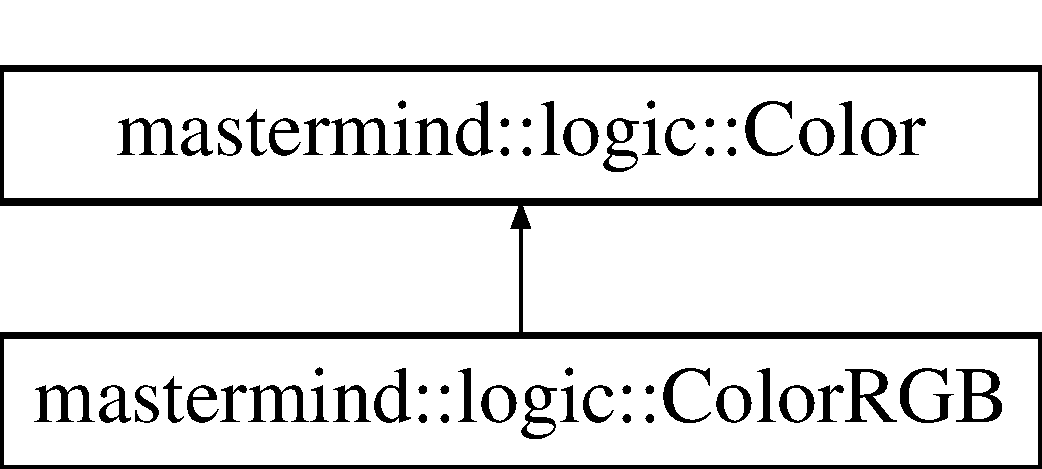
\includegraphics[height=2.000000cm]{classmastermind_1_1logic_1_1_color_r_g_b}
\end{center}
\end{figure}
\subsection*{Public Member Functions}
\begin{DoxyCompactItemize}
\item 
\hyperlink{classmastermind_1_1logic_1_1_color_r_g_b_a06ed69416fc73bb7456f281b32def4ea}{Color\+R\+GB} (std\+::wstring \hyperlink{classmastermind_1_1logic_1_1_color_aa086b665d9a43db3acbd43ed7f4d31ba}{name}, uint8\+\_\+t r, uint8\+\_\+t g, uint8\+\_\+t b)
\begin{DoxyCompactList}\small\item\em Create a R\+GB color. \end{DoxyCompactList}\item 
\hyperlink{classmastermind_1_1logic_1_1_color_r_g_b_aa8391f55de09ffdb14936ba1283e4a5b}{Color\+R\+GB} (uint8\+\_\+t r, uint8\+\_\+t g, uint8\+\_\+t b)
\begin{DoxyCompactList}\small\item\em Create a R\+GB color. \end{DoxyCompactList}\item 
uint8\+\_\+t \hyperlink{classmastermind_1_1logic_1_1_color_r_g_b_ace7e594445a112e54776f0e0a57e5478}{get\+Red} () const
\begin{DoxyCompactList}\small\item\em Get red value. \end{DoxyCompactList}\item 
uint8\+\_\+t \hyperlink{classmastermind_1_1logic_1_1_color_r_g_b_a4b4f9754ce5287b3b8abf61cbc84ad11}{get\+Green} () const
\begin{DoxyCompactList}\small\item\em Get green value. \end{DoxyCompactList}\item 
uint8\+\_\+t \hyperlink{classmastermind_1_1logic_1_1_color_r_g_b_a0838de88ff779b5640d47ad5130f379b}{get\+Blue} () const
\begin{DoxyCompactList}\small\item\em Get blue value. \end{DoxyCompactList}\item 
uint8\+\_\+t $\ast$ \hyperlink{classmastermind_1_1logic_1_1_color_r_g_b_a58bbc8f966399582307612db3da39acb}{get\+R\+GB} () const
\begin{DoxyCompactList}\small\item\em Get R\+GB values as array. \end{DoxyCompactList}\item 
std\+::wstring \hyperlink{classmastermind_1_1logic_1_1_color_r_g_b_ab80986e7ab151d26d47ad28d153a6a88}{to\+String} () const override
\begin{DoxyCompactList}\small\item\em String representation of this \hyperlink{classmastermind_1_1logic_1_1_color}{Color}. \end{DoxyCompactList}\item 
bool \hyperlink{classmastermind_1_1logic_1_1_color_r_g_b_abe96ac5c31537e3bafaa52d1eab98a2f}{operator==} (const \hyperlink{classmastermind_1_1logic_1_1_color_r_g_b}{Color\+R\+GB} \&rhs) const
\item 
bool \hyperlink{classmastermind_1_1logic_1_1_color_r_g_b_ab81f315c0d1bba56d40a1766b51b0273}{operator!=} (const \hyperlink{classmastermind_1_1logic_1_1_color_r_g_b}{Color\+R\+GB} \&rhs) const
\end{DoxyCompactItemize}
\subsection*{Private Attributes}
\begin{DoxyCompactItemize}
\item 
const uint8\+\_\+t \hyperlink{classmastermind_1_1logic_1_1_color_r_g_b_a8f9661c51195e67f2c22009805e6b3d2}{red}
\begin{DoxyCompactList}\small\item\em Red value. \end{DoxyCompactList}\item 
const uint8\+\_\+t \hyperlink{classmastermind_1_1logic_1_1_color_r_g_b_abcdd46578394ad832e79ccf2affdd51e}{green}
\begin{DoxyCompactList}\small\item\em Green value. \end{DoxyCompactList}\item 
const uint8\+\_\+t \hyperlink{classmastermind_1_1logic_1_1_color_r_g_b_a9bfa135c10da9636ed9c0c1310b50731}{blue}
\begin{DoxyCompactList}\small\item\em Blue value. \end{DoxyCompactList}\end{DoxyCompactItemize}
\subsection*{Friends}
\begin{DoxyCompactItemize}
\item 
class \hyperlink{classmastermind_1_1logic_1_1_color_r_g_b_ada143533c2a424e783d7a68a213d6537}{Color\+H\+SI}
\end{DoxyCompactItemize}
\subsection*{Additional Inherited Members}


\subsection{Detailed Description}
A R\+GB color representation. R\+GB values must be each \mbox{[}0..255\mbox{]}. 

\subsection{Constructor \& Destructor Documentation}
\hypertarget{classmastermind_1_1logic_1_1_color_r_g_b_a06ed69416fc73bb7456f281b32def4ea}{}\label{classmastermind_1_1logic_1_1_color_r_g_b_a06ed69416fc73bb7456f281b32def4ea} 
\index{mastermind\+::logic\+::\+Color\+R\+GB@{mastermind\+::logic\+::\+Color\+R\+GB}!Color\+R\+GB@{Color\+R\+GB}}
\index{Color\+R\+GB@{Color\+R\+GB}!mastermind\+::logic\+::\+Color\+R\+GB@{mastermind\+::logic\+::\+Color\+R\+GB}}
\subsubsection{\texorpdfstring{Color\+R\+G\+B()}{ColorRGB()}\hspace{0.1cm}{\footnotesize\ttfamily [1/2]}}
{\footnotesize\ttfamily mastermind\+::logic\+::\+Color\+R\+G\+B\+::\+Color\+R\+GB (\begin{DoxyParamCaption}\item[{std\+::wstring}]{name,  }\item[{uint8\+\_\+t}]{r,  }\item[{uint8\+\_\+t}]{g,  }\item[{uint8\+\_\+t}]{b }\end{DoxyParamCaption})}



Create a R\+GB color. 


\begin{DoxyParams}{Parameters}
{\em name} & name for this color \\
\hline
{\em r} & red value, must be \mbox{[}0..255\mbox{]} \\
\hline
{\em g} & green value, must be \mbox{[}0..255\mbox{]} \\
\hline
{\em b} & blue value, must be \mbox{[}0..255\mbox{]} \\
\hline
\end{DoxyParams}
\hypertarget{classmastermind_1_1logic_1_1_color_r_g_b_aa8391f55de09ffdb14936ba1283e4a5b}{}\label{classmastermind_1_1logic_1_1_color_r_g_b_aa8391f55de09ffdb14936ba1283e4a5b} 
\index{mastermind\+::logic\+::\+Color\+R\+GB@{mastermind\+::logic\+::\+Color\+R\+GB}!Color\+R\+GB@{Color\+R\+GB}}
\index{Color\+R\+GB@{Color\+R\+GB}!mastermind\+::logic\+::\+Color\+R\+GB@{mastermind\+::logic\+::\+Color\+R\+GB}}
\subsubsection{\texorpdfstring{Color\+R\+G\+B()}{ColorRGB()}\hspace{0.1cm}{\footnotesize\ttfamily [2/2]}}
{\footnotesize\ttfamily mastermind\+::logic\+::\+Color\+R\+G\+B\+::\+Color\+R\+GB (\begin{DoxyParamCaption}\item[{uint8\+\_\+t}]{r,  }\item[{uint8\+\_\+t}]{g,  }\item[{uint8\+\_\+t}]{b }\end{DoxyParamCaption})}



Create a R\+GB color. 


\begin{DoxyParams}{Parameters}
{\em r} & red value, must be \mbox{[}0..255\mbox{]} \\
\hline
{\em g} & green value, must be \mbox{[}0..255\mbox{]} \\
\hline
{\em b} & blue value, must be \mbox{[}0..255\mbox{]} \\
\hline
\end{DoxyParams}


\subsection{Member Function Documentation}
\hypertarget{classmastermind_1_1logic_1_1_color_r_g_b_a0838de88ff779b5640d47ad5130f379b}{}\label{classmastermind_1_1logic_1_1_color_r_g_b_a0838de88ff779b5640d47ad5130f379b} 
\index{mastermind\+::logic\+::\+Color\+R\+GB@{mastermind\+::logic\+::\+Color\+R\+GB}!get\+Blue@{get\+Blue}}
\index{get\+Blue@{get\+Blue}!mastermind\+::logic\+::\+Color\+R\+GB@{mastermind\+::logic\+::\+Color\+R\+GB}}
\subsubsection{\texorpdfstring{get\+Blue()}{getBlue()}}
{\footnotesize\ttfamily uint8\+\_\+t mastermind\+::logic\+::\+Color\+R\+G\+B\+::get\+Blue (\begin{DoxyParamCaption}{ }\end{DoxyParamCaption}) const}



Get blue value. 

\begin{DoxyReturn}{Returns}
the blue value 
\end{DoxyReturn}
\hypertarget{classmastermind_1_1logic_1_1_color_r_g_b_a4b4f9754ce5287b3b8abf61cbc84ad11}{}\label{classmastermind_1_1logic_1_1_color_r_g_b_a4b4f9754ce5287b3b8abf61cbc84ad11} 
\index{mastermind\+::logic\+::\+Color\+R\+GB@{mastermind\+::logic\+::\+Color\+R\+GB}!get\+Green@{get\+Green}}
\index{get\+Green@{get\+Green}!mastermind\+::logic\+::\+Color\+R\+GB@{mastermind\+::logic\+::\+Color\+R\+GB}}
\subsubsection{\texorpdfstring{get\+Green()}{getGreen()}}
{\footnotesize\ttfamily uint8\+\_\+t mastermind\+::logic\+::\+Color\+R\+G\+B\+::get\+Green (\begin{DoxyParamCaption}{ }\end{DoxyParamCaption}) const}



Get green value. 

\begin{DoxyReturn}{Returns}
the blue value 
\end{DoxyReturn}
\hypertarget{classmastermind_1_1logic_1_1_color_r_g_b_ace7e594445a112e54776f0e0a57e5478}{}\label{classmastermind_1_1logic_1_1_color_r_g_b_ace7e594445a112e54776f0e0a57e5478} 
\index{mastermind\+::logic\+::\+Color\+R\+GB@{mastermind\+::logic\+::\+Color\+R\+GB}!get\+Red@{get\+Red}}
\index{get\+Red@{get\+Red}!mastermind\+::logic\+::\+Color\+R\+GB@{mastermind\+::logic\+::\+Color\+R\+GB}}
\subsubsection{\texorpdfstring{get\+Red()}{getRed()}}
{\footnotesize\ttfamily uint8\+\_\+t mastermind\+::logic\+::\+Color\+R\+G\+B\+::get\+Red (\begin{DoxyParamCaption}{ }\end{DoxyParamCaption}) const}



Get red value. 

\begin{DoxyReturn}{Returns}
the red value 
\end{DoxyReturn}
\hypertarget{classmastermind_1_1logic_1_1_color_r_g_b_a58bbc8f966399582307612db3da39acb}{}\label{classmastermind_1_1logic_1_1_color_r_g_b_a58bbc8f966399582307612db3da39acb} 
\index{mastermind\+::logic\+::\+Color\+R\+GB@{mastermind\+::logic\+::\+Color\+R\+GB}!get\+R\+GB@{get\+R\+GB}}
\index{get\+R\+GB@{get\+R\+GB}!mastermind\+::logic\+::\+Color\+R\+GB@{mastermind\+::logic\+::\+Color\+R\+GB}}
\subsubsection{\texorpdfstring{get\+R\+G\+B()}{getRGB()}}
{\footnotesize\ttfamily uint8\+\_\+t $\ast$ mastermind\+::logic\+::\+Color\+R\+G\+B\+::get\+R\+GB (\begin{DoxyParamCaption}{ }\end{DoxyParamCaption}) const}



Get R\+GB values as array. 

\begin{DoxyReturn}{Returns}
array with R\+GB values 
\end{DoxyReturn}
\hypertarget{classmastermind_1_1logic_1_1_color_r_g_b_ab81f315c0d1bba56d40a1766b51b0273}{}\label{classmastermind_1_1logic_1_1_color_r_g_b_ab81f315c0d1bba56d40a1766b51b0273} 
\index{mastermind\+::logic\+::\+Color\+R\+GB@{mastermind\+::logic\+::\+Color\+R\+GB}!operator"!=@{operator"!=}}
\index{operator"!=@{operator"!=}!mastermind\+::logic\+::\+Color\+R\+GB@{mastermind\+::logic\+::\+Color\+R\+GB}}
\subsubsection{\texorpdfstring{operator"!=()}{operator!=()}}
{\footnotesize\ttfamily bool mastermind\+::logic\+::\+Color\+R\+G\+B\+::operator!= (\begin{DoxyParamCaption}\item[{const \hyperlink{classmastermind_1_1logic_1_1_color_r_g_b}{Color\+R\+GB} \&}]{rhs }\end{DoxyParamCaption}) const}

\hypertarget{classmastermind_1_1logic_1_1_color_r_g_b_abe96ac5c31537e3bafaa52d1eab98a2f}{}\label{classmastermind_1_1logic_1_1_color_r_g_b_abe96ac5c31537e3bafaa52d1eab98a2f} 
\index{mastermind\+::logic\+::\+Color\+R\+GB@{mastermind\+::logic\+::\+Color\+R\+GB}!operator==@{operator==}}
\index{operator==@{operator==}!mastermind\+::logic\+::\+Color\+R\+GB@{mastermind\+::logic\+::\+Color\+R\+GB}}
\subsubsection{\texorpdfstring{operator==()}{operator==()}}
{\footnotesize\ttfamily bool mastermind\+::logic\+::\+Color\+R\+G\+B\+::operator== (\begin{DoxyParamCaption}\item[{const \hyperlink{classmastermind_1_1logic_1_1_color_r_g_b}{Color\+R\+GB} \&}]{rhs }\end{DoxyParamCaption}) const}

\hypertarget{classmastermind_1_1logic_1_1_color_r_g_b_ab80986e7ab151d26d47ad28d153a6a88}{}\label{classmastermind_1_1logic_1_1_color_r_g_b_ab80986e7ab151d26d47ad28d153a6a88} 
\index{mastermind\+::logic\+::\+Color\+R\+GB@{mastermind\+::logic\+::\+Color\+R\+GB}!to\+String@{to\+String}}
\index{to\+String@{to\+String}!mastermind\+::logic\+::\+Color\+R\+GB@{mastermind\+::logic\+::\+Color\+R\+GB}}
\subsubsection{\texorpdfstring{to\+String()}{toString()}}
{\footnotesize\ttfamily std\+::wstring mastermind\+::logic\+::\+Color\+R\+G\+B\+::to\+String (\begin{DoxyParamCaption}{ }\end{DoxyParamCaption}) const\hspace{0.3cm}{\ttfamily [override]}, {\ttfamily [virtual]}}



String representation of this \hyperlink{classmastermind_1_1logic_1_1_color}{Color}. 

\begin{DoxyReturn}{Returns}
string in form {\ttfamily L\char`\"{}(\+R,\+G,\+B)\char`\"{}} or {\ttfamily L\char`\"{}(\+H,\+S,\+I)\char`\"{}} 
\end{DoxyReturn}


Implements \hyperlink{classmastermind_1_1logic_1_1_color_ab911e1ca9d820b7d97c8e014ff75bc49}{mastermind\+::logic\+::\+Color}.



\subsection{Friends And Related Function Documentation}
\hypertarget{classmastermind_1_1logic_1_1_color_r_g_b_ada143533c2a424e783d7a68a213d6537}{}\label{classmastermind_1_1logic_1_1_color_r_g_b_ada143533c2a424e783d7a68a213d6537} 
\index{mastermind\+::logic\+::\+Color\+R\+GB@{mastermind\+::logic\+::\+Color\+R\+GB}!Color\+H\+SI@{Color\+H\+SI}}
\index{Color\+H\+SI@{Color\+H\+SI}!mastermind\+::logic\+::\+Color\+R\+GB@{mastermind\+::logic\+::\+Color\+R\+GB}}
\subsubsection{\texorpdfstring{Color\+H\+SI}{ColorHSI}}
{\footnotesize\ttfamily friend class \hyperlink{classmastermind_1_1logic_1_1_color_h_s_i}{Color\+H\+SI}\hspace{0.3cm}{\ttfamily [friend]}}



\subsection{Member Data Documentation}
\hypertarget{classmastermind_1_1logic_1_1_color_r_g_b_a9bfa135c10da9636ed9c0c1310b50731}{}\label{classmastermind_1_1logic_1_1_color_r_g_b_a9bfa135c10da9636ed9c0c1310b50731} 
\index{mastermind\+::logic\+::\+Color\+R\+GB@{mastermind\+::logic\+::\+Color\+R\+GB}!blue@{blue}}
\index{blue@{blue}!mastermind\+::logic\+::\+Color\+R\+GB@{mastermind\+::logic\+::\+Color\+R\+GB}}
\subsubsection{\texorpdfstring{blue}{blue}}
{\footnotesize\ttfamily const uint8\+\_\+t mastermind\+::logic\+::\+Color\+R\+G\+B\+::blue\hspace{0.3cm}{\ttfamily [private]}}



Blue value. 

\hypertarget{classmastermind_1_1logic_1_1_color_r_g_b_abcdd46578394ad832e79ccf2affdd51e}{}\label{classmastermind_1_1logic_1_1_color_r_g_b_abcdd46578394ad832e79ccf2affdd51e} 
\index{mastermind\+::logic\+::\+Color\+R\+GB@{mastermind\+::logic\+::\+Color\+R\+GB}!green@{green}}
\index{green@{green}!mastermind\+::logic\+::\+Color\+R\+GB@{mastermind\+::logic\+::\+Color\+R\+GB}}
\subsubsection{\texorpdfstring{green}{green}}
{\footnotesize\ttfamily const uint8\+\_\+t mastermind\+::logic\+::\+Color\+R\+G\+B\+::green\hspace{0.3cm}{\ttfamily [private]}}



Green value. 

\hypertarget{classmastermind_1_1logic_1_1_color_r_g_b_a8f9661c51195e67f2c22009805e6b3d2}{}\label{classmastermind_1_1logic_1_1_color_r_g_b_a8f9661c51195e67f2c22009805e6b3d2} 
\index{mastermind\+::logic\+::\+Color\+R\+GB@{mastermind\+::logic\+::\+Color\+R\+GB}!red@{red}}
\index{red@{red}!mastermind\+::logic\+::\+Color\+R\+GB@{mastermind\+::logic\+::\+Color\+R\+GB}}
\subsubsection{\texorpdfstring{red}{red}}
{\footnotesize\ttfamily const uint8\+\_\+t mastermind\+::logic\+::\+Color\+R\+G\+B\+::red\hspace{0.3cm}{\ttfamily [private]}}



Red value. 



The documentation for this class was generated from the following files\+:\begin{DoxyCompactItemize}
\item 
Mastermind\+C\+P\+P\+D\+L\+L/\hyperlink{_color_r_g_b_8h}{Color\+R\+G\+B.\+h}\item 
Mastermind\+C\+P\+P\+D\+L\+L/\hyperlink{_color_r_g_b_8cpp}{Color\+R\+G\+B.\+cpp}\end{DoxyCompactItemize}

\hypertarget{classmastermind_1_1logic_1_1_computer_evaluator}{}\section{mastermind\+:\+:logic\+:\+:Computer\+Evaluator Class Reference}
\label{classmastermind_1_1logic_1_1_computer_evaluator}\index{mastermind\+::logic\+::\+Computer\+Evaluator@{mastermind\+::logic\+::\+Computer\+Evaluator}}


Evaluator which automatically evaluates the \hyperlink{classmastermind_1_1logic_1_1_color_code}{Color\+Code} given to a solution.  




{\ttfamily \#include $<$Computer\+Evaluator.\+h$>$}

Inheritance diagram for mastermind\+:\+:logic\+:\+:Computer\+Evaluator\+:\begin{figure}[H]
\begin{center}
\leavevmode
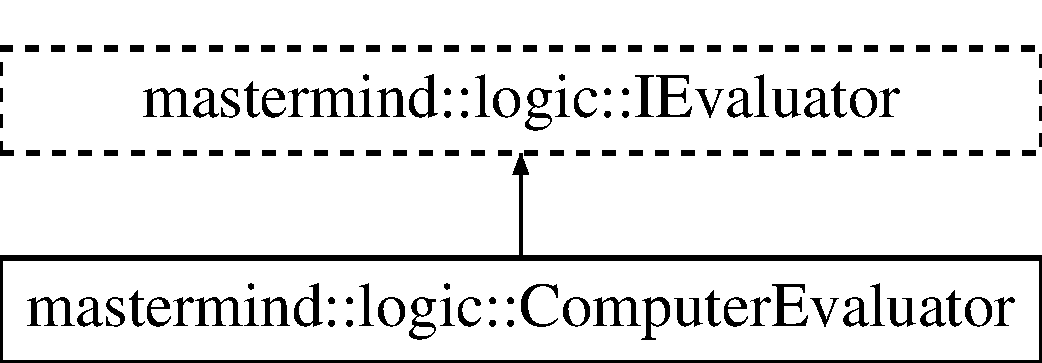
\includegraphics[height=2.000000cm]{classmastermind_1_1logic_1_1_computer_evaluator}
\end{center}
\end{figure}
\subsection*{Public Member Functions}
\begin{DoxyCompactItemize}
\item 
\hyperlink{classmastermind_1_1logic_1_1_computer_evaluator_a63c369068472dc8117552f991bd37a7a}{Computer\+Evaluator} (\hyperlink{classmastermind_1_1logic_1_1_color_code}{Color\+Code} solution\+Code)
\begin{DoxyCompactList}\small\item\em Create a \hyperlink{classmastermind_1_1logic_1_1_computer_evaluator}{Computer\+Evaluator}. \end{DoxyCompactList}\item 
\hyperlink{classmastermind_1_1logic_1_1_computer_evaluator_aa216efb1cb2e885562d01b76751c84be}{$\sim$\+Computer\+Evaluator} ()
\begin{DoxyCompactList}\small\item\em Destruct this. \end{DoxyCompactList}\item 
\hyperlink{classmastermind_1_1logic_1_1_black_and_white}{Black\+And\+White} $\ast$ \hyperlink{classmastermind_1_1logic_1_1_computer_evaluator_a579f808c46ab11077c4a3ce51838714b}{evaluate} (const \hyperlink{classmastermind_1_1logic_1_1_color_code}{Color\+Code} \&cc) override
\item 
\hyperlink{classmastermind_1_1logic_1_1_color_code}{Color\+Code} $\ast$ \hyperlink{classmastermind_1_1logic_1_1_computer_evaluator_ac6e0423a5ef2f6679cfe6be75d3a09dd}{get\+Solution} () override
\end{DoxyCompactItemize}
\subsection*{Additional Inherited Members}


\subsection{Detailed Description}
Evaluator which automatically evaluates the \hyperlink{classmastermind_1_1logic_1_1_color_code}{Color\+Code} given to a solution. 

\subsection{Constructor \& Destructor Documentation}
\hypertarget{classmastermind_1_1logic_1_1_computer_evaluator_a63c369068472dc8117552f991bd37a7a}{}\label{classmastermind_1_1logic_1_1_computer_evaluator_a63c369068472dc8117552f991bd37a7a} 
\index{mastermind\+::logic\+::\+Computer\+Evaluator@{mastermind\+::logic\+::\+Computer\+Evaluator}!Computer\+Evaluator@{Computer\+Evaluator}}
\index{Computer\+Evaluator@{Computer\+Evaluator}!mastermind\+::logic\+::\+Computer\+Evaluator@{mastermind\+::logic\+::\+Computer\+Evaluator}}
\subsubsection{\texorpdfstring{Computer\+Evaluator()}{ComputerEvaluator()}}
{\footnotesize\ttfamily mastermind\+::logic\+::\+Computer\+Evaluator\+::\+Computer\+Evaluator (\begin{DoxyParamCaption}\item[{\hyperlink{classmastermind_1_1logic_1_1_color_code}{Color\+Code}}]{solution\+Code }\end{DoxyParamCaption})}



Create a \hyperlink{classmastermind_1_1logic_1_1_computer_evaluator}{Computer\+Evaluator}. 


\begin{DoxyParams}{Parameters}
{\em solution\+Code} & the solution \\
\hline
\end{DoxyParams}
\hypertarget{classmastermind_1_1logic_1_1_computer_evaluator_aa216efb1cb2e885562d01b76751c84be}{}\label{classmastermind_1_1logic_1_1_computer_evaluator_aa216efb1cb2e885562d01b76751c84be} 
\index{mastermind\+::logic\+::\+Computer\+Evaluator@{mastermind\+::logic\+::\+Computer\+Evaluator}!````~Computer\+Evaluator@{$\sim$\+Computer\+Evaluator}}
\index{````~Computer\+Evaluator@{$\sim$\+Computer\+Evaluator}!mastermind\+::logic\+::\+Computer\+Evaluator@{mastermind\+::logic\+::\+Computer\+Evaluator}}
\subsubsection{\texorpdfstring{$\sim$\+Computer\+Evaluator()}{~ComputerEvaluator()}}
{\footnotesize\ttfamily mastermind\+::logic\+::\+Computer\+Evaluator\+::$\sim$\+Computer\+Evaluator (\begin{DoxyParamCaption}{ }\end{DoxyParamCaption})}



Destruct this. 



\subsection{Member Function Documentation}
\hypertarget{classmastermind_1_1logic_1_1_computer_evaluator_a579f808c46ab11077c4a3ce51838714b}{}\label{classmastermind_1_1logic_1_1_computer_evaluator_a579f808c46ab11077c4a3ce51838714b} 
\index{mastermind\+::logic\+::\+Computer\+Evaluator@{mastermind\+::logic\+::\+Computer\+Evaluator}!evaluate@{evaluate}}
\index{evaluate@{evaluate}!mastermind\+::logic\+::\+Computer\+Evaluator@{mastermind\+::logic\+::\+Computer\+Evaluator}}
\subsubsection{\texorpdfstring{evaluate()}{evaluate()}}
{\footnotesize\ttfamily \hyperlink{classmastermind_1_1logic_1_1_black_and_white}{Black\+And\+White} $\ast$ mastermind\+::logic\+::\+Computer\+Evaluator\+::evaluate (\begin{DoxyParamCaption}\item[{const \hyperlink{classmastermind_1_1logic_1_1_color_code}{Color\+Code} \&}]{cc }\end{DoxyParamCaption})\hspace{0.3cm}{\ttfamily [override]}}





\hypertarget{classmastermind_1_1logic_1_1_computer_evaluator_ac6e0423a5ef2f6679cfe6be75d3a09dd}{}\label{classmastermind_1_1logic_1_1_computer_evaluator_ac6e0423a5ef2f6679cfe6be75d3a09dd} 
\index{mastermind\+::logic\+::\+Computer\+Evaluator@{mastermind\+::logic\+::\+Computer\+Evaluator}!get\+Solution@{get\+Solution}}
\index{get\+Solution@{get\+Solution}!mastermind\+::logic\+::\+Computer\+Evaluator@{mastermind\+::logic\+::\+Computer\+Evaluator}}
\subsubsection{\texorpdfstring{get\+Solution()}{getSolution()}}
{\footnotesize\ttfamily \hyperlink{classmastermind_1_1logic_1_1_color_code}{Color\+Code} $\ast$ mastermind\+::logic\+::\+Computer\+Evaluator\+::get\+Solution (\begin{DoxyParamCaption}{ }\end{DoxyParamCaption})\hspace{0.3cm}{\ttfamily [override]}}







The documentation for this class was generated from the following files\+:\begin{DoxyCompactItemize}
\item 
Mastermind\+C\+P\+P\+D\+L\+L/\hyperlink{_computer_evaluator_8h}{Computer\+Evaluator.\+h}\item 
Mastermind\+C\+P\+P\+D\+L\+L/\hyperlink{_computer_evaluator_8cpp}{Computer\+Evaluator.\+cpp}\end{DoxyCompactItemize}

\hypertarget{classmastermind_1_1logic_1_1_computer_guesser}{}\section{mastermind\+:\+:logic\+:\+:Computer\+Guesser Class Reference}
\label{classmastermind_1_1logic_1_1_computer_guesser}\index{mastermind\+::logic\+::\+Computer\+Guesser@{mastermind\+::logic\+::\+Computer\+Guesser}}


A computer guesser. Uses a heuristic to find a solution. All possibilities are calculated and after each evaluation impossible solutions will be removed.  




{\ttfamily \#include $<$Computer\+Guesser.\+h$>$}

Inheritance diagram for mastermind\+:\+:logic\+:\+:Computer\+Guesser\+:\begin{figure}[H]
\begin{center}
\leavevmode
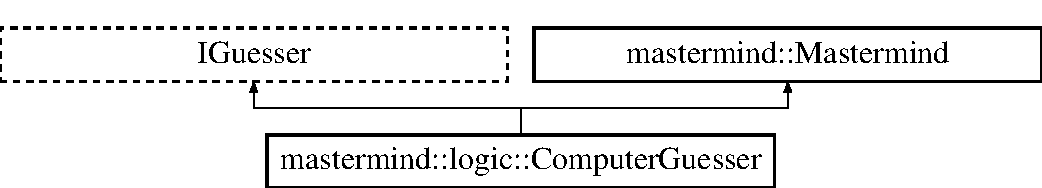
\includegraphics[height=2.000000cm]{classmastermind_1_1logic_1_1_computer_guesser}
\end{center}
\end{figure}
\subsection*{Public Member Functions}
\begin{DoxyCompactItemize}
\item 
\hyperlink{classmastermind_1_1logic_1_1_computer_guesser_a56134030aac585a8cdbe1e42d544b653}{Computer\+Guesser} ()
\begin{DoxyCompactList}\small\item\em Create a \hyperlink{classmastermind_1_1logic_1_1_computer_guesser}{Computer\+Guesser}. \end{DoxyCompactList}\item 
\hyperlink{classmastermind_1_1logic_1_1_color_code}{Color\+Code} $\ast$ \hyperlink{classmastermind_1_1logic_1_1_computer_guesser_a5553cb2d63534927fbf9031c5d40c828}{next\+Guess} () override
\item 
void \hyperlink{classmastermind_1_1logic_1_1_computer_guesser_a728f55a5700d3574fc6b9207c9e8db7d}{process\+Evaluation} (const \hyperlink{classmastermind_1_1logic_1_1_black_and_white}{Black\+And\+White} \&bw) override
\item 
bool \hyperlink{classmastermind_1_1logic_1_1_computer_guesser_ae93df46297030bcbd924f5ddc4af4889}{cheating\+Detected} () const
\begin{DoxyCompactList}\small\item\em Check if cheating was detected. \end{DoxyCompactList}\end{DoxyCompactItemize}
\subsection*{Additional Inherited Members}


\subsection{Detailed Description}
A computer guesser. Uses a heuristic to find a solution. All possibilities are calculated and after each evaluation impossible solutions will be removed. 

\subsection{Constructor \& Destructor Documentation}
\hypertarget{classmastermind_1_1logic_1_1_computer_guesser_a56134030aac585a8cdbe1e42d544b653}{}\label{classmastermind_1_1logic_1_1_computer_guesser_a56134030aac585a8cdbe1e42d544b653} 
\index{mastermind\+::logic\+::\+Computer\+Guesser@{mastermind\+::logic\+::\+Computer\+Guesser}!Computer\+Guesser@{Computer\+Guesser}}
\index{Computer\+Guesser@{Computer\+Guesser}!mastermind\+::logic\+::\+Computer\+Guesser@{mastermind\+::logic\+::\+Computer\+Guesser}}
\subsubsection{\texorpdfstring{Computer\+Guesser()}{ComputerGuesser()}}
{\footnotesize\ttfamily mastermind\+::logic\+::\+Computer\+Guesser\+::\+Computer\+Guesser (\begin{DoxyParamCaption}{ }\end{DoxyParamCaption})}



Create a \hyperlink{classmastermind_1_1logic_1_1_computer_guesser}{Computer\+Guesser}. 



\subsection{Member Function Documentation}
\hypertarget{classmastermind_1_1logic_1_1_computer_guesser_ae93df46297030bcbd924f5ddc4af4889}{}\label{classmastermind_1_1logic_1_1_computer_guesser_ae93df46297030bcbd924f5ddc4af4889} 
\index{mastermind\+::logic\+::\+Computer\+Guesser@{mastermind\+::logic\+::\+Computer\+Guesser}!cheating\+Detected@{cheating\+Detected}}
\index{cheating\+Detected@{cheating\+Detected}!mastermind\+::logic\+::\+Computer\+Guesser@{mastermind\+::logic\+::\+Computer\+Guesser}}
\subsubsection{\texorpdfstring{cheating\+Detected()}{cheatingDetected()}}
{\footnotesize\ttfamily bool mastermind\+::logic\+::\+Computer\+Guesser\+::cheating\+Detected (\begin{DoxyParamCaption}{ }\end{DoxyParamCaption}) const}



Check if cheating was detected. 

\begin{DoxyReturn}{Returns}
{\ttfamily true} if evaluator cheated 
\end{DoxyReturn}
\hypertarget{classmastermind_1_1logic_1_1_computer_guesser_a5553cb2d63534927fbf9031c5d40c828}{}\label{classmastermind_1_1logic_1_1_computer_guesser_a5553cb2d63534927fbf9031c5d40c828} 
\index{mastermind\+::logic\+::\+Computer\+Guesser@{mastermind\+::logic\+::\+Computer\+Guesser}!next\+Guess@{next\+Guess}}
\index{next\+Guess@{next\+Guess}!mastermind\+::logic\+::\+Computer\+Guesser@{mastermind\+::logic\+::\+Computer\+Guesser}}
\subsubsection{\texorpdfstring{next\+Guess()}{nextGuess()}}
{\footnotesize\ttfamily \hyperlink{classmastermind_1_1logic_1_1_color_code}{Color\+Code} $\ast$ mastermind\+::logic\+::\+Computer\+Guesser\+::next\+Guess (\begin{DoxyParamCaption}{ }\end{DoxyParamCaption})\hspace{0.3cm}{\ttfamily [override]}}





\hypertarget{classmastermind_1_1logic_1_1_computer_guesser_a728f55a5700d3574fc6b9207c9e8db7d}{}\label{classmastermind_1_1logic_1_1_computer_guesser_a728f55a5700d3574fc6b9207c9e8db7d} 
\index{mastermind\+::logic\+::\+Computer\+Guesser@{mastermind\+::logic\+::\+Computer\+Guesser}!process\+Evaluation@{process\+Evaluation}}
\index{process\+Evaluation@{process\+Evaluation}!mastermind\+::logic\+::\+Computer\+Guesser@{mastermind\+::logic\+::\+Computer\+Guesser}}
\subsubsection{\texorpdfstring{process\+Evaluation()}{processEvaluation()}}
{\footnotesize\ttfamily void mastermind\+::logic\+::\+Computer\+Guesser\+::process\+Evaluation (\begin{DoxyParamCaption}\item[{const \hyperlink{classmastermind_1_1logic_1_1_black_and_white}{Black\+And\+White} \&}]{bw }\end{DoxyParamCaption})\hspace{0.3cm}{\ttfamily [override]}}







The documentation for this class was generated from the following files\+:\begin{DoxyCompactItemize}
\item 
Mastermind\+C\+P\+P\+D\+L\+L/\hyperlink{_computer_guesser_8h}{Computer\+Guesser.\+h}\item 
Mastermind\+C\+P\+P\+D\+L\+L/\hyperlink{_computer_guesser_8cpp}{Computer\+Guesser.\+cpp}\end{DoxyCompactItemize}

\hypertarget{classmastermind_1_1logic_1_1_game_history}{}\section{mastermind\+:\+:logic\+:\+:Game\+History Class Reference}
\label{classmastermind_1_1logic_1_1_game_history}\index{mastermind\+::logic\+::\+Game\+History@{mastermind\+::logic\+::\+Game\+History}}


Game History. Saves performed moves, i.\+e. Color\+Codes and Black\+And\+Whites, so the board can be printed.  




{\ttfamily \#include $<$Game\+History.\+h$>$}

Inheritance diagram for mastermind\+:\+:logic\+:\+:Game\+History\+:\begin{figure}[H]
\begin{center}
\leavevmode
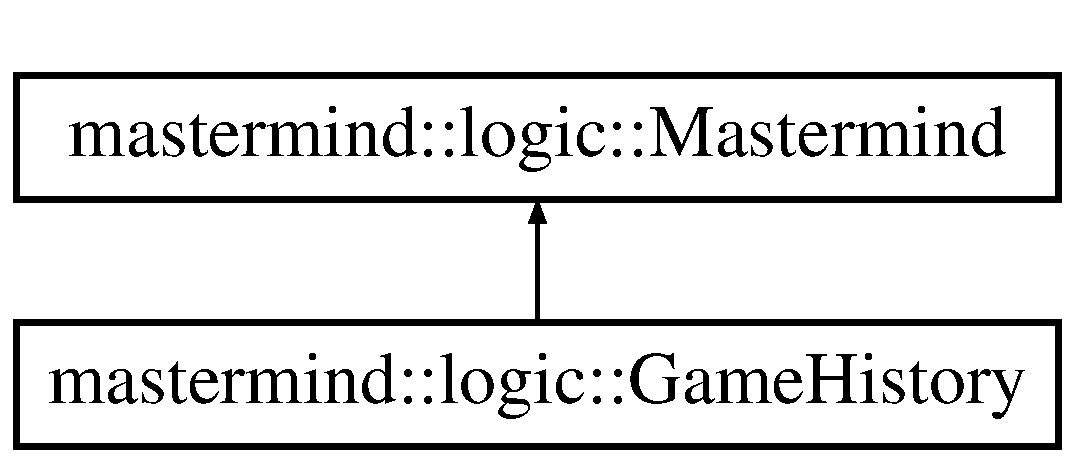
\includegraphics[height=2.000000cm]{classmastermind_1_1logic_1_1_game_history}
\end{center}
\end{figure}
\subsection*{Public Member Functions}
\begin{DoxyCompactItemize}
\item 
\hyperlink{classmastermind_1_1logic_1_1_game_history_a4731c4c94790c94c5f5e72a5ef344602}{Game\+History} ()
\begin{DoxyCompactList}\small\item\em Create empty history. \end{DoxyCompactList}\item 
\hyperlink{classmastermind_1_1logic_1_1_game_history_a7f94763f41492e795201f000874ba9e1}{$\sim$\+Game\+History} ()
\begin{DoxyCompactList}\small\item\em Destruct this. \end{DoxyCompactList}\item 
void \hyperlink{classmastermind_1_1logic_1_1_game_history_abcf47c78a6e9be8faa4238f2bc45e5e7}{add} (const \hyperlink{classmastermind_1_1logic_1_1_color_code}{Color\+Code} \&cc) const
\begin{DoxyCompactList}\small\item\em Add a \hyperlink{classmastermind_1_1logic_1_1_color_code}{Color\+Code} to the history. \end{DoxyCompactList}\item 
void \hyperlink{classmastermind_1_1logic_1_1_game_history_a0d81e90269bca2588b857c1c8bf966b8}{add} (const \hyperlink{classmastermind_1_1logic_1_1_black_and_white}{Black\+And\+White} \&bw) const
\begin{DoxyCompactList}\small\item\em Add a \hyperlink{classmastermind_1_1logic_1_1_black_and_white}{Black\+And\+White} to the history. \end{DoxyCompactList}\item 
std\+::wstring \hyperlink{classmastermind_1_1logic_1_1_game_history_ae3795a9ab89a850bc3b1f36d3ba76756}{to\+String} () const
\begin{DoxyCompactList}\small\item\em Get the string representation of the game history. \end{DoxyCompactList}\end{DoxyCompactItemize}
\subsection*{Private Attributes}
\begin{DoxyCompactItemize}
\item 
std\+::list$<$ \hyperlink{classmastermind_1_1logic_1_1_color_code}{Color\+Code} $>$ $\ast$const \hyperlink{classmastermind_1_1logic_1_1_game_history_a988bbccc372956773078e0e32344c1a9}{color\+Codes}
\begin{DoxyCompactList}\small\item\em History of Color\+Codes. \end{DoxyCompactList}\item 
std\+::list$<$ \hyperlink{classmastermind_1_1logic_1_1_black_and_white}{Black\+And\+White} $>$ $\ast$const \hyperlink{classmastermind_1_1logic_1_1_game_history_a60245b7b841a34c318dadfb953b4f512}{black\+And\+Whites}
\begin{DoxyCompactList}\small\item\em History of Black\+And\+Whites. \end{DoxyCompactList}\end{DoxyCompactItemize}
\subsection*{Additional Inherited Members}


\subsection{Detailed Description}
Game History. Saves performed moves, i.\+e. Color\+Codes and Black\+And\+Whites, so the board can be printed. 

\subsection{Constructor \& Destructor Documentation}
\hypertarget{classmastermind_1_1logic_1_1_game_history_a4731c4c94790c94c5f5e72a5ef344602}{}\label{classmastermind_1_1logic_1_1_game_history_a4731c4c94790c94c5f5e72a5ef344602} 
\index{mastermind\+::logic\+::\+Game\+History@{mastermind\+::logic\+::\+Game\+History}!Game\+History@{Game\+History}}
\index{Game\+History@{Game\+History}!mastermind\+::logic\+::\+Game\+History@{mastermind\+::logic\+::\+Game\+History}}
\subsubsection{\texorpdfstring{Game\+History()}{GameHistory()}}
{\footnotesize\ttfamily mastermind\+::logic\+::\+Game\+History\+::\+Game\+History (\begin{DoxyParamCaption}{ }\end{DoxyParamCaption})}



Create empty history. 

\hypertarget{classmastermind_1_1logic_1_1_game_history_a7f94763f41492e795201f000874ba9e1}{}\label{classmastermind_1_1logic_1_1_game_history_a7f94763f41492e795201f000874ba9e1} 
\index{mastermind\+::logic\+::\+Game\+History@{mastermind\+::logic\+::\+Game\+History}!````~Game\+History@{$\sim$\+Game\+History}}
\index{````~Game\+History@{$\sim$\+Game\+History}!mastermind\+::logic\+::\+Game\+History@{mastermind\+::logic\+::\+Game\+History}}
\subsubsection{\texorpdfstring{$\sim$\+Game\+History()}{~GameHistory()}}
{\footnotesize\ttfamily mastermind\+::logic\+::\+Game\+History\+::$\sim$\+Game\+History (\begin{DoxyParamCaption}{ }\end{DoxyParamCaption})}



Destruct this. 



\subsection{Member Function Documentation}
\hypertarget{classmastermind_1_1logic_1_1_game_history_abcf47c78a6e9be8faa4238f2bc45e5e7}{}\label{classmastermind_1_1logic_1_1_game_history_abcf47c78a6e9be8faa4238f2bc45e5e7} 
\index{mastermind\+::logic\+::\+Game\+History@{mastermind\+::logic\+::\+Game\+History}!add@{add}}
\index{add@{add}!mastermind\+::logic\+::\+Game\+History@{mastermind\+::logic\+::\+Game\+History}}
\subsubsection{\texorpdfstring{add()}{add()}\hspace{0.1cm}{\footnotesize\ttfamily [1/2]}}
{\footnotesize\ttfamily void mastermind\+::logic\+::\+Game\+History\+::add (\begin{DoxyParamCaption}\item[{const \hyperlink{classmastermind_1_1logic_1_1_color_code}{Color\+Code} \&}]{cc }\end{DoxyParamCaption}) const}



Add a \hyperlink{classmastermind_1_1logic_1_1_color_code}{Color\+Code} to the history. 


\begin{DoxyParams}{Parameters}
{\em cc} & the \hyperlink{classmastermind_1_1logic_1_1_color_code}{Color\+Code} \\
\hline
\end{DoxyParams}
\hypertarget{classmastermind_1_1logic_1_1_game_history_a0d81e90269bca2588b857c1c8bf966b8}{}\label{classmastermind_1_1logic_1_1_game_history_a0d81e90269bca2588b857c1c8bf966b8} 
\index{mastermind\+::logic\+::\+Game\+History@{mastermind\+::logic\+::\+Game\+History}!add@{add}}
\index{add@{add}!mastermind\+::logic\+::\+Game\+History@{mastermind\+::logic\+::\+Game\+History}}
\subsubsection{\texorpdfstring{add()}{add()}\hspace{0.1cm}{\footnotesize\ttfamily [2/2]}}
{\footnotesize\ttfamily void mastermind\+::logic\+::\+Game\+History\+::add (\begin{DoxyParamCaption}\item[{const \hyperlink{classmastermind_1_1logic_1_1_black_and_white}{Black\+And\+White} \&}]{bw }\end{DoxyParamCaption}) const}



Add a \hyperlink{classmastermind_1_1logic_1_1_black_and_white}{Black\+And\+White} to the history. 


\begin{DoxyParams}{Parameters}
{\em bw} & the \hyperlink{classmastermind_1_1logic_1_1_black_and_white}{Black\+And\+White} \\
\hline
\end{DoxyParams}
\hypertarget{classmastermind_1_1logic_1_1_game_history_ae3795a9ab89a850bc3b1f36d3ba76756}{}\label{classmastermind_1_1logic_1_1_game_history_ae3795a9ab89a850bc3b1f36d3ba76756} 
\index{mastermind\+::logic\+::\+Game\+History@{mastermind\+::logic\+::\+Game\+History}!to\+String@{to\+String}}
\index{to\+String@{to\+String}!mastermind\+::logic\+::\+Game\+History@{mastermind\+::logic\+::\+Game\+History}}
\subsubsection{\texorpdfstring{to\+String()}{toString()}}
{\footnotesize\ttfamily std\+::wstring mastermind\+::logic\+::\+Game\+History\+::to\+String (\begin{DoxyParamCaption}{ }\end{DoxyParamCaption}) const}



Get the string representation of the game history. 

\begin{DoxyReturn}{Returns}
the string 
\end{DoxyReturn}


\subsection{Member Data Documentation}
\hypertarget{classmastermind_1_1logic_1_1_game_history_a60245b7b841a34c318dadfb953b4f512}{}\label{classmastermind_1_1logic_1_1_game_history_a60245b7b841a34c318dadfb953b4f512} 
\index{mastermind\+::logic\+::\+Game\+History@{mastermind\+::logic\+::\+Game\+History}!black\+And\+Whites@{black\+And\+Whites}}
\index{black\+And\+Whites@{black\+And\+Whites}!mastermind\+::logic\+::\+Game\+History@{mastermind\+::logic\+::\+Game\+History}}
\subsubsection{\texorpdfstring{black\+And\+Whites}{blackAndWhites}}
{\footnotesize\ttfamily std\+::list$<$\hyperlink{classmastermind_1_1logic_1_1_black_and_white}{Black\+And\+White}$>$$\ast$ const mastermind\+::logic\+::\+Game\+History\+::black\+And\+Whites\hspace{0.3cm}{\ttfamily [private]}}



History of Black\+And\+Whites. 

\hypertarget{classmastermind_1_1logic_1_1_game_history_a988bbccc372956773078e0e32344c1a9}{}\label{classmastermind_1_1logic_1_1_game_history_a988bbccc372956773078e0e32344c1a9} 
\index{mastermind\+::logic\+::\+Game\+History@{mastermind\+::logic\+::\+Game\+History}!color\+Codes@{color\+Codes}}
\index{color\+Codes@{color\+Codes}!mastermind\+::logic\+::\+Game\+History@{mastermind\+::logic\+::\+Game\+History}}
\subsubsection{\texorpdfstring{color\+Codes}{colorCodes}}
{\footnotesize\ttfamily std\+::list$<$\hyperlink{classmastermind_1_1logic_1_1_color_code}{Color\+Code}$>$$\ast$ const mastermind\+::logic\+::\+Game\+History\+::color\+Codes\hspace{0.3cm}{\ttfamily [private]}}



History of Color\+Codes. 



The documentation for this class was generated from the following files\+:\begin{DoxyCompactItemize}
\item 
Mastermind\+C\+P\+P\+D\+L\+L/\hyperlink{_game_history_8h}{Game\+History.\+h}\item 
Mastermind\+C\+P\+P\+D\+L\+L/\hyperlink{_game_history_8cpp}{Game\+History.\+cpp}\end{DoxyCompactItemize}

\hypertarget{classmastermind_1_1logic_1_1_human_evaluator}{}\section{mastermind\+:\+:logic\+:\+:Human\+Evaluator Class Reference}
\label{classmastermind_1_1logic_1_1_human_evaluator}\index{mastermind\+::logic\+::\+Human\+Evaluator@{mastermind\+::logic\+::\+Human\+Evaluator}}


A human Evaluator for console.  




{\ttfamily \#include $<$Human\+Evaluator.\+h$>$}

Inheritance diagram for mastermind\+:\+:logic\+:\+:Human\+Evaluator\+:\begin{figure}[H]
\begin{center}
\leavevmode
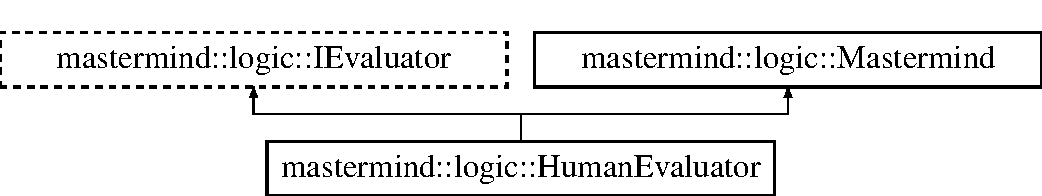
\includegraphics[height=2.000000cm]{classmastermind_1_1logic_1_1_human_evaluator}
\end{center}
\end{figure}
\subsection*{Public Member Functions}
\begin{DoxyCompactItemize}
\item 
\hyperlink{classmastermind_1_1logic_1_1_human_evaluator_ab1e96e3389a2932631a302e3cbaef8ff}{Human\+Evaluator} (\hyperlink{classmastermind_1_1logic_1_1_read_only_history}{Read\+Only\+History} $\ast$h)
\begin{DoxyCompactList}\small\item\em Create a \hyperlink{classmastermind_1_1logic_1_1_human_evaluator}{Human\+Evaluator}. \end{DoxyCompactList}\item 
\hyperlink{classmastermind_1_1logic_1_1_black_and_white}{Black\+And\+White} $\ast$ \hyperlink{classmastermind_1_1logic_1_1_human_evaluator_ac427121219b8e69ed30b0e123ce622a4}{evaluate} (const \hyperlink{classmastermind_1_1logic_1_1_color_code}{Color\+Code} \&cc) override
\item 
\hyperlink{classmastermind_1_1logic_1_1_color_code}{Color\+Code} $\ast$ \hyperlink{classmastermind_1_1logic_1_1_human_evaluator_ab369895151e4702e8b57d74c8f6869db}{get\+Solution} () override
\end{DoxyCompactItemize}
\subsection*{Additional Inherited Members}


\subsection{Detailed Description}
A human Evaluator for console. 

\subsection{Constructor \& Destructor Documentation}
\hypertarget{classmastermind_1_1logic_1_1_human_evaluator_ab1e96e3389a2932631a302e3cbaef8ff}{}\label{classmastermind_1_1logic_1_1_human_evaluator_ab1e96e3389a2932631a302e3cbaef8ff} 
\index{mastermind\+::logic\+::\+Human\+Evaluator@{mastermind\+::logic\+::\+Human\+Evaluator}!Human\+Evaluator@{Human\+Evaluator}}
\index{Human\+Evaluator@{Human\+Evaluator}!mastermind\+::logic\+::\+Human\+Evaluator@{mastermind\+::logic\+::\+Human\+Evaluator}}
\subsubsection{\texorpdfstring{Human\+Evaluator()}{HumanEvaluator()}}
{\footnotesize\ttfamily mastermind\+::logic\+::\+Human\+Evaluator\+::\+Human\+Evaluator (\begin{DoxyParamCaption}\item[{\hyperlink{classmastermind_1_1logic_1_1_read_only_history}{Read\+Only\+History} $\ast$}]{h }\end{DoxyParamCaption})}



Create a \hyperlink{classmastermind_1_1logic_1_1_human_evaluator}{Human\+Evaluator}. 


\begin{DoxyParams}{Parameters}
{\em h} & the history to read from \\
\hline
\end{DoxyParams}


\subsection{Member Function Documentation}
\hypertarget{classmastermind_1_1logic_1_1_human_evaluator_ac427121219b8e69ed30b0e123ce622a4}{}\label{classmastermind_1_1logic_1_1_human_evaluator_ac427121219b8e69ed30b0e123ce622a4} 
\index{mastermind\+::logic\+::\+Human\+Evaluator@{mastermind\+::logic\+::\+Human\+Evaluator}!evaluate@{evaluate}}
\index{evaluate@{evaluate}!mastermind\+::logic\+::\+Human\+Evaluator@{mastermind\+::logic\+::\+Human\+Evaluator}}
\subsubsection{\texorpdfstring{evaluate()}{evaluate()}}
{\footnotesize\ttfamily \hyperlink{classmastermind_1_1logic_1_1_black_and_white}{Black\+And\+White} $\ast$ mastermind\+::logic\+::\+Human\+Evaluator\+::evaluate (\begin{DoxyParamCaption}\item[{const \hyperlink{classmastermind_1_1logic_1_1_color_code}{Color\+Code} \&}]{cc }\end{DoxyParamCaption})\hspace{0.3cm}{\ttfamily [override]}}





\hypertarget{classmastermind_1_1logic_1_1_human_evaluator_ab369895151e4702e8b57d74c8f6869db}{}\label{classmastermind_1_1logic_1_1_human_evaluator_ab369895151e4702e8b57d74c8f6869db} 
\index{mastermind\+::logic\+::\+Human\+Evaluator@{mastermind\+::logic\+::\+Human\+Evaluator}!get\+Solution@{get\+Solution}}
\index{get\+Solution@{get\+Solution}!mastermind\+::logic\+::\+Human\+Evaluator@{mastermind\+::logic\+::\+Human\+Evaluator}}
\subsubsection{\texorpdfstring{get\+Solution()}{getSolution()}}
{\footnotesize\ttfamily \hyperlink{classmastermind_1_1logic_1_1_color_code}{Color\+Code} $\ast$ mastermind\+::logic\+::\+Human\+Evaluator\+::get\+Solution (\begin{DoxyParamCaption}{ }\end{DoxyParamCaption})\hspace{0.3cm}{\ttfamily [override]}}







The documentation for this class was generated from the following files\+:\begin{DoxyCompactItemize}
\item 
Mastermind\+C\+P\+P\+D\+L\+L/\hyperlink{_human_evaluator_8h}{Human\+Evaluator.\+h}\item 
Mastermind\+C\+P\+P\+D\+L\+L/\hyperlink{_human_evaluator_8cpp}{Human\+Evaluator.\+cpp}\end{DoxyCompactItemize}

\hypertarget{classmastermind_1_1logic_1_1_human_guesser}{}\section{mastermind\+:\+:logic\+:\+:Human\+Guesser Class Reference}
\label{classmastermind_1_1logic_1_1_human_guesser}\index{mastermind\+::logic\+::\+Human\+Guesser@{mastermind\+::logic\+::\+Human\+Guesser}}


A human guesser for console.  




{\ttfamily \#include $<$Human\+Guesser.\+h$>$}

Inheritance diagram for mastermind\+:\+:logic\+:\+:Human\+Guesser\+:\begin{figure}[H]
\begin{center}
\leavevmode
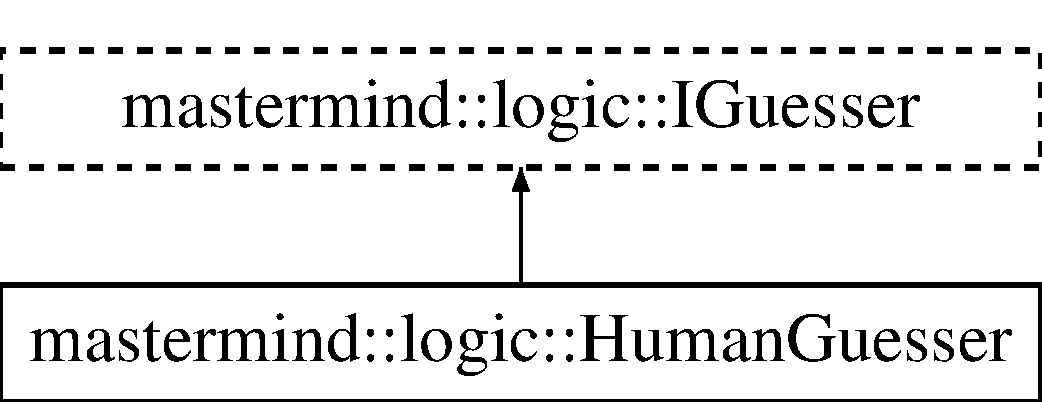
\includegraphics[height=2.000000cm]{classmastermind_1_1logic_1_1_human_guesser}
\end{center}
\end{figure}
\subsection*{Public Member Functions}
\begin{DoxyCompactItemize}
\item 
\hyperlink{classmastermind_1_1logic_1_1_human_guesser_a8898e930a7d0fd76d796844f600f34de}{Human\+Guesser} (const \hyperlink{classmastermind_1_1logic_1_1_mastermind}{Mastermind} $\ast$\hyperlink{classmastermind_1_1logic_1_1_human_guesser_a36934ed862366c1d0e15e14302a23ff8}{game}, \hyperlink{classmastermind_1_1logic_1_1_read_only_history}{Read\+Only\+History} $\ast$h)
\begin{DoxyCompactList}\small\item\em Create a \hyperlink{classmastermind_1_1logic_1_1_human_guesser}{Human\+Guesser}. \end{DoxyCompactList}\item 
\hyperlink{classmastermind_1_1logic_1_1_color_code}{Color\+Code} $\ast$ \hyperlink{classmastermind_1_1logic_1_1_human_guesser_a5a165250f667fd40099c43cd3caf487c}{next\+Guess} () override
\begin{DoxyCompactList}\small\item\em Get the next guess. \end{DoxyCompactList}\item 
void \hyperlink{classmastermind_1_1logic_1_1_human_guesser_ad1c868e2dac07c1af9bb8935783e2e9b}{process\+Evaluation} (const \hyperlink{classmastermind_1_1logic_1_1_black_and_white}{Black\+And\+White} \&bw) override
\begin{DoxyCompactList}\small\item\em Process evaluation. This method processes the other player\textquotesingle{}s feedback on the last guess provided by {\ttfamily next\+Guess}. Must only be executed if {\ttfamily next\+Guess} has been called before and has not returned {\ttfamily null}. \end{DoxyCompactList}\end{DoxyCompactItemize}
\subsection*{Private Attributes}
\begin{DoxyCompactItemize}
\item 
const \hyperlink{classmastermind_1_1logic_1_1_mastermind}{Mastermind} $\ast$ \hyperlink{classmastermind_1_1logic_1_1_human_guesser_a36934ed862366c1d0e15e14302a23ff8}{game}
\begin{DoxyCompactList}\small\item\em Base game. \end{DoxyCompactList}\item 
\hyperlink{classmastermind_1_1logic_1_1_read_only_history}{Read\+Only\+History} $\ast$const \hyperlink{classmastermind_1_1logic_1_1_human_guesser_aa6d916119121bed7fbdf7f1af9807b58}{history}
\begin{DoxyCompactList}\small\item\em History for the evaluator. Used for print. \end{DoxyCompactList}\item 
const std\+::wstring \hyperlink{classmastermind_1_1logic_1_1_human_guesser_a8df8372c5f59e73e88ad023dd66d590f}{H\+E\+L\+P\+\_\+\+T\+E\+XT}
\begin{DoxyCompactList}\small\item\em The help text for console output. \end{DoxyCompactList}\end{DoxyCompactItemize}


\subsection{Detailed Description}
A human guesser for console. 

\subsection{Constructor \& Destructor Documentation}
\hypertarget{classmastermind_1_1logic_1_1_human_guesser_a8898e930a7d0fd76d796844f600f34de}{}\label{classmastermind_1_1logic_1_1_human_guesser_a8898e930a7d0fd76d796844f600f34de} 
\index{mastermind\+::logic\+::\+Human\+Guesser@{mastermind\+::logic\+::\+Human\+Guesser}!Human\+Guesser@{Human\+Guesser}}
\index{Human\+Guesser@{Human\+Guesser}!mastermind\+::logic\+::\+Human\+Guesser@{mastermind\+::logic\+::\+Human\+Guesser}}
\subsubsection{\texorpdfstring{Human\+Guesser()}{HumanGuesser()}}
{\footnotesize\ttfamily mastermind\+::logic\+::\+Human\+Guesser\+::\+Human\+Guesser (\begin{DoxyParamCaption}\item[{const \hyperlink{classmastermind_1_1logic_1_1_mastermind}{Mastermind} $\ast$}]{game,  }\item[{\hyperlink{classmastermind_1_1logic_1_1_read_only_history}{Read\+Only\+History} $\ast$}]{h }\end{DoxyParamCaption})}



Create a \hyperlink{classmastermind_1_1logic_1_1_human_guesser}{Human\+Guesser}. 


\begin{DoxyParams}{Parameters}
{\em game} & the main game, must not be {\ttfamily nullptr} \\
\hline
{\em h} & the history to read from, must not be {\ttfamily nullptr} \\
\hline
\end{DoxyParams}


\subsection{Member Function Documentation}
\hypertarget{classmastermind_1_1logic_1_1_human_guesser_a5a165250f667fd40099c43cd3caf487c}{}\label{classmastermind_1_1logic_1_1_human_guesser_a5a165250f667fd40099c43cd3caf487c} 
\index{mastermind\+::logic\+::\+Human\+Guesser@{mastermind\+::logic\+::\+Human\+Guesser}!next\+Guess@{next\+Guess}}
\index{next\+Guess@{next\+Guess}!mastermind\+::logic\+::\+Human\+Guesser@{mastermind\+::logic\+::\+Human\+Guesser}}
\subsubsection{\texorpdfstring{next\+Guess()}{nextGuess()}}
{\footnotesize\ttfamily \hyperlink{classmastermind_1_1logic_1_1_color_code}{Color\+Code} $\ast$ mastermind\+::logic\+::\+Human\+Guesser\+::next\+Guess (\begin{DoxyParamCaption}{ }\end{DoxyParamCaption})\hspace{0.3cm}{\ttfamily [override]}, {\ttfamily [virtual]}}



Get the next guess. 

\begin{DoxyReturn}{Returns}
The next guess of the player. {\ttfamily null} aborts the game. 
\end{DoxyReturn}


Implements \hyperlink{classmastermind_1_1logic_1_1_i_guesser_a285f709f2076098acb5bc7c49a1435c7}{mastermind\+::logic\+::\+I\+Guesser}.

\hypertarget{classmastermind_1_1logic_1_1_human_guesser_ad1c868e2dac07c1af9bb8935783e2e9b}{}\label{classmastermind_1_1logic_1_1_human_guesser_ad1c868e2dac07c1af9bb8935783e2e9b} 
\index{mastermind\+::logic\+::\+Human\+Guesser@{mastermind\+::logic\+::\+Human\+Guesser}!process\+Evaluation@{process\+Evaluation}}
\index{process\+Evaluation@{process\+Evaluation}!mastermind\+::logic\+::\+Human\+Guesser@{mastermind\+::logic\+::\+Human\+Guesser}}
\subsubsection{\texorpdfstring{process\+Evaluation()}{processEvaluation()}}
{\footnotesize\ttfamily void mastermind\+::logic\+::\+Human\+Guesser\+::process\+Evaluation (\begin{DoxyParamCaption}\item[{const \hyperlink{classmastermind_1_1logic_1_1_black_and_white}{Black\+And\+White} \&}]{bw }\end{DoxyParamCaption})\hspace{0.3cm}{\ttfamily [override]}, {\ttfamily [virtual]}}



Process evaluation. This method processes the other player\textquotesingle{}s feedback on the last guess provided by {\ttfamily next\+Guess}. Must only be executed if {\ttfamily next\+Guess} has been called before and has not returned {\ttfamily null}. 


\begin{DoxyParams}{Parameters}
{\em bw} & Evaluation of the last guess. \\
\hline
\end{DoxyParams}


Implements \hyperlink{classmastermind_1_1logic_1_1_i_guesser_a83a8fbd8aed3c4fa8c7a023fd7ebd6e7}{mastermind\+::logic\+::\+I\+Guesser}.



\subsection{Member Data Documentation}
\hypertarget{classmastermind_1_1logic_1_1_human_guesser_a36934ed862366c1d0e15e14302a23ff8}{}\label{classmastermind_1_1logic_1_1_human_guesser_a36934ed862366c1d0e15e14302a23ff8} 
\index{mastermind\+::logic\+::\+Human\+Guesser@{mastermind\+::logic\+::\+Human\+Guesser}!game@{game}}
\index{game@{game}!mastermind\+::logic\+::\+Human\+Guesser@{mastermind\+::logic\+::\+Human\+Guesser}}
\subsubsection{\texorpdfstring{game}{game}}
{\footnotesize\ttfamily const \hyperlink{classmastermind_1_1logic_1_1_mastermind}{Mastermind}$\ast$ mastermind\+::logic\+::\+Human\+Guesser\+::game\hspace{0.3cm}{\ttfamily [private]}}



Base game. 

\hypertarget{classmastermind_1_1logic_1_1_human_guesser_a8df8372c5f59e73e88ad023dd66d590f}{}\label{classmastermind_1_1logic_1_1_human_guesser_a8df8372c5f59e73e88ad023dd66d590f} 
\index{mastermind\+::logic\+::\+Human\+Guesser@{mastermind\+::logic\+::\+Human\+Guesser}!H\+E\+L\+P\+\_\+\+T\+E\+XT@{H\+E\+L\+P\+\_\+\+T\+E\+XT}}
\index{H\+E\+L\+P\+\_\+\+T\+E\+XT@{H\+E\+L\+P\+\_\+\+T\+E\+XT}!mastermind\+::logic\+::\+Human\+Guesser@{mastermind\+::logic\+::\+Human\+Guesser}}
\subsubsection{\texorpdfstring{H\+E\+L\+P\+\_\+\+T\+E\+XT}{HELP\_TEXT}}
{\footnotesize\ttfamily const std\+::wstring mastermind\+::logic\+::\+Human\+Guesser\+::\+H\+E\+L\+P\+\_\+\+T\+E\+XT\hspace{0.3cm}{\ttfamily [private]}}



The help text for console output. 

\hypertarget{classmastermind_1_1logic_1_1_human_guesser_aa6d916119121bed7fbdf7f1af9807b58}{}\label{classmastermind_1_1logic_1_1_human_guesser_aa6d916119121bed7fbdf7f1af9807b58} 
\index{mastermind\+::logic\+::\+Human\+Guesser@{mastermind\+::logic\+::\+Human\+Guesser}!history@{history}}
\index{history@{history}!mastermind\+::logic\+::\+Human\+Guesser@{mastermind\+::logic\+::\+Human\+Guesser}}
\subsubsection{\texorpdfstring{history}{history}}
{\footnotesize\ttfamily \hyperlink{classmastermind_1_1logic_1_1_read_only_history}{Read\+Only\+History}$\ast$ const mastermind\+::logic\+::\+Human\+Guesser\+::history\hspace{0.3cm}{\ttfamily [private]}}



History for the evaluator. Used for print. 



The documentation for this class was generated from the following files\+:\begin{DoxyCompactItemize}
\item 
Mastermind\+C\+P\+P\+D\+L\+L/\hyperlink{_human_guesser_8h}{Human\+Guesser.\+h}\item 
Mastermind\+C\+P\+P\+D\+L\+L/\hyperlink{_human_guesser_8cpp}{Human\+Guesser.\+cpp}\end{DoxyCompactItemize}

\hypertarget{classmastermind_1_1logic_1_1_i_evaluator}{}\section{mastermind\+:\+:logic\+:\+:I\+Evaluator Class Reference}
\label{classmastermind_1_1logic_1_1_i_evaluator}\index{mastermind\+::logic\+::\+I\+Evaluator@{mastermind\+::logic\+::\+I\+Evaluator}}


Interface for an Evaluator of a \hyperlink{classmastermind_1_1logic_1_1_color_code}{Color\+Code}. This interface class should be abstract however Doxygen has parsing problems then.  




{\ttfamily \#include $<$I\+Evaluator.\+h$>$}

Inheritance diagram for mastermind\+:\+:logic\+:\+:I\+Evaluator\+:\begin{figure}[H]
\begin{center}
\leavevmode
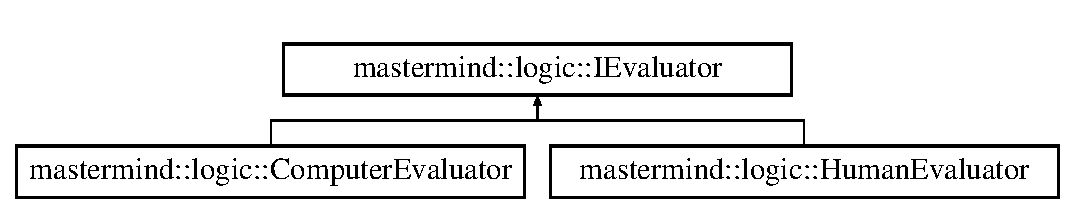
\includegraphics[height=2.000000cm]{classmastermind_1_1logic_1_1_i_evaluator}
\end{center}
\end{figure}
\subsection*{Public Member Functions}
\begin{DoxyCompactItemize}
\item 
virtual \hyperlink{classmastermind_1_1logic_1_1_i_evaluator_a77766402180f37bce062b808feb5cee6}{$\sim$\+I\+Evaluator} ()
\item 
virtual \hyperlink{classmastermind_1_1logic_1_1_black_and_white}{Black\+And\+White} $\ast$ \hyperlink{classmastermind_1_1logic_1_1_i_evaluator_a1ac9459cbb3698affa4154388b019f09}{evaluate} (const \hyperlink{classmastermind_1_1logic_1_1_color_code}{Color\+Code} $\ast$cc) override
\begin{DoxyCompactList}\small\item\em Evaluate the given \hyperlink{classmastermind_1_1logic_1_1_color_code}{Color\+Code} to the respective \hyperlink{classmastermind_1_1logic_1_1_black_and_white}{Black\+And\+White}. \end{DoxyCompactList}\item 
virtual \hyperlink{classmastermind_1_1logic_1_1_color_code}{Color\+Code} $\ast$ \hyperlink{classmastermind_1_1logic_1_1_i_evaluator_a544ecf5ba1d2cb5708e62fc508d341f3}{get\+Solution} () override
\begin{DoxyCompactList}\small\item\em Get the solution. \end{DoxyCompactList}\end{DoxyCompactItemize}


\subsection{Detailed Description}
Interface for an Evaluator of a \hyperlink{classmastermind_1_1logic_1_1_color_code}{Color\+Code}. This interface class should be abstract however Doxygen has parsing problems then. 

\subsection{Constructor \& Destructor Documentation}
\hypertarget{classmastermind_1_1logic_1_1_i_evaluator_a77766402180f37bce062b808feb5cee6}{}\label{classmastermind_1_1logic_1_1_i_evaluator_a77766402180f37bce062b808feb5cee6} 
\index{mastermind\+::logic\+::\+I\+Evaluator@{mastermind\+::logic\+::\+I\+Evaluator}!````~I\+Evaluator@{$\sim$\+I\+Evaluator}}
\index{````~I\+Evaluator@{$\sim$\+I\+Evaluator}!mastermind\+::logic\+::\+I\+Evaluator@{mastermind\+::logic\+::\+I\+Evaluator}}
\subsubsection{\texorpdfstring{$\sim$\+I\+Evaluator()}{~IEvaluator()}}
{\footnotesize\ttfamily virtual mastermind\+::logic\+::\+I\+Evaluator\+::$\sim$\+I\+Evaluator (\begin{DoxyParamCaption}{ }\end{DoxyParamCaption})\hspace{0.3cm}{\ttfamily [inline]}, {\ttfamily [virtual]}}



\subsection{Member Function Documentation}
\hypertarget{classmastermind_1_1logic_1_1_i_evaluator_a1ac9459cbb3698affa4154388b019f09}{}\label{classmastermind_1_1logic_1_1_i_evaluator_a1ac9459cbb3698affa4154388b019f09} 
\index{mastermind\+::logic\+::\+I\+Evaluator@{mastermind\+::logic\+::\+I\+Evaluator}!evaluate@{evaluate}}
\index{evaluate@{evaluate}!mastermind\+::logic\+::\+I\+Evaluator@{mastermind\+::logic\+::\+I\+Evaluator}}
\subsubsection{\texorpdfstring{evaluate()}{evaluate()}}
{\footnotesize\ttfamily virtual \hyperlink{classmastermind_1_1logic_1_1_black_and_white}{Black\+And\+White}$\ast$ mastermind\+::logic\+::\+I\+Evaluator\+::evaluate (\begin{DoxyParamCaption}\item[{const \hyperlink{classmastermind_1_1logic_1_1_color_code}{Color\+Code} $\ast$}]{cc }\end{DoxyParamCaption})\hspace{0.3cm}{\ttfamily [pure virtual]}}



Evaluate the given \hyperlink{classmastermind_1_1logic_1_1_color_code}{Color\+Code} to the respective \hyperlink{classmastermind_1_1logic_1_1_black_and_white}{Black\+And\+White}. 


\begin{DoxyParams}{Parameters}
{\em cc} & the \hyperlink{classmastermind_1_1logic_1_1_color_code}{Color\+Code} to be evaluated, must not be {\ttfamily null} \\
\hline
\end{DoxyParams}
\begin{DoxyReturn}{Returns}
the resulting \hyperlink{classmastermind_1_1logic_1_1_black_and_white}{Black\+And\+White} 
\end{DoxyReturn}


Implemented in \hyperlink{classmastermind_1_1logic_1_1_computer_evaluator_a65f4a9bafcd5240e0cf92f6398025bd5}{mastermind\+::logic\+::\+Computer\+Evaluator}, and \hyperlink{classmastermind_1_1logic_1_1_human_evaluator_a12080bafb5e428db8cf8b8173821f83d}{mastermind\+::logic\+::\+Human\+Evaluator}.

\hypertarget{classmastermind_1_1logic_1_1_i_evaluator_a544ecf5ba1d2cb5708e62fc508d341f3}{}\label{classmastermind_1_1logic_1_1_i_evaluator_a544ecf5ba1d2cb5708e62fc508d341f3} 
\index{mastermind\+::logic\+::\+I\+Evaluator@{mastermind\+::logic\+::\+I\+Evaluator}!get\+Solution@{get\+Solution}}
\index{get\+Solution@{get\+Solution}!mastermind\+::logic\+::\+I\+Evaluator@{mastermind\+::logic\+::\+I\+Evaluator}}
\subsubsection{\texorpdfstring{get\+Solution()}{getSolution()}}
{\footnotesize\ttfamily virtual \hyperlink{classmastermind_1_1logic_1_1_color_code}{Color\+Code}$\ast$ mastermind\+::logic\+::\+I\+Evaluator\+::get\+Solution (\begin{DoxyParamCaption}{ }\end{DoxyParamCaption})\hspace{0.3cm}{\ttfamily [pure virtual]}}



Get the solution. 

\begin{DoxyReturn}{Returns}
the solution \hyperlink{classmastermind_1_1logic_1_1_color_code}{Color\+Code} or N\+U\+LL if not available yet. 
\end{DoxyReturn}


Implemented in \hyperlink{classmastermind_1_1logic_1_1_computer_evaluator_ac6e0423a5ef2f6679cfe6be75d3a09dd}{mastermind\+::logic\+::\+Computer\+Evaluator}, and \hyperlink{classmastermind_1_1logic_1_1_human_evaluator_ab369895151e4702e8b57d74c8f6869db}{mastermind\+::logic\+::\+Human\+Evaluator}.



The documentation for this class was generated from the following file\+:\begin{DoxyCompactItemize}
\item 
Mastermind\+C\+P\+P\+D\+L\+L/\hyperlink{_i_evaluator_8h}{I\+Evaluator.\+h}\end{DoxyCompactItemize}

\hypertarget{classmastermind_1_1logic_1_1_i_guesser}{}\section{mastermind\+:\+:logic\+:\+:I\+Guesser Class Reference}
\label{classmastermind_1_1logic_1_1_i_guesser}\index{mastermind\+::logic\+::\+I\+Guesser@{mastermind\+::logic\+::\+I\+Guesser}}


Interface for a Guesser. This interface class should be abstract however Doxygen has parsing problems then.  




{\ttfamily \#include $<$I\+Guesser.\+h$>$}

Inheritance diagram for mastermind\+:\+:logic\+:\+:I\+Guesser\+:\begin{figure}[H]
\begin{center}
\leavevmode
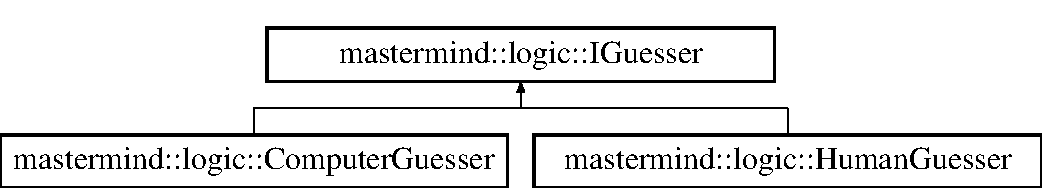
\includegraphics[height=2.000000cm]{classmastermind_1_1logic_1_1_i_guesser}
\end{center}
\end{figure}
\subsection*{Public Member Functions}
\begin{DoxyCompactItemize}
\item 
virtual \hyperlink{classmastermind_1_1logic_1_1_i_guesser_a43ad2f926001589dd454925b839ab106}{$\sim$\+I\+Guesser} ()
\item 
virtual \hyperlink{classmastermind_1_1logic_1_1_color_code}{Color\+Code} $\ast$ \hyperlink{classmastermind_1_1logic_1_1_i_guesser_a285f709f2076098acb5bc7c49a1435c7}{next\+Guess} () override
\begin{DoxyCompactList}\small\item\em Get the next guess. \end{DoxyCompactList}\item 
virtual void \hyperlink{classmastermind_1_1logic_1_1_i_guesser_a83a8fbd8aed3c4fa8c7a023fd7ebd6e7}{process\+Evaluation} (const \hyperlink{classmastermind_1_1logic_1_1_black_and_white}{Black\+And\+White} \&bw) override
\begin{DoxyCompactList}\small\item\em Process evaluation. This method processes the other player\textquotesingle{}s feedback on the last guess provided by {\ttfamily next\+Guess}. Must only be executed if {\ttfamily next\+Guess} has been called before and has not returned {\ttfamily null}. \end{DoxyCompactList}\end{DoxyCompactItemize}


\subsection{Detailed Description}
Interface for a Guesser. This interface class should be abstract however Doxygen has parsing problems then. 

\subsection{Constructor \& Destructor Documentation}
\hypertarget{classmastermind_1_1logic_1_1_i_guesser_a43ad2f926001589dd454925b839ab106}{}\label{classmastermind_1_1logic_1_1_i_guesser_a43ad2f926001589dd454925b839ab106} 
\index{mastermind\+::logic\+::\+I\+Guesser@{mastermind\+::logic\+::\+I\+Guesser}!````~I\+Guesser@{$\sim$\+I\+Guesser}}
\index{````~I\+Guesser@{$\sim$\+I\+Guesser}!mastermind\+::logic\+::\+I\+Guesser@{mastermind\+::logic\+::\+I\+Guesser}}
\subsubsection{\texorpdfstring{$\sim$\+I\+Guesser()}{~IGuesser()}}
{\footnotesize\ttfamily virtual mastermind\+::logic\+::\+I\+Guesser\+::$\sim$\+I\+Guesser (\begin{DoxyParamCaption}{ }\end{DoxyParamCaption})\hspace{0.3cm}{\ttfamily [inline]}, {\ttfamily [virtual]}}



\subsection{Member Function Documentation}
\hypertarget{classmastermind_1_1logic_1_1_i_guesser_a285f709f2076098acb5bc7c49a1435c7}{}\label{classmastermind_1_1logic_1_1_i_guesser_a285f709f2076098acb5bc7c49a1435c7} 
\index{mastermind\+::logic\+::\+I\+Guesser@{mastermind\+::logic\+::\+I\+Guesser}!next\+Guess@{next\+Guess}}
\index{next\+Guess@{next\+Guess}!mastermind\+::logic\+::\+I\+Guesser@{mastermind\+::logic\+::\+I\+Guesser}}
\subsubsection{\texorpdfstring{next\+Guess()}{nextGuess()}}
{\footnotesize\ttfamily virtual \hyperlink{classmastermind_1_1logic_1_1_color_code}{Color\+Code}$\ast$ mastermind\+::logic\+::\+I\+Guesser\+::next\+Guess (\begin{DoxyParamCaption}{ }\end{DoxyParamCaption})\hspace{0.3cm}{\ttfamily [pure virtual]}}



Get the next guess. 

\begin{DoxyReturn}{Returns}
The next guess of the player. {\ttfamily null} aborts the game. 
\end{DoxyReturn}


Implemented in \hyperlink{classmastermind_1_1logic_1_1_computer_guesser_a5553cb2d63534927fbf9031c5d40c828}{mastermind\+::logic\+::\+Computer\+Guesser}, and \hyperlink{classmastermind_1_1logic_1_1_human_guesser_a5a165250f667fd40099c43cd3caf487c}{mastermind\+::logic\+::\+Human\+Guesser}.

\hypertarget{classmastermind_1_1logic_1_1_i_guesser_a83a8fbd8aed3c4fa8c7a023fd7ebd6e7}{}\label{classmastermind_1_1logic_1_1_i_guesser_a83a8fbd8aed3c4fa8c7a023fd7ebd6e7} 
\index{mastermind\+::logic\+::\+I\+Guesser@{mastermind\+::logic\+::\+I\+Guesser}!process\+Evaluation@{process\+Evaluation}}
\index{process\+Evaluation@{process\+Evaluation}!mastermind\+::logic\+::\+I\+Guesser@{mastermind\+::logic\+::\+I\+Guesser}}
\subsubsection{\texorpdfstring{process\+Evaluation()}{processEvaluation()}}
{\footnotesize\ttfamily virtual void mastermind\+::logic\+::\+I\+Guesser\+::process\+Evaluation (\begin{DoxyParamCaption}\item[{const \hyperlink{classmastermind_1_1logic_1_1_black_and_white}{Black\+And\+White} \&}]{bw }\end{DoxyParamCaption})\hspace{0.3cm}{\ttfamily [pure virtual]}}



Process evaluation. This method processes the other player\textquotesingle{}s feedback on the last guess provided by {\ttfamily next\+Guess}. Must only be executed if {\ttfamily next\+Guess} has been called before and has not returned {\ttfamily null}. 


\begin{DoxyParams}{Parameters}
{\em bw} & Evaluation of the last guess. \\
\hline
\end{DoxyParams}


Implemented in \hyperlink{classmastermind_1_1logic_1_1_computer_guesser_a728f55a5700d3574fc6b9207c9e8db7d}{mastermind\+::logic\+::\+Computer\+Guesser}, and \hyperlink{classmastermind_1_1logic_1_1_human_guesser_ad1c868e2dac07c1af9bb8935783e2e9b}{mastermind\+::logic\+::\+Human\+Guesser}.



The documentation for this class was generated from the following file\+:\begin{DoxyCompactItemize}
\item 
Mastermind\+C\+P\+P\+D\+L\+L/\hyperlink{_i_guesser_8h}{I\+Guesser.\+h}\end{DoxyCompactItemize}

\hypertarget{classmastermind_1_1logic_1_1_main_game}{}\section{mastermind\+:\+:logic\+:\+:Main\+Game Class Reference}
\label{classmastermind_1_1logic_1_1_main_game}\index{mastermind\+::logic\+::\+Main\+Game@{mastermind\+::logic\+::\+Main\+Game}}


The Game. Game logic is in here. No in and output. Works only with the interfaces of I\+Evaluator and I\+Guesser.  




{\ttfamily \#include $<$Main\+Game.\+h$>$}

Inheritance diagram for mastermind\+:\+:logic\+:\+:Main\+Game\+:\begin{figure}[H]
\begin{center}
\leavevmode
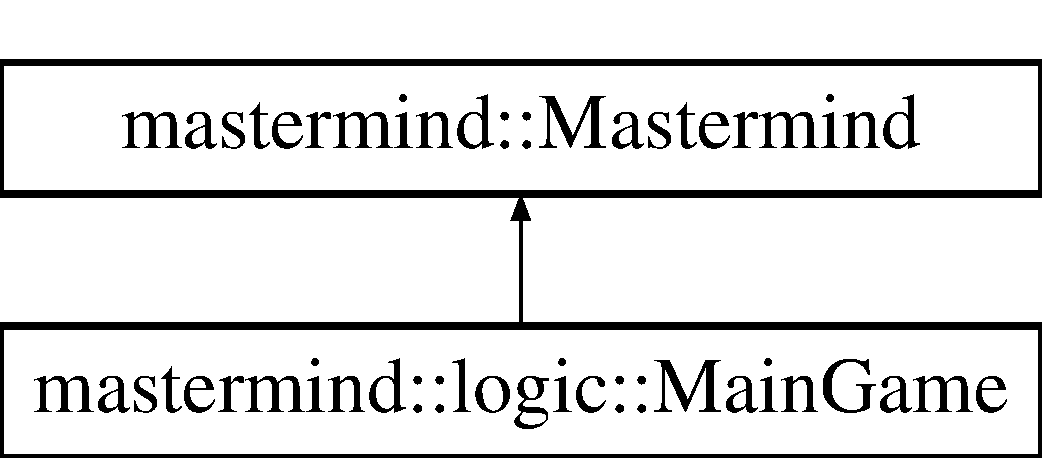
\includegraphics[height=2.000000cm]{classmastermind_1_1logic_1_1_main_game}
\end{center}
\end{figure}
\subsection*{Public Member Functions}
\begin{DoxyCompactItemize}
\item 
\hyperlink{classmastermind_1_1logic_1_1_main_game_af1a4d71009b1d4322edec911ea39b55c}{Main\+Game} (I\+Guesser $\ast$g, I\+Evaluator $\ast$e, \hyperlink{classmastermind_1_1logic_1_1_game_history}{Game\+History} $\ast$h)
\item 
bool \hyperlink{classmastermind_1_1logic_1_1_main_game_a2b48f18cf8dbd95431d4627b57ea5d01}{next} ()
\begin{DoxyCompactList}\small\item\em The game itself. Performs the next turn, i.\+e.\+one turn each of Guesser and Evaluator. \end{DoxyCompactList}\end{DoxyCompactItemize}
\subsection*{Additional Inherited Members}


\subsection{Detailed Description}
The Game. Game logic is in here. No in and output. Works only with the interfaces of I\+Evaluator and I\+Guesser. 

\subsection{Constructor \& Destructor Documentation}
\hypertarget{classmastermind_1_1logic_1_1_main_game_af1a4d71009b1d4322edec911ea39b55c}{}\label{classmastermind_1_1logic_1_1_main_game_af1a4d71009b1d4322edec911ea39b55c} 
\index{mastermind\+::logic\+::\+Main\+Game@{mastermind\+::logic\+::\+Main\+Game}!Main\+Game@{Main\+Game}}
\index{Main\+Game@{Main\+Game}!mastermind\+::logic\+::\+Main\+Game@{mastermind\+::logic\+::\+Main\+Game}}
\subsubsection{\texorpdfstring{Main\+Game()}{MainGame()}}
{\footnotesize\ttfamily mastermind\+::logic\+::\+Main\+Game\+::\+Main\+Game (\begin{DoxyParamCaption}\item[{I\+Guesser $\ast$}]{g,  }\item[{I\+Evaluator $\ast$}]{e,  }\item[{\hyperlink{classmastermind_1_1logic_1_1_game_history}{Game\+History} $\ast$}]{h }\end{DoxyParamCaption})}

Creates a \hyperlink{classmastermind_1_1logic_1_1_main_game}{Main\+Game} object. 
\begin{DoxyParams}{Parameters}
{\em g} & the guesser, must not be {\ttfamily null} \\
\hline
{\em e} & the evaluator, must not be {\ttfamily null} \\
\hline
{\em h} & the history to write to, must not be {\ttfamily null} \\
\hline
\end{DoxyParams}


\subsection{Member Function Documentation}
\hypertarget{classmastermind_1_1logic_1_1_main_game_a2b48f18cf8dbd95431d4627b57ea5d01}{}\label{classmastermind_1_1logic_1_1_main_game_a2b48f18cf8dbd95431d4627b57ea5d01} 
\index{mastermind\+::logic\+::\+Main\+Game@{mastermind\+::logic\+::\+Main\+Game}!next@{next}}
\index{next@{next}!mastermind\+::logic\+::\+Main\+Game@{mastermind\+::logic\+::\+Main\+Game}}
\subsubsection{\texorpdfstring{next()}{next()}}
{\footnotesize\ttfamily bool mastermind\+::logic\+::\+Main\+Game\+::next (\begin{DoxyParamCaption}{ }\end{DoxyParamCaption})}



The game itself. Performs the next turn, i.\+e.\+one turn each of Guesser and Evaluator. 

\begin{DoxyReturn}{Returns}
{\ttfamily true} if game finished, i.\+e.\+won or cancel 
\end{DoxyReturn}


The documentation for this class was generated from the following files\+:\begin{DoxyCompactItemize}
\item 
Mastermind\+C\+P\+P\+D\+L\+L/\hyperlink{_main_game_8h}{Main\+Game.\+h}\item 
Mastermind\+C\+P\+P\+D\+L\+L/\hyperlink{_main_game_8cpp}{Main\+Game.\+cpp}\end{DoxyCompactItemize}

\hypertarget{classmastermind_1_1logic_1_1_mastermind}{}\section{mastermind\+:\+:logic\+:\+:Mastermind Class Reference}
\label{classmastermind_1_1logic_1_1_mastermind}\index{mastermind\+::logic\+::\+Mastermind@{mastermind\+::logic\+::\+Mastermind}}


Class for important global game values.  




{\ttfamily \#include $<$Mastermind.\+h$>$}

Inheritance diagram for mastermind\+:\+:logic\+:\+:Mastermind\+:\begin{figure}[H]
\begin{center}
\leavevmode
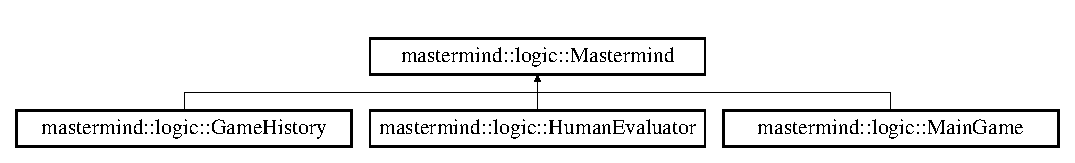
\includegraphics[height=1.736434cm]{classmastermind_1_1logic_1_1_mastermind}
\end{center}
\end{figure}
\subsection*{Public Member Functions}
\begin{DoxyCompactItemize}
\item 
\hyperlink{classmastermind_1_1logic_1_1_mastermind_a386b9f51c21ab36c651f86d1671eccfd}{Mastermind} (uint32\+\_\+t \hyperlink{classmastermind_1_1logic_1_1_mastermind_ac25c65d6c3b258154b632e5edb77fdb7}{max\+\_\+moves}=\hyperlink{classmastermind_1_1logic_1_1_mastermind_a1b389e8f4829939f8fd49e093cb9868b}{D\+E\+F\+A\+U\+L\+T\+\_\+\+M\+A\+X\+\_\+\+M\+O\+V\+ES}, uint32\+\_\+t \hyperlink{classmastermind_1_1logic_1_1_mastermind_a19f901a04d6175f6437b89cd3600c338}{slot\+\_\+count}=\hyperlink{classmastermind_1_1logic_1_1_mastermind_a27d7dbfa1b75744f4b8378e7faaec0af}{D\+E\+F\+A\+U\+L\+T\+\_\+\+S\+L\+O\+T\+\_\+\+C\+O\+U\+NT}, uint32\+\_\+t \hyperlink{classmastermind_1_1logic_1_1_mastermind_a6fe199e91d3e00de452087f0aedabeff}{color\+\_\+count}=\hyperlink{classmastermind_1_1logic_1_1_mastermind_a090907ffd34339289c533fada5bd05c6}{D\+E\+F\+A\+U\+L\+T\+\_\+\+C\+O\+L\+O\+R\+\_\+\+C\+O\+U\+NT})
\item 
uint32\+\_\+t \hyperlink{classmastermind_1_1logic_1_1_mastermind_a7d74266aa973efd0fd9b0cf238c4080f}{get\+Max\+Moves} () const
\begin{DoxyCompactList}\small\item\em Get max moves. \end{DoxyCompactList}\item 
uint32\+\_\+t \hyperlink{classmastermind_1_1logic_1_1_mastermind_a81d6b51ea24fa52073d87d250d7268ff}{get\+Slot\+Count} () const
\begin{DoxyCompactList}\small\item\em Get slot count. \end{DoxyCompactList}\item 
uint32\+\_\+t \hyperlink{classmastermind_1_1logic_1_1_mastermind_ab24668a2fa062cd89a4bd3878b8beef8}{get\+Color\+Count} () const
\begin{DoxyCompactList}\small\item\em Get color count. \end{DoxyCompactList}\item 
uint64\+\_\+t \hyperlink{classmastermind_1_1logic_1_1_mastermind_a75472536b4800a58cfcc47cbe07b02cf}{get\+Code\+Count} () const
\begin{DoxyCompactList}\small\item\em Get code count. \end{DoxyCompactList}\item 
bool \hyperlink{classmastermind_1_1logic_1_1_mastermind_a97247d26b2896c78711cef22611a009b}{is\+Win\+Stick} (const \hyperlink{classmastermind_1_1logic_1_1_black_and_white}{Black\+And\+White} \&bw) const
\end{DoxyCompactItemize}
\subsection*{Static Public Attributes}
\begin{DoxyCompactItemize}
\item 
static constexpr uint32\+\_\+t \hyperlink{classmastermind_1_1logic_1_1_mastermind_a1b389e8f4829939f8fd49e093cb9868b}{D\+E\+F\+A\+U\+L\+T\+\_\+\+M\+A\+X\+\_\+\+M\+O\+V\+ES} = 7
\begin{DoxyCompactList}\small\item\em Maximum moves allowed until game finished. \end{DoxyCompactList}\item 
static constexpr uint32\+\_\+t \hyperlink{classmastermind_1_1logic_1_1_mastermind_a27d7dbfa1b75744f4b8378e7faaec0af}{D\+E\+F\+A\+U\+L\+T\+\_\+\+S\+L\+O\+T\+\_\+\+C\+O\+U\+NT} = 4
\begin{DoxyCompactList}\small\item\em Amount of slots for colors. \end{DoxyCompactList}\item 
static constexpr uint32\+\_\+t \hyperlink{classmastermind_1_1logic_1_1_mastermind_a090907ffd34339289c533fada5bd05c6}{D\+E\+F\+A\+U\+L\+T\+\_\+\+C\+O\+L\+O\+R\+\_\+\+C\+O\+U\+NT} = 6
\begin{DoxyCompactList}\small\item\em Amount of available colors. \end{DoxyCompactList}\end{DoxyCompactItemize}
\subsection*{Private Attributes}
\begin{DoxyCompactItemize}
\item 
const uint32\+\_\+t \hyperlink{classmastermind_1_1logic_1_1_mastermind_ac25c65d6c3b258154b632e5edb77fdb7}{max\+\_\+moves}
\begin{DoxyCompactList}\small\item\em Maximum moves allowed until game finished. \end{DoxyCompactList}\item 
const uint32\+\_\+t \hyperlink{classmastermind_1_1logic_1_1_mastermind_a19f901a04d6175f6437b89cd3600c338}{slot\+\_\+count}
\begin{DoxyCompactList}\small\item\em Amount of slots for colors. \end{DoxyCompactList}\item 
const uint32\+\_\+t \hyperlink{classmastermind_1_1logic_1_1_mastermind_a6fe199e91d3e00de452087f0aedabeff}{color\+\_\+count}
\begin{DoxyCompactList}\small\item\em Amount of available colors. \end{DoxyCompactList}\item 
const uint64\+\_\+t \hyperlink{classmastermind_1_1logic_1_1_mastermind_a66141ba1e71164c2a9c19fbf5d9a6f65}{code\+\_\+count}
\begin{DoxyCompactList}\small\item\em Amount of possible codes. \end{DoxyCompactList}\end{DoxyCompactItemize}


\subsection{Detailed Description}
Class for important global game values. 

\subsection{Constructor \& Destructor Documentation}
\hypertarget{classmastermind_1_1logic_1_1_mastermind_a386b9f51c21ab36c651f86d1671eccfd}{}\label{classmastermind_1_1logic_1_1_mastermind_a386b9f51c21ab36c651f86d1671eccfd} 
\index{mastermind\+::logic\+::\+Mastermind@{mastermind\+::logic\+::\+Mastermind}!Mastermind@{Mastermind}}
\index{Mastermind@{Mastermind}!mastermind\+::logic\+::\+Mastermind@{mastermind\+::logic\+::\+Mastermind}}
\subsubsection{\texorpdfstring{Mastermind()}{Mastermind()}}
{\footnotesize\ttfamily mastermind\+::logic\+::\+Mastermind\+::\+Mastermind (\begin{DoxyParamCaption}\item[{uint32\+\_\+t}]{max\+\_\+moves = {\ttfamily \hyperlink{classmastermind_1_1logic_1_1_mastermind_a1b389e8f4829939f8fd49e093cb9868b}{D\+E\+F\+A\+U\+L\+T\+\_\+\+M\+A\+X\+\_\+\+M\+O\+V\+ES}},  }\item[{uint32\+\_\+t}]{slot\+\_\+count = {\ttfamily \hyperlink{classmastermind_1_1logic_1_1_mastermind_a27d7dbfa1b75744f4b8378e7faaec0af}{D\+E\+F\+A\+U\+L\+T\+\_\+\+S\+L\+O\+T\+\_\+\+C\+O\+U\+NT}},  }\item[{uint32\+\_\+t}]{color\+\_\+count = {\ttfamily \hyperlink{classmastermind_1_1logic_1_1_mastermind_a090907ffd34339289c533fada5bd05c6}{D\+E\+F\+A\+U\+L\+T\+\_\+\+C\+O\+L\+O\+R\+\_\+\+C\+O\+U\+NT}} }\end{DoxyParamCaption})}



\subsection{Member Function Documentation}
\hypertarget{classmastermind_1_1logic_1_1_mastermind_a75472536b4800a58cfcc47cbe07b02cf}{}\label{classmastermind_1_1logic_1_1_mastermind_a75472536b4800a58cfcc47cbe07b02cf} 
\index{mastermind\+::logic\+::\+Mastermind@{mastermind\+::logic\+::\+Mastermind}!get\+Code\+Count@{get\+Code\+Count}}
\index{get\+Code\+Count@{get\+Code\+Count}!mastermind\+::logic\+::\+Mastermind@{mastermind\+::logic\+::\+Mastermind}}
\subsubsection{\texorpdfstring{get\+Code\+Count()}{getCodeCount()}}
{\footnotesize\ttfamily uint64\+\_\+t mastermind\+::logic\+::\+Mastermind\+::get\+Code\+Count (\begin{DoxyParamCaption}{ }\end{DoxyParamCaption}) const}



Get code count. 

\begin{DoxyReturn}{Returns}
code count 
\end{DoxyReturn}
\hypertarget{classmastermind_1_1logic_1_1_mastermind_ab24668a2fa062cd89a4bd3878b8beef8}{}\label{classmastermind_1_1logic_1_1_mastermind_ab24668a2fa062cd89a4bd3878b8beef8} 
\index{mastermind\+::logic\+::\+Mastermind@{mastermind\+::logic\+::\+Mastermind}!get\+Color\+Count@{get\+Color\+Count}}
\index{get\+Color\+Count@{get\+Color\+Count}!mastermind\+::logic\+::\+Mastermind@{mastermind\+::logic\+::\+Mastermind}}
\subsubsection{\texorpdfstring{get\+Color\+Count()}{getColorCount()}}
{\footnotesize\ttfamily uint32\+\_\+t mastermind\+::logic\+::\+Mastermind\+::get\+Color\+Count (\begin{DoxyParamCaption}{ }\end{DoxyParamCaption}) const}



Get color count. 

\begin{DoxyReturn}{Returns}
color count 
\end{DoxyReturn}
\hypertarget{classmastermind_1_1logic_1_1_mastermind_a7d74266aa973efd0fd9b0cf238c4080f}{}\label{classmastermind_1_1logic_1_1_mastermind_a7d74266aa973efd0fd9b0cf238c4080f} 
\index{mastermind\+::logic\+::\+Mastermind@{mastermind\+::logic\+::\+Mastermind}!get\+Max\+Moves@{get\+Max\+Moves}}
\index{get\+Max\+Moves@{get\+Max\+Moves}!mastermind\+::logic\+::\+Mastermind@{mastermind\+::logic\+::\+Mastermind}}
\subsubsection{\texorpdfstring{get\+Max\+Moves()}{getMaxMoves()}}
{\footnotesize\ttfamily uint32\+\_\+t mastermind\+::logic\+::\+Mastermind\+::get\+Max\+Moves (\begin{DoxyParamCaption}{ }\end{DoxyParamCaption}) const}



Get max moves. 

\begin{DoxyReturn}{Returns}
max moves 
\end{DoxyReturn}
\hypertarget{classmastermind_1_1logic_1_1_mastermind_a81d6b51ea24fa52073d87d250d7268ff}{}\label{classmastermind_1_1logic_1_1_mastermind_a81d6b51ea24fa52073d87d250d7268ff} 
\index{mastermind\+::logic\+::\+Mastermind@{mastermind\+::logic\+::\+Mastermind}!get\+Slot\+Count@{get\+Slot\+Count}}
\index{get\+Slot\+Count@{get\+Slot\+Count}!mastermind\+::logic\+::\+Mastermind@{mastermind\+::logic\+::\+Mastermind}}
\subsubsection{\texorpdfstring{get\+Slot\+Count()}{getSlotCount()}}
{\footnotesize\ttfamily uint32\+\_\+t mastermind\+::logic\+::\+Mastermind\+::get\+Slot\+Count (\begin{DoxyParamCaption}{ }\end{DoxyParamCaption}) const}



Get slot count. 

\begin{DoxyReturn}{Returns}
slot count 
\end{DoxyReturn}
\hypertarget{classmastermind_1_1logic_1_1_mastermind_a97247d26b2896c78711cef22611a009b}{}\label{classmastermind_1_1logic_1_1_mastermind_a97247d26b2896c78711cef22611a009b} 
\index{mastermind\+::logic\+::\+Mastermind@{mastermind\+::logic\+::\+Mastermind}!is\+Win\+Stick@{is\+Win\+Stick}}
\index{is\+Win\+Stick@{is\+Win\+Stick}!mastermind\+::logic\+::\+Mastermind@{mastermind\+::logic\+::\+Mastermind}}
\subsubsection{\texorpdfstring{is\+Win\+Stick()}{isWinStick()}}
{\footnotesize\ttfamily bool mastermind\+::logic\+::\+Mastermind\+::is\+Win\+Stick (\begin{DoxyParamCaption}\item[{const \hyperlink{classmastermind_1_1logic_1_1_black_and_white}{Black\+And\+White} \&}]{bw }\end{DoxyParamCaption}) const}



\subsection{Member Data Documentation}
\hypertarget{classmastermind_1_1logic_1_1_mastermind_a66141ba1e71164c2a9c19fbf5d9a6f65}{}\label{classmastermind_1_1logic_1_1_mastermind_a66141ba1e71164c2a9c19fbf5d9a6f65} 
\index{mastermind\+::logic\+::\+Mastermind@{mastermind\+::logic\+::\+Mastermind}!code\+\_\+count@{code\+\_\+count}}
\index{code\+\_\+count@{code\+\_\+count}!mastermind\+::logic\+::\+Mastermind@{mastermind\+::logic\+::\+Mastermind}}
\subsubsection{\texorpdfstring{code\+\_\+count}{code\_count}}
{\footnotesize\ttfamily const uint64\+\_\+t mastermind\+::logic\+::\+Mastermind\+::code\+\_\+count\hspace{0.3cm}{\ttfamily [private]}}



Amount of possible codes. 

\hypertarget{classmastermind_1_1logic_1_1_mastermind_a6fe199e91d3e00de452087f0aedabeff}{}\label{classmastermind_1_1logic_1_1_mastermind_a6fe199e91d3e00de452087f0aedabeff} 
\index{mastermind\+::logic\+::\+Mastermind@{mastermind\+::logic\+::\+Mastermind}!color\+\_\+count@{color\+\_\+count}}
\index{color\+\_\+count@{color\+\_\+count}!mastermind\+::logic\+::\+Mastermind@{mastermind\+::logic\+::\+Mastermind}}
\subsubsection{\texorpdfstring{color\+\_\+count}{color\_count}}
{\footnotesize\ttfamily const uint32\+\_\+t mastermind\+::logic\+::\+Mastermind\+::color\+\_\+count\hspace{0.3cm}{\ttfamily [private]}}



Amount of available colors. 

\hypertarget{classmastermind_1_1logic_1_1_mastermind_a090907ffd34339289c533fada5bd05c6}{}\label{classmastermind_1_1logic_1_1_mastermind_a090907ffd34339289c533fada5bd05c6} 
\index{mastermind\+::logic\+::\+Mastermind@{mastermind\+::logic\+::\+Mastermind}!D\+E\+F\+A\+U\+L\+T\+\_\+\+C\+O\+L\+O\+R\+\_\+\+C\+O\+U\+NT@{D\+E\+F\+A\+U\+L\+T\+\_\+\+C\+O\+L\+O\+R\+\_\+\+C\+O\+U\+NT}}
\index{D\+E\+F\+A\+U\+L\+T\+\_\+\+C\+O\+L\+O\+R\+\_\+\+C\+O\+U\+NT@{D\+E\+F\+A\+U\+L\+T\+\_\+\+C\+O\+L\+O\+R\+\_\+\+C\+O\+U\+NT}!mastermind\+::logic\+::\+Mastermind@{mastermind\+::logic\+::\+Mastermind}}
\subsubsection{\texorpdfstring{D\+E\+F\+A\+U\+L\+T\+\_\+\+C\+O\+L\+O\+R\+\_\+\+C\+O\+U\+NT}{DEFAULT\_COLOR\_COUNT}}
{\footnotesize\ttfamily constexpr uint32\+\_\+t mastermind\+::logic\+::\+Mastermind\+::\+D\+E\+F\+A\+U\+L\+T\+\_\+\+C\+O\+L\+O\+R\+\_\+\+C\+O\+U\+NT = 6\hspace{0.3cm}{\ttfamily [static]}}



Amount of available colors. 

\hypertarget{classmastermind_1_1logic_1_1_mastermind_a1b389e8f4829939f8fd49e093cb9868b}{}\label{classmastermind_1_1logic_1_1_mastermind_a1b389e8f4829939f8fd49e093cb9868b} 
\index{mastermind\+::logic\+::\+Mastermind@{mastermind\+::logic\+::\+Mastermind}!D\+E\+F\+A\+U\+L\+T\+\_\+\+M\+A\+X\+\_\+\+M\+O\+V\+ES@{D\+E\+F\+A\+U\+L\+T\+\_\+\+M\+A\+X\+\_\+\+M\+O\+V\+ES}}
\index{D\+E\+F\+A\+U\+L\+T\+\_\+\+M\+A\+X\+\_\+\+M\+O\+V\+ES@{D\+E\+F\+A\+U\+L\+T\+\_\+\+M\+A\+X\+\_\+\+M\+O\+V\+ES}!mastermind\+::logic\+::\+Mastermind@{mastermind\+::logic\+::\+Mastermind}}
\subsubsection{\texorpdfstring{D\+E\+F\+A\+U\+L\+T\+\_\+\+M\+A\+X\+\_\+\+M\+O\+V\+ES}{DEFAULT\_MAX\_MOVES}}
{\footnotesize\ttfamily constexpr uint32\+\_\+t mastermind\+::logic\+::\+Mastermind\+::\+D\+E\+F\+A\+U\+L\+T\+\_\+\+M\+A\+X\+\_\+\+M\+O\+V\+ES = 7\hspace{0.3cm}{\ttfamily [static]}}



Maximum moves allowed until game finished. 

\hypertarget{classmastermind_1_1logic_1_1_mastermind_a27d7dbfa1b75744f4b8378e7faaec0af}{}\label{classmastermind_1_1logic_1_1_mastermind_a27d7dbfa1b75744f4b8378e7faaec0af} 
\index{mastermind\+::logic\+::\+Mastermind@{mastermind\+::logic\+::\+Mastermind}!D\+E\+F\+A\+U\+L\+T\+\_\+\+S\+L\+O\+T\+\_\+\+C\+O\+U\+NT@{D\+E\+F\+A\+U\+L\+T\+\_\+\+S\+L\+O\+T\+\_\+\+C\+O\+U\+NT}}
\index{D\+E\+F\+A\+U\+L\+T\+\_\+\+S\+L\+O\+T\+\_\+\+C\+O\+U\+NT@{D\+E\+F\+A\+U\+L\+T\+\_\+\+S\+L\+O\+T\+\_\+\+C\+O\+U\+NT}!mastermind\+::logic\+::\+Mastermind@{mastermind\+::logic\+::\+Mastermind}}
\subsubsection{\texorpdfstring{D\+E\+F\+A\+U\+L\+T\+\_\+\+S\+L\+O\+T\+\_\+\+C\+O\+U\+NT}{DEFAULT\_SLOT\_COUNT}}
{\footnotesize\ttfamily constexpr uint32\+\_\+t mastermind\+::logic\+::\+Mastermind\+::\+D\+E\+F\+A\+U\+L\+T\+\_\+\+S\+L\+O\+T\+\_\+\+C\+O\+U\+NT = 4\hspace{0.3cm}{\ttfamily [static]}}



Amount of slots for colors. 

\hypertarget{classmastermind_1_1logic_1_1_mastermind_ac25c65d6c3b258154b632e5edb77fdb7}{}\label{classmastermind_1_1logic_1_1_mastermind_ac25c65d6c3b258154b632e5edb77fdb7} 
\index{mastermind\+::logic\+::\+Mastermind@{mastermind\+::logic\+::\+Mastermind}!max\+\_\+moves@{max\+\_\+moves}}
\index{max\+\_\+moves@{max\+\_\+moves}!mastermind\+::logic\+::\+Mastermind@{mastermind\+::logic\+::\+Mastermind}}
\subsubsection{\texorpdfstring{max\+\_\+moves}{max\_moves}}
{\footnotesize\ttfamily const uint32\+\_\+t mastermind\+::logic\+::\+Mastermind\+::max\+\_\+moves\hspace{0.3cm}{\ttfamily [private]}}



Maximum moves allowed until game finished. 

\hypertarget{classmastermind_1_1logic_1_1_mastermind_a19f901a04d6175f6437b89cd3600c338}{}\label{classmastermind_1_1logic_1_1_mastermind_a19f901a04d6175f6437b89cd3600c338} 
\index{mastermind\+::logic\+::\+Mastermind@{mastermind\+::logic\+::\+Mastermind}!slot\+\_\+count@{slot\+\_\+count}}
\index{slot\+\_\+count@{slot\+\_\+count}!mastermind\+::logic\+::\+Mastermind@{mastermind\+::logic\+::\+Mastermind}}
\subsubsection{\texorpdfstring{slot\+\_\+count}{slot\_count}}
{\footnotesize\ttfamily const uint32\+\_\+t mastermind\+::logic\+::\+Mastermind\+::slot\+\_\+count\hspace{0.3cm}{\ttfamily [private]}}



Amount of slots for colors. 



The documentation for this class was generated from the following files\+:\begin{DoxyCompactItemize}
\item 
Mastermind\+C\+P\+P\+D\+L\+L/\hyperlink{_mastermind_8h}{Mastermind.\+h}\item 
Mastermind\+C\+P\+P\+D\+L\+L/\hyperlink{_mastermind_8cpp}{Mastermind.\+cpp}\end{DoxyCompactItemize}

\hypertarget{classmastermind_1_1shell_1_1_players}{}\section{mastermind\+:\+:shell\+:\+:Players Class Reference}
\label{classmastermind_1_1shell_1_1_players}\index{mastermind\+::shell\+::\+Players@{mastermind\+::shell\+::\+Players}}


\hyperlink{classmastermind_1_1shell_1_1_players}{Players} of the game.  




{\ttfamily \#include $<$Players.\+h$>$}

\subsection*{Public Member Functions}
\begin{DoxyCompactItemize}
\item 
\hyperlink{classmastermind_1_1shell_1_1_players_a0789193995383df718119738773a4d45}{Players} (I\+Guesser $\ast$g, I\+Evaluator $\ast$e)
\begin{DoxyCompactList}\small\item\em Create \hyperlink{classmastermind_1_1shell_1_1_players}{Players}. \end{DoxyCompactList}\item 
I\+Guesser $\ast$ \hyperlink{classmastermind_1_1shell_1_1_players_a66aa10a32b7469eea4f8668ac995cf73}{get\+Guesser} () const
\begin{DoxyCompactList}\small\item\em Get the guesser. \end{DoxyCompactList}\item 
I\+Evaluator $\ast$ \hyperlink{classmastermind_1_1shell_1_1_players_ad79169b7a2096cac0b161d6ed015023f}{get\+Evaluator} () const
\begin{DoxyCompactList}\small\item\em Get the evaluator. \end{DoxyCompactList}\end{DoxyCompactItemize}


\subsection{Detailed Description}
\hyperlink{classmastermind_1_1shell_1_1_players}{Players} of the game. 

\subsection{Constructor \& Destructor Documentation}
\hypertarget{classmastermind_1_1shell_1_1_players_a0789193995383df718119738773a4d45}{}\label{classmastermind_1_1shell_1_1_players_a0789193995383df718119738773a4d45} 
\index{mastermind\+::shell\+::\+Players@{mastermind\+::shell\+::\+Players}!Players@{Players}}
\index{Players@{Players}!mastermind\+::shell\+::\+Players@{mastermind\+::shell\+::\+Players}}
\subsubsection{\texorpdfstring{Players()}{Players()}}
{\footnotesize\ttfamily mastermind\+::shell\+::\+Players\+::\+Players (\begin{DoxyParamCaption}\item[{I\+Guesser $\ast$}]{g,  }\item[{I\+Evaluator $\ast$}]{e }\end{DoxyParamCaption})\hspace{0.3cm}{\ttfamily [inline]}}



Create \hyperlink{classmastermind_1_1shell_1_1_players}{Players}. 


\begin{DoxyParams}{Parameters}
{\em g} & the guesser \\
\hline
{\em e} & the evaluator \\
\hline
\end{DoxyParams}


\subsection{Member Function Documentation}
\hypertarget{classmastermind_1_1shell_1_1_players_ad79169b7a2096cac0b161d6ed015023f}{}\label{classmastermind_1_1shell_1_1_players_ad79169b7a2096cac0b161d6ed015023f} 
\index{mastermind\+::shell\+::\+Players@{mastermind\+::shell\+::\+Players}!get\+Evaluator@{get\+Evaluator}}
\index{get\+Evaluator@{get\+Evaluator}!mastermind\+::shell\+::\+Players@{mastermind\+::shell\+::\+Players}}
\subsubsection{\texorpdfstring{get\+Evaluator()}{getEvaluator()}}
{\footnotesize\ttfamily I\+Evaluator$\ast$ mastermind\+::shell\+::\+Players\+::get\+Evaluator (\begin{DoxyParamCaption}{ }\end{DoxyParamCaption}) const\hspace{0.3cm}{\ttfamily [inline]}}



Get the evaluator. 

\begin{DoxyReturn}{Returns}
the evaluator 
\end{DoxyReturn}
\hypertarget{classmastermind_1_1shell_1_1_players_a66aa10a32b7469eea4f8668ac995cf73}{}\label{classmastermind_1_1shell_1_1_players_a66aa10a32b7469eea4f8668ac995cf73} 
\index{mastermind\+::shell\+::\+Players@{mastermind\+::shell\+::\+Players}!get\+Guesser@{get\+Guesser}}
\index{get\+Guesser@{get\+Guesser}!mastermind\+::shell\+::\+Players@{mastermind\+::shell\+::\+Players}}
\subsubsection{\texorpdfstring{get\+Guesser()}{getGuesser()}}
{\footnotesize\ttfamily I\+Guesser$\ast$ mastermind\+::shell\+::\+Players\+::get\+Guesser (\begin{DoxyParamCaption}{ }\end{DoxyParamCaption}) const\hspace{0.3cm}{\ttfamily [inline]}}



Get the guesser. 

\begin{DoxyReturn}{Returns}
the guesser 
\end{DoxyReturn}


The documentation for this class was generated from the following file\+:\begin{DoxyCompactItemize}
\item 
Mastermind\+C\+P\+P\+D\+L\+L/\hyperlink{_players_8h}{Players.\+h}\end{DoxyCompactItemize}

\hypertarget{classmastermind_1_1logic_1_1_read_only_history}{}\section{mastermind\+:\+:logic\+:\+:Read\+Only\+History Class Reference}
\label{classmastermind_1_1logic_1_1_read_only_history}\index{mastermind\+::logic\+::\+Read\+Only\+History@{mastermind\+::logic\+::\+Read\+Only\+History}}


Read-\/only history to ensure invariant of history.  




{\ttfamily \#include $<$Read\+Only\+History.\+h$>$}

\subsection*{Public Member Functions}
\begin{DoxyCompactItemize}
\item 
\hyperlink{classmastermind_1_1logic_1_1_read_only_history_a47c2ea23a91610532e19d1097d98492e}{Read\+Only\+History} (\hyperlink{classmastermind_1_1logic_1_1_game_history}{Game\+History} $\ast$h)
\item 
std\+::wstring \hyperlink{classmastermind_1_1logic_1_1_read_only_history_afb28dfc9cc7b169a7878bd7567979a36}{to\+String} ()
\end{DoxyCompactItemize}


\subsection{Detailed Description}
Read-\/only history to ensure invariant of history. 

\subsection{Constructor \& Destructor Documentation}
\hypertarget{classmastermind_1_1logic_1_1_read_only_history_a47c2ea23a91610532e19d1097d98492e}{}\label{classmastermind_1_1logic_1_1_read_only_history_a47c2ea23a91610532e19d1097d98492e} 
\index{mastermind\+::logic\+::\+Read\+Only\+History@{mastermind\+::logic\+::\+Read\+Only\+History}!Read\+Only\+History@{Read\+Only\+History}}
\index{Read\+Only\+History@{Read\+Only\+History}!mastermind\+::logic\+::\+Read\+Only\+History@{mastermind\+::logic\+::\+Read\+Only\+History}}
\subsubsection{\texorpdfstring{Read\+Only\+History()}{ReadOnlyHistory()}}
{\footnotesize\ttfamily mastermind\+::logic\+::\+Read\+Only\+History\+::\+Read\+Only\+History (\begin{DoxyParamCaption}\item[{\hyperlink{classmastermind_1_1logic_1_1_game_history}{Game\+History} $\ast$}]{h }\end{DoxyParamCaption})}

Create a read-\/only history. 
\begin{DoxyParams}{Parameters}
{\em h} & the base history \\
\hline
\end{DoxyParams}


\subsection{Member Function Documentation}
\hypertarget{classmastermind_1_1logic_1_1_read_only_history_afb28dfc9cc7b169a7878bd7567979a36}{}\label{classmastermind_1_1logic_1_1_read_only_history_afb28dfc9cc7b169a7878bd7567979a36} 
\index{mastermind\+::logic\+::\+Read\+Only\+History@{mastermind\+::logic\+::\+Read\+Only\+History}!to\+String@{to\+String}}
\index{to\+String@{to\+String}!mastermind\+::logic\+::\+Read\+Only\+History@{mastermind\+::logic\+::\+Read\+Only\+History}}
\subsubsection{\texorpdfstring{to\+String()}{toString()}}
{\footnotesize\ttfamily std\+::wstring mastermind\+::logic\+::\+Read\+Only\+History\+::to\+String (\begin{DoxyParamCaption}{ }\end{DoxyParamCaption})}

Get string of this history. \begin{DoxyReturn}{Returns}
the string 
\end{DoxyReturn}


The documentation for this class was generated from the following files\+:\begin{DoxyCompactItemize}
\item 
Mastermind\+C\+P\+P\+D\+L\+L/Read\+Only\+History.\+h\item 
Mastermind\+C\+P\+P\+D\+L\+L/Read\+Only\+History.\+cpp\end{DoxyCompactItemize}

\hypertarget{structmastermind_1_1shell_1_1utilities_1_1reinterpret__caster}{}\section{mastermind\+:\+:shell\+:\+:utilities\+:\+:reinterpret\+\_\+caster$<$ From, To $>$ Struct Template Reference}
\label{structmastermind_1_1shell_1_1utilities_1_1reinterpret__caster}\index{mastermind\+::shell\+::utilities\+::reinterpret\+\_\+caster$<$ From, To $>$@{mastermind\+::shell\+::utilities\+::reinterpret\+\_\+caster$<$ From, To $>$}}


Reinterpreter for list conversions.  




{\ttfamily \#include $<$Utilities.\+h$>$}

\subsection*{Public Member Functions}
\begin{DoxyCompactItemize}
\item 
To $\ast$ \hyperlink{structmastermind_1_1shell_1_1utilities_1_1reinterpret__caster_ad71fd2afb60510914c98f9bc5e004cc0}{operator()} (From $\ast$p)
\end{DoxyCompactItemize}


\subsection{Detailed Description}
\subsubsection*{template$<$typename From, typename To$>$\newline
struct mastermind\+::shell\+::utilities\+::reinterpret\+\_\+caster$<$ From, To $>$}

Reinterpreter for list conversions. 


\begin{DoxyParams}{Parameters}
{\em From} & type to cast from \\
\hline
{\em To} & type to cast to \\
\hline
{\em p} & pointer to cast \\
\hline
\end{DoxyParams}
\begin{DoxyReturn}{Returns}
the casted pointer 
\end{DoxyReturn}


\subsection{Member Function Documentation}
\hypertarget{structmastermind_1_1shell_1_1utilities_1_1reinterpret__caster_ad71fd2afb60510914c98f9bc5e004cc0}{}\label{structmastermind_1_1shell_1_1utilities_1_1reinterpret__caster_ad71fd2afb60510914c98f9bc5e004cc0} 
\index{mastermind\+::shell\+::utilities\+::reinterpret\+\_\+caster@{mastermind\+::shell\+::utilities\+::reinterpret\+\_\+caster}!operator()@{operator()}}
\index{operator()@{operator()}!mastermind\+::shell\+::utilities\+::reinterpret\+\_\+caster@{mastermind\+::shell\+::utilities\+::reinterpret\+\_\+caster}}
\subsubsection{\texorpdfstring{operator()()}{operator()()}}
{\footnotesize\ttfamily template$<$typename From , typename To $>$ \\
To$\ast$ \hyperlink{structmastermind_1_1shell_1_1utilities_1_1reinterpret__caster}{mastermind\+::shell\+::utilities\+::reinterpret\+\_\+caster}$<$ From, To $>$\+::operator() (\begin{DoxyParamCaption}\item[{From $\ast$}]{p }\end{DoxyParamCaption})\hspace{0.3cm}{\ttfamily [inline]}}



The documentation for this struct was generated from the following file\+:\begin{DoxyCompactItemize}
\item 
Mastermind\+C\+P\+P\+D\+L\+L/\hyperlink{_utilities_8h}{Utilities.\+h}\end{DoxyCompactItemize}

\hypertarget{classmastermind_1_1shell_1_1_shell}{}\section{mastermind\+:\+:shell\+:\+:Shell Class Reference}
\label{classmastermind_1_1shell_1_1_shell}\index{mastermind\+::shell\+::\+Shell@{mastermind\+::shell\+::\+Shell}}
Inheritance diagram for mastermind\+:\+:shell\+:\+:Shell\+:\begin{figure}[H]
\begin{center}
\leavevmode
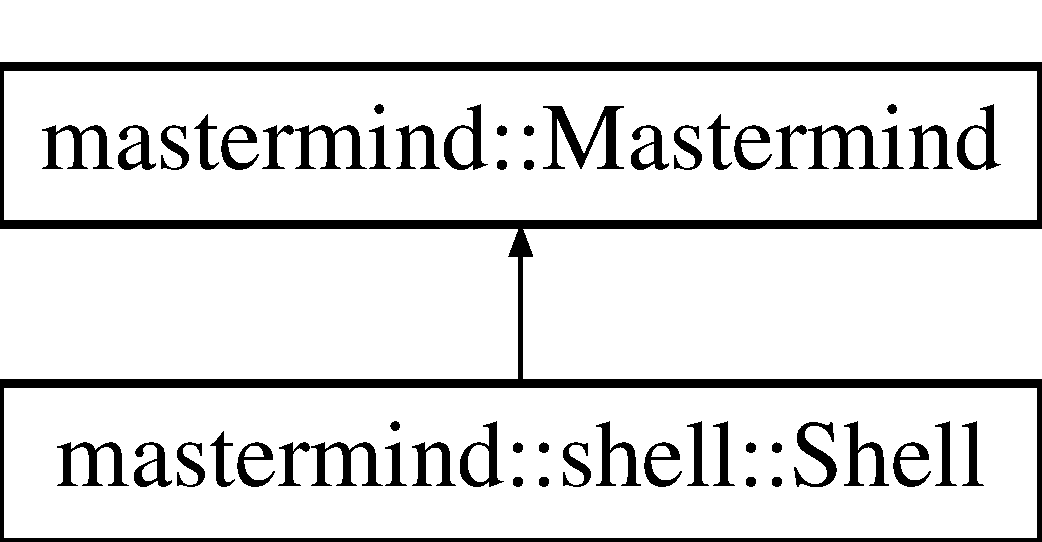
\includegraphics[height=2.000000cm]{classmastermind_1_1shell_1_1_shell}
\end{center}
\end{figure}
\subsection*{Static Public Member Functions}
\begin{DoxyCompactItemize}
\item 
\hypertarget{classmastermind_1_1shell_1_1_shell_aa47488e9975693b33445e871951ec9cd}{}\label{classmastermind_1_1shell_1_1_shell_aa47488e9975693b33445e871951ec9cd} 
static int {\bfseries main} ()
\end{DoxyCompactItemize}
\subsection*{Additional Inherited Members}


The documentation for this class was generated from the following files\+:\begin{DoxyCompactItemize}
\item 
Mastermind\+C\+P\+P\+D\+L\+L/Shell.\+h\item 
Mastermind\+C\+P\+P\+D\+L\+L/Shell.\+cpp\end{DoxyCompactItemize}

\hypertarget{classmastermind_1_1shell_1_1_state}{}\section{mastermind\+:\+:shell\+:\+:State Class Reference}
\label{classmastermind_1_1shell_1_1_state}\index{mastermind\+::shell\+::\+State@{mastermind\+::shell\+::\+State}}


Game state. Class holds the current game state and can be switched here.  




{\ttfamily \#include $<$Requested\+State.\+h$>$}

\subsection*{Public Types}
\begin{DoxyCompactItemize}
\item 
enum \hyperlink{classmastermind_1_1shell_1_1_state_a7667dd4920335355f616e9ffc2793d0b}{Game\+State} \{ \hyperlink{classmastermind_1_1shell_1_1_state_a7667dd4920335355f616e9ffc2793d0ba58938eb78fd16b966e8405452fb2da30}{Game\+State\+::\+H\+U\+M\+A\+N\+\_\+\+G\+U\+E\+S\+S\+ER}, 
\hyperlink{classmastermind_1_1shell_1_1_state_a7667dd4920335355f616e9ffc2793d0ba84b5fa7693dd3d10179d362478250c17}{Game\+State\+::\+C\+O\+M\+P\+U\+T\+E\+R\+\_\+\+G\+U\+E\+S\+S\+ER}
 \}\begin{DoxyCompactList}\small\item\em Available states for games. \end{DoxyCompactList}
\end{DoxyCompactItemize}
\subsection*{Public Member Functions}
\begin{DoxyCompactItemize}
\item 
\hyperlink{classmastermind_1_1shell_1_1_state_a78a389eea152b0305d9600a2cd5decc9}{State} ()
\begin{DoxyCompactList}\small\item\em Create a new state. Initialised to H\+U\+M\+A\+N\+\_\+\+G\+U\+E\+S\+S\+ER. \end{DoxyCompactList}\item 
\hyperlink{classmastermind_1_1shell_1_1_state_acb7ba3f392b85eec1ae099d2c2b34a89}{State} (\hyperlink{classmastermind_1_1shell_1_1_state_a7667dd4920335355f616e9ffc2793d0b}{Game\+State} \hyperlink{classmastermind_1_1shell_1_1_state_a499c4fed4175dd2cc71d325882d3049e}{state})
\begin{DoxyCompactList}\small\item\em Create a new state. \end{DoxyCompactList}\item 
void \hyperlink{classmastermind_1_1shell_1_1_state_ad09ab9698069829ead2841338cf86a6b}{switch\+State} ()
\begin{DoxyCompactList}\small\item\em Switch the state. \end{DoxyCompactList}\item 
\hyperlink{classmastermind_1_1shell_1_1_state_a7667dd4920335355f616e9ffc2793d0b}{Game\+State} \hyperlink{classmastermind_1_1shell_1_1_state_a271f58e7d38180a9c52ff42e2c7de961}{get\+Current\+State} () const
\begin{DoxyCompactList}\small\item\em Get current state. \end{DoxyCompactList}\end{DoxyCompactItemize}
\subsection*{Protected Member Functions}
\begin{DoxyCompactItemize}
\item 
void \hyperlink{classmastermind_1_1shell_1_1_state_a9e4c9895ef013d1d16c1db240ee32344}{switch\+State} (const \hyperlink{classmastermind_1_1shell_1_1_state_a7667dd4920335355f616e9ffc2793d0b}{Game\+State} \&current\+State)
\end{DoxyCompactItemize}
\subsection*{Private Attributes}
\begin{DoxyCompactItemize}
\item 
\hyperlink{classmastermind_1_1shell_1_1_state_a7667dd4920335355f616e9ffc2793d0b}{Game\+State} \hyperlink{classmastermind_1_1shell_1_1_state_a499c4fed4175dd2cc71d325882d3049e}{state}
\end{DoxyCompactItemize}


\subsection{Detailed Description}
Game state. Class holds the current game state and can be switched here. 

\subsection{Member Enumeration Documentation}
\hypertarget{classmastermind_1_1shell_1_1_state_a7667dd4920335355f616e9ffc2793d0b}{}\label{classmastermind_1_1shell_1_1_state_a7667dd4920335355f616e9ffc2793d0b} 
\index{mastermind\+::shell\+::\+State@{mastermind\+::shell\+::\+State}!Game\+State@{Game\+State}}
\index{Game\+State@{Game\+State}!mastermind\+::shell\+::\+State@{mastermind\+::shell\+::\+State}}
\subsubsection{\texorpdfstring{Game\+State}{GameState}}
{\footnotesize\ttfamily enum \hyperlink{classmastermind_1_1shell_1_1_state_a7667dd4920335355f616e9ffc2793d0b}{mastermind\+::shell\+::\+State\+::\+Game\+State}\hspace{0.3cm}{\ttfamily [strong]}}



Available states for games. 

\begin{DoxyEnumFields}{Enumerator}
\raisebox{\heightof{T}}[0pt][0pt]{\index{H\+U\+M\+A\+N\+\_\+\+G\+U\+E\+S\+S\+ER@{H\+U\+M\+A\+N\+\_\+\+G\+U\+E\+S\+S\+ER}!mastermind\+::shell\+::\+State@{mastermind\+::shell\+::\+State}}\index{mastermind\+::shell\+::\+State@{mastermind\+::shell\+::\+State}!H\+U\+M\+A\+N\+\_\+\+G\+U\+E\+S\+S\+ER@{H\+U\+M\+A\+N\+\_\+\+G\+U\+E\+S\+S\+ER}}}\hypertarget{classmastermind_1_1shell_1_1_state_a7667dd4920335355f616e9ffc2793d0ba58938eb78fd16b966e8405452fb2da30}{}\label{classmastermind_1_1shell_1_1_state_a7667dd4920335355f616e9ffc2793d0ba58938eb78fd16b966e8405452fb2da30} 
H\+U\+M\+A\+N\+\_\+\+G\+U\+E\+S\+S\+ER&Human guesser, computer evaluator. \\
\hline

\raisebox{\heightof{T}}[0pt][0pt]{\index{C\+O\+M\+P\+U\+T\+E\+R\+\_\+\+G\+U\+E\+S\+S\+ER@{C\+O\+M\+P\+U\+T\+E\+R\+\_\+\+G\+U\+E\+S\+S\+ER}!mastermind\+::shell\+::\+State@{mastermind\+::shell\+::\+State}}\index{mastermind\+::shell\+::\+State@{mastermind\+::shell\+::\+State}!C\+O\+M\+P\+U\+T\+E\+R\+\_\+\+G\+U\+E\+S\+S\+ER@{C\+O\+M\+P\+U\+T\+E\+R\+\_\+\+G\+U\+E\+S\+S\+ER}}}\hypertarget{classmastermind_1_1shell_1_1_state_a7667dd4920335355f616e9ffc2793d0ba84b5fa7693dd3d10179d362478250c17}{}\label{classmastermind_1_1shell_1_1_state_a7667dd4920335355f616e9ffc2793d0ba84b5fa7693dd3d10179d362478250c17} 
C\+O\+M\+P\+U\+T\+E\+R\+\_\+\+G\+U\+E\+S\+S\+ER&Computer guesser, human evaluator. \\
\hline

\end{DoxyEnumFields}


\subsection{Constructor \& Destructor Documentation}
\hypertarget{classmastermind_1_1shell_1_1_state_a78a389eea152b0305d9600a2cd5decc9}{}\label{classmastermind_1_1shell_1_1_state_a78a389eea152b0305d9600a2cd5decc9} 
\index{mastermind\+::shell\+::\+State@{mastermind\+::shell\+::\+State}!State@{State}}
\index{State@{State}!mastermind\+::shell\+::\+State@{mastermind\+::shell\+::\+State}}
\subsubsection{\texorpdfstring{State()}{State()}\hspace{0.1cm}{\footnotesize\ttfamily [1/2]}}
{\footnotesize\ttfamily mastermind\+::shell\+::\+State\+::\+State (\begin{DoxyParamCaption}{ }\end{DoxyParamCaption})}



Create a new state. Initialised to H\+U\+M\+A\+N\+\_\+\+G\+U\+E\+S\+S\+ER. 

\hypertarget{classmastermind_1_1shell_1_1_state_acb7ba3f392b85eec1ae099d2c2b34a89}{}\label{classmastermind_1_1shell_1_1_state_acb7ba3f392b85eec1ae099d2c2b34a89} 
\index{mastermind\+::shell\+::\+State@{mastermind\+::shell\+::\+State}!State@{State}}
\index{State@{State}!mastermind\+::shell\+::\+State@{mastermind\+::shell\+::\+State}}
\subsubsection{\texorpdfstring{State()}{State()}\hspace{0.1cm}{\footnotesize\ttfamily [2/2]}}
{\footnotesize\ttfamily mastermind\+::shell\+::\+State\+::\+State (\begin{DoxyParamCaption}\item[{\hyperlink{classmastermind_1_1shell_1_1_state_a7667dd4920335355f616e9ffc2793d0b}{Game\+State}}]{state }\end{DoxyParamCaption})}



Create a new state. 


\begin{DoxyParams}{Parameters}
{\em state} & the state to start. \\
\hline
\end{DoxyParams}


\subsection{Member Function Documentation}
\hypertarget{classmastermind_1_1shell_1_1_state_a271f58e7d38180a9c52ff42e2c7de961}{}\label{classmastermind_1_1shell_1_1_state_a271f58e7d38180a9c52ff42e2c7de961} 
\index{mastermind\+::shell\+::\+State@{mastermind\+::shell\+::\+State}!get\+Current\+State@{get\+Current\+State}}
\index{get\+Current\+State@{get\+Current\+State}!mastermind\+::shell\+::\+State@{mastermind\+::shell\+::\+State}}
\subsubsection{\texorpdfstring{get\+Current\+State()}{getCurrentState()}}
{\footnotesize\ttfamily \hyperlink{classmastermind_1_1shell_1_1_state_a7667dd4920335355f616e9ffc2793d0b}{State\+::\+Game\+State} mastermind\+::shell\+::\+State\+::get\+Current\+State (\begin{DoxyParamCaption}{ }\end{DoxyParamCaption}) const}



Get current state. 

\begin{DoxyReturn}{Returns}
the current state 
\end{DoxyReturn}
\hypertarget{classmastermind_1_1shell_1_1_state_ad09ab9698069829ead2841338cf86a6b}{}\label{classmastermind_1_1shell_1_1_state_ad09ab9698069829ead2841338cf86a6b} 
\index{mastermind\+::shell\+::\+State@{mastermind\+::shell\+::\+State}!switch\+State@{switch\+State}}
\index{switch\+State@{switch\+State}!mastermind\+::shell\+::\+State@{mastermind\+::shell\+::\+State}}
\subsubsection{\texorpdfstring{switch\+State()}{switchState()}\hspace{0.1cm}{\footnotesize\ttfamily [1/2]}}
{\footnotesize\ttfamily void mastermind\+::shell\+::\+State\+::switch\+State (\begin{DoxyParamCaption}{ }\end{DoxyParamCaption})}



Switch the state. 

\hypertarget{classmastermind_1_1shell_1_1_state_a9e4c9895ef013d1d16c1db240ee32344}{}\label{classmastermind_1_1shell_1_1_state_a9e4c9895ef013d1d16c1db240ee32344} 
\index{mastermind\+::shell\+::\+State@{mastermind\+::shell\+::\+State}!switch\+State@{switch\+State}}
\index{switch\+State@{switch\+State}!mastermind\+::shell\+::\+State@{mastermind\+::shell\+::\+State}}
\subsubsection{\texorpdfstring{switch\+State()}{switchState()}\hspace{0.1cm}{\footnotesize\ttfamily [2/2]}}
{\footnotesize\ttfamily void mastermind\+::shell\+::\+State\+::switch\+State (\begin{DoxyParamCaption}\item[{const \hyperlink{classmastermind_1_1shell_1_1_state_a7667dd4920335355f616e9ffc2793d0b}{Game\+State} \&}]{current\+State }\end{DoxyParamCaption})\hspace{0.3cm}{\ttfamily [protected]}}



\subsection{Member Data Documentation}
\hypertarget{classmastermind_1_1shell_1_1_state_a499c4fed4175dd2cc71d325882d3049e}{}\label{classmastermind_1_1shell_1_1_state_a499c4fed4175dd2cc71d325882d3049e} 
\index{mastermind\+::shell\+::\+State@{mastermind\+::shell\+::\+State}!state@{state}}
\index{state@{state}!mastermind\+::shell\+::\+State@{mastermind\+::shell\+::\+State}}
\subsubsection{\texorpdfstring{state}{state}}
{\footnotesize\ttfamily \hyperlink{classmastermind_1_1shell_1_1_state_a7667dd4920335355f616e9ffc2793d0b}{Game\+State} mastermind\+::shell\+::\+State\+::state\hspace{0.3cm}{\ttfamily [private]}}



The documentation for this class was generated from the following files\+:\begin{DoxyCompactItemize}
\item 
Mastermind\+C\+P\+P\+D\+L\+L/\hyperlink{_requested_state_8h}{Requested\+State.\+h}\item 
Mastermind\+C\+P\+P\+D\+L\+L/\hyperlink{_requested_state_8cpp}{Requested\+State.\+cpp}\end{DoxyCompactItemize}

\hypertarget{classmastermind_1_1shell_1_1utilities_1_1_utilities}{}\section{mastermind\+:\+:shell\+:\+:utilities\+:\+:Utilities Class Reference}
\label{classmastermind_1_1shell_1_1utilities_1_1_utilities}\index{mastermind\+::shell\+::utilities\+::\+Utilities@{mastermind\+::shell\+::utilities\+::\+Utilities}}


\hyperlink{classmastermind_1_1shell_1_1utilities_1_1_utilities}{Utilities} class.  




{\ttfamily \#include $<$Utilities.\+h$>$}

\subsection*{Static Public Member Functions}
\begin{DoxyCompactItemize}
\item 
static \hyperlink{classmastermind_1_1logic_1_1_color_code}{Color\+Code} $\ast$ \hyperlink{classmastermind_1_1shell_1_1utilities_1_1_utilities_a023c76d90d0588949e26358c3f273219}{create\+Random\+Code} (const uint32\+\_\+t slot\+Count, const uint32\+\_\+t color\+Count)
\begin{DoxyCompactList}\small\item\em Create a random Color\+Code. \end{DoxyCompactList}\item 
static std\+::list$<$ int $\ast$ $>$ \hyperlink{classmastermind_1_1shell_1_1utilities_1_1_utilities_ab364b032c0a68c7a0dbd5696b23d23b0}{parse\+String} (const std\+::wstring \&s)
\begin{DoxyCompactList}\small\item\em Parse a string for numbers. Used for input of Color\+Codes. \end{DoxyCompactList}\item 
static std\+::wstring \hyperlink{classmastermind_1_1shell_1_1utilities_1_1_utilities_a29b0701b6eeea2cc5557da28def33d3e}{create\+Alphabet} (const uint32\+\_\+t slot\+Count)
\begin{DoxyCompactList}\small\item\em Create alphabet string for the representation of the board. \end{DoxyCompactList}\item 
static uint64\+\_\+t \hyperlink{classmastermind_1_1shell_1_1utilities_1_1_utilities_a890a9c41f6a4a13419fb6a7e456bfc4f}{P\+O\+W\+ER} (uint32\+\_\+t lhs, uint32\+\_\+t rhs)
\begin{DoxyCompactList}\small\item\em Calculate power of two uint32\+\_\+t values. \end{DoxyCompactList}\end{DoxyCompactItemize}
\subsection*{Static Protected Member Functions}
\begin{DoxyCompactItemize}
\item 
static void \hyperlink{classmastermind_1_1shell_1_1utilities_1_1_utilities_a9676baba3bcb2d508ccedce50f466a9c}{split} (const std\+::wstring \&s, char delim, std\+::list$<$ std\+::wstring $>$ \&elems)
\item 
static std\+::list$<$ std\+::wstring $>$ \hyperlink{classmastermind_1_1shell_1_1utilities_1_1_utilities_ac053c782cd5669535205daf989e0f695}{split} (const std\+::wstring \&s, char delim)
\begin{DoxyCompactList}\small\item\em Split a string at given delimiters. \end{DoxyCompactList}\end{DoxyCompactItemize}


\subsection{Detailed Description}
\hyperlink{classmastermind_1_1shell_1_1utilities_1_1_utilities}{Utilities} class. 

\subsection{Member Function Documentation}
\hypertarget{classmastermind_1_1shell_1_1utilities_1_1_utilities_a29b0701b6eeea2cc5557da28def33d3e}{}\label{classmastermind_1_1shell_1_1utilities_1_1_utilities_a29b0701b6eeea2cc5557da28def33d3e} 
\index{mastermind\+::shell\+::utilities\+::\+Utilities@{mastermind\+::shell\+::utilities\+::\+Utilities}!create\+Alphabet@{create\+Alphabet}}
\index{create\+Alphabet@{create\+Alphabet}!mastermind\+::shell\+::utilities\+::\+Utilities@{mastermind\+::shell\+::utilities\+::\+Utilities}}
\subsubsection{\texorpdfstring{create\+Alphabet()}{createAlphabet()}}
{\footnotesize\ttfamily std\+::wstring mastermind\+::shell\+::utilities\+::\+Utilities\+::create\+Alphabet (\begin{DoxyParamCaption}\item[{const uint32\+\_\+t}]{slot\+Count }\end{DoxyParamCaption})\hspace{0.3cm}{\ttfamily [static]}}



Create alphabet string for the representation of the board. 

\begin{DoxyReturn}{Returns}
string in the form L\char`\"{}a b c d e\char`\"{} etc. 
\end{DoxyReturn}
\hypertarget{classmastermind_1_1shell_1_1utilities_1_1_utilities_a023c76d90d0588949e26358c3f273219}{}\label{classmastermind_1_1shell_1_1utilities_1_1_utilities_a023c76d90d0588949e26358c3f273219} 
\index{mastermind\+::shell\+::utilities\+::\+Utilities@{mastermind\+::shell\+::utilities\+::\+Utilities}!create\+Random\+Code@{create\+Random\+Code}}
\index{create\+Random\+Code@{create\+Random\+Code}!mastermind\+::shell\+::utilities\+::\+Utilities@{mastermind\+::shell\+::utilities\+::\+Utilities}}
\subsubsection{\texorpdfstring{create\+Random\+Code()}{createRandomCode()}}
{\footnotesize\ttfamily \hyperlink{classmastermind_1_1logic_1_1_color_code}{Color\+Code} $\ast$ mastermind\+::shell\+::utilities\+::\+Utilities\+::create\+Random\+Code (\begin{DoxyParamCaption}\item[{const uint32\+\_\+t}]{slot\+Count,  }\item[{const uint32\+\_\+t}]{color\+Count }\end{DoxyParamCaption})\hspace{0.3cm}{\ttfamily [static]}}



Create a random Color\+Code. 

\begin{DoxyReturn}{Returns}
the Color\+Code 
\end{DoxyReturn}
\hypertarget{classmastermind_1_1shell_1_1utilities_1_1_utilities_ab364b032c0a68c7a0dbd5696b23d23b0}{}\label{classmastermind_1_1shell_1_1utilities_1_1_utilities_ab364b032c0a68c7a0dbd5696b23d23b0} 
\index{mastermind\+::shell\+::utilities\+::\+Utilities@{mastermind\+::shell\+::utilities\+::\+Utilities}!parse\+String@{parse\+String}}
\index{parse\+String@{parse\+String}!mastermind\+::shell\+::utilities\+::\+Utilities@{mastermind\+::shell\+::utilities\+::\+Utilities}}
\subsubsection{\texorpdfstring{parse\+String()}{parseString()}}
{\footnotesize\ttfamily std\+::list$<$ int $\ast$ $>$ mastermind\+::shell\+::utilities\+::\+Utilities\+::parse\+String (\begin{DoxyParamCaption}\item[{const std\+::wstring \&}]{s }\end{DoxyParamCaption})\hspace{0.3cm}{\ttfamily [static]}}



Parse a string for numbers. Used for input of Color\+Codes. 


\begin{DoxyParams}{Parameters}
{\em s} & the string to be parsed \\
\hline
\end{DoxyParams}
\begin{DoxyReturn}{Returns}
the tokens 
\end{DoxyReturn}
\hypertarget{classmastermind_1_1shell_1_1utilities_1_1_utilities_a890a9c41f6a4a13419fb6a7e456bfc4f}{}\label{classmastermind_1_1shell_1_1utilities_1_1_utilities_a890a9c41f6a4a13419fb6a7e456bfc4f} 
\index{mastermind\+::shell\+::utilities\+::\+Utilities@{mastermind\+::shell\+::utilities\+::\+Utilities}!P\+O\+W\+ER@{P\+O\+W\+ER}}
\index{P\+O\+W\+ER@{P\+O\+W\+ER}!mastermind\+::shell\+::utilities\+::\+Utilities@{mastermind\+::shell\+::utilities\+::\+Utilities}}
\subsubsection{\texorpdfstring{P\+O\+W\+E\+R()}{POWER()}}
{\footnotesize\ttfamily uint64\+\_\+t mastermind\+::shell\+::utilities\+::\+Utilities\+::\+P\+O\+W\+ER (\begin{DoxyParamCaption}\item[{uint32\+\_\+t}]{lhs,  }\item[{uint32\+\_\+t}]{rhs }\end{DoxyParamCaption})\hspace{0.3cm}{\ttfamily [static]}}



Calculate power of two uint32\+\_\+t values. 


\begin{DoxyParams}{Parameters}
{\em lhs} & base \\
\hline
{\em rhs} & exponent \\
\hline
\end{DoxyParams}
\begin{DoxyReturn}{Returns}
lhs$^\wedge$rhs 
\end{DoxyReturn}
\hypertarget{classmastermind_1_1shell_1_1utilities_1_1_utilities_a9676baba3bcb2d508ccedce50f466a9c}{}\label{classmastermind_1_1shell_1_1utilities_1_1_utilities_a9676baba3bcb2d508ccedce50f466a9c} 
\index{mastermind\+::shell\+::utilities\+::\+Utilities@{mastermind\+::shell\+::utilities\+::\+Utilities}!split@{split}}
\index{split@{split}!mastermind\+::shell\+::utilities\+::\+Utilities@{mastermind\+::shell\+::utilities\+::\+Utilities}}
\subsubsection{\texorpdfstring{split()}{split()}\hspace{0.1cm}{\footnotesize\ttfamily [1/2]}}
{\footnotesize\ttfamily void mastermind\+::shell\+::utilities\+::\+Utilities\+::split (\begin{DoxyParamCaption}\item[{const std\+::wstring \&}]{s,  }\item[{char}]{delim,  }\item[{std\+::list$<$ std\+::wstring $>$ \&}]{elems }\end{DoxyParamCaption})\hspace{0.3cm}{\ttfamily [static]}, {\ttfamily [protected]}}

\hypertarget{classmastermind_1_1shell_1_1utilities_1_1_utilities_ac053c782cd5669535205daf989e0f695}{}\label{classmastermind_1_1shell_1_1utilities_1_1_utilities_ac053c782cd5669535205daf989e0f695} 
\index{mastermind\+::shell\+::utilities\+::\+Utilities@{mastermind\+::shell\+::utilities\+::\+Utilities}!split@{split}}
\index{split@{split}!mastermind\+::shell\+::utilities\+::\+Utilities@{mastermind\+::shell\+::utilities\+::\+Utilities}}
\subsubsection{\texorpdfstring{split()}{split()}\hspace{0.1cm}{\footnotesize\ttfamily [2/2]}}
{\footnotesize\ttfamily std\+::list$<$ std\+::wstring $>$ mastermind\+::shell\+::utilities\+::\+Utilities\+::split (\begin{DoxyParamCaption}\item[{const std\+::wstring \&}]{s,  }\item[{char}]{delim }\end{DoxyParamCaption})\hspace{0.3cm}{\ttfamily [static]}, {\ttfamily [protected]}}



Split a string at given delimiters. 


\begin{DoxyParams}{Parameters}
{\em s} & the string to be split \\
\hline
{\em delim} & the delimiter \\
\hline
\end{DoxyParams}
\begin{DoxyReturn}{Returns}
the tokens 
\end{DoxyReturn}


The documentation for this class was generated from the following files\+:\begin{DoxyCompactItemize}
\item 
Mastermind\+C\+P\+P\+D\+L\+L/\hyperlink{_utilities_8h}{Utilities.\+h}\item 
Mastermind\+C\+P\+P\+D\+L\+L/\hyperlink{_utilities_8cpp}{Utilities.\+cpp}\end{DoxyCompactItemize}

\chapter{File Documentation}
\input{build-_mastermind_c_p_p-_desktop___qt__5__7__0___m_s_v_c2015__32bit-_debug_2debug_2qrc__qml_8cpp}
\input{build-_mastermind_c_p_p-_desktop___qt__5__7__0___m_s_v_c2015__64bit-_debug_2debug_2qrc__qml_8cpp}
\hypertarget{_mastermind_c_p_p_2_generated_files_2qrc__qml_8cpp}{}\section{Mastermind\+C\+P\+P/\+Generated\+Files/qrc\+\_\+qml.cpp File Reference}
\label{_mastermind_c_p_p_2_generated_files_2qrc__qml_8cpp}\index{Mastermind\+C\+P\+P/\+Generated\+Files/qrc\+\_\+qml.\+cpp@{Mastermind\+C\+P\+P/\+Generated\+Files/qrc\+\_\+qml.\+cpp}}
\subsection*{Macros}
\begin{DoxyCompactItemize}
\item 
\#define \hyperlink{_mastermind_c_p_p_2_generated_files_2qrc__qml_8cpp_afbfc3bb3cd2fa03dd0a3fc36563480d6}{Q\+T\+\_\+\+R\+C\+C\+\_\+\+P\+R\+E\+P\+E\+N\+D\+\_\+\+N\+A\+M\+E\+S\+P\+A\+CE}(name)~name
\item 
\#define \hyperlink{_mastermind_c_p_p_2_generated_files_2qrc__qml_8cpp_a590f80ddb226779f6f432d80438ea190}{Q\+T\+\_\+\+R\+C\+C\+\_\+\+M\+A\+N\+G\+L\+E\+\_\+\+N\+A\+M\+E\+S\+P\+A\+CE}(name)~name
\end{DoxyCompactItemize}
\subsection*{Functions}
\begin{DoxyCompactItemize}
\item 
bool \hyperlink{_mastermind_c_p_p_2_generated_files_2qrc__qml_8cpp_a2ce5a6cde5b318dc75442940471e05f7}{q\+Register\+Resource\+Data} (int, const unsigned char $\ast$, const unsigned char $\ast$, const unsigned char $\ast$)
\item 
bool \hyperlink{_mastermind_c_p_p_2_generated_files_2qrc__qml_8cpp_a54b96c9f44d004fc0ea13bb581f97a71}{q\+Unregister\+Resource\+Data} (int, const unsigned char $\ast$, const unsigned char $\ast$, const unsigned char $\ast$)
\item 
int \hyperlink{_mastermind_c_p_p_2_generated_files_2qrc__qml_8cpp_a590f80ddb226779f6f432d80438ea190}{Q\+T\+\_\+\+R\+C\+C\+\_\+\+M\+A\+N\+G\+L\+E\+\_\+\+N\+A\+M\+E\+S\+P\+A\+CE}() \hyperlink{_mastermind_c_p_p_2_generated_files_2qrc__qml_8cpp_a68995df47257e443e5ab606848a493fc}{q\+Init\+Resources\+\_\+qml} ()
\item 
int \hyperlink{_mastermind_c_p_p_2_generated_files_2qrc__qml_8cpp_a590f80ddb226779f6f432d80438ea190}{Q\+T\+\_\+\+R\+C\+C\+\_\+\+M\+A\+N\+G\+L\+E\+\_\+\+N\+A\+M\+E\+S\+P\+A\+CE}() \hyperlink{_mastermind_c_p_p_2_generated_files_2qrc__qml_8cpp_a83e03aa6ea6d409abf7c8ccfc5746ef0}{q\+Cleanup\+Resources\+\_\+qml} ()
\end{DoxyCompactItemize}
\subsection*{Variables}
\begin{DoxyCompactItemize}
\item 
static const unsigned char \hyperlink{_mastermind_c_p_p_2_generated_files_2qrc__qml_8cpp_a67a985282ed24629b630f624b668842b}{qt\+\_\+resource\+\_\+data} \mbox{[}$\,$\mbox{]}
\item 
static const unsigned char \hyperlink{_mastermind_c_p_p_2_generated_files_2qrc__qml_8cpp_a7931167bf9d7e883e4194a60d031e431}{qt\+\_\+resource\+\_\+name} \mbox{[}$\,$\mbox{]}
\item 
static const unsigned char \hyperlink{_mastermind_c_p_p_2_generated_files_2qrc__qml_8cpp_a37a83d7da2ee18badcd100d79aac64d4}{qt\+\_\+resource\+\_\+struct} \mbox{[}$\,$\mbox{]}
\end{DoxyCompactItemize}


\subsection{Macro Definition Documentation}
\hypertarget{_mastermind_c_p_p_2_generated_files_2qrc__qml_8cpp_a590f80ddb226779f6f432d80438ea190}{}\label{_mastermind_c_p_p_2_generated_files_2qrc__qml_8cpp_a590f80ddb226779f6f432d80438ea190} 
\index{Mastermind\+C\+P\+P/\+Generated\+Files/qrc\+\_\+qml.\+cpp@{Mastermind\+C\+P\+P/\+Generated\+Files/qrc\+\_\+qml.\+cpp}!Q\+T\+\_\+\+R\+C\+C\+\_\+\+M\+A\+N\+G\+L\+E\+\_\+\+N\+A\+M\+E\+S\+P\+A\+CE@{Q\+T\+\_\+\+R\+C\+C\+\_\+\+M\+A\+N\+G\+L\+E\+\_\+\+N\+A\+M\+E\+S\+P\+A\+CE}}
\index{Q\+T\+\_\+\+R\+C\+C\+\_\+\+M\+A\+N\+G\+L\+E\+\_\+\+N\+A\+M\+E\+S\+P\+A\+CE@{Q\+T\+\_\+\+R\+C\+C\+\_\+\+M\+A\+N\+G\+L\+E\+\_\+\+N\+A\+M\+E\+S\+P\+A\+CE}!Mastermind\+C\+P\+P/\+Generated\+Files/qrc\+\_\+qml.\+cpp@{Mastermind\+C\+P\+P/\+Generated\+Files/qrc\+\_\+qml.\+cpp}}
\subsubsection{\texorpdfstring{Q\+T\+\_\+\+R\+C\+C\+\_\+\+M\+A\+N\+G\+L\+E\+\_\+\+N\+A\+M\+E\+S\+P\+A\+CE}{QT\_RCC\_MANGLE\_NAMESPACE}}
{\footnotesize\ttfamily \#define Q\+T\+\_\+\+R\+C\+C\+\_\+\+M\+A\+N\+G\+L\+E\+\_\+\+N\+A\+M\+E\+S\+P\+A\+CE(\begin{DoxyParamCaption}\item[{}]{name }\end{DoxyParamCaption})~name}

\hypertarget{_mastermind_c_p_p_2_generated_files_2qrc__qml_8cpp_afbfc3bb3cd2fa03dd0a3fc36563480d6}{}\label{_mastermind_c_p_p_2_generated_files_2qrc__qml_8cpp_afbfc3bb3cd2fa03dd0a3fc36563480d6} 
\index{Mastermind\+C\+P\+P/\+Generated\+Files/qrc\+\_\+qml.\+cpp@{Mastermind\+C\+P\+P/\+Generated\+Files/qrc\+\_\+qml.\+cpp}!Q\+T\+\_\+\+R\+C\+C\+\_\+\+P\+R\+E\+P\+E\+N\+D\+\_\+\+N\+A\+M\+E\+S\+P\+A\+CE@{Q\+T\+\_\+\+R\+C\+C\+\_\+\+P\+R\+E\+P\+E\+N\+D\+\_\+\+N\+A\+M\+E\+S\+P\+A\+CE}}
\index{Q\+T\+\_\+\+R\+C\+C\+\_\+\+P\+R\+E\+P\+E\+N\+D\+\_\+\+N\+A\+M\+E\+S\+P\+A\+CE@{Q\+T\+\_\+\+R\+C\+C\+\_\+\+P\+R\+E\+P\+E\+N\+D\+\_\+\+N\+A\+M\+E\+S\+P\+A\+CE}!Mastermind\+C\+P\+P/\+Generated\+Files/qrc\+\_\+qml.\+cpp@{Mastermind\+C\+P\+P/\+Generated\+Files/qrc\+\_\+qml.\+cpp}}
\subsubsection{\texorpdfstring{Q\+T\+\_\+\+R\+C\+C\+\_\+\+P\+R\+E\+P\+E\+N\+D\+\_\+\+N\+A\+M\+E\+S\+P\+A\+CE}{QT\_RCC\_PREPEND\_NAMESPACE}}
{\footnotesize\ttfamily \#define Q\+T\+\_\+\+R\+C\+C\+\_\+\+P\+R\+E\+P\+E\+N\+D\+\_\+\+N\+A\+M\+E\+S\+P\+A\+CE(\begin{DoxyParamCaption}\item[{}]{name }\end{DoxyParamCaption})~name}



\subsection{Function Documentation}
\hypertarget{_mastermind_c_p_p_2_generated_files_2qrc__qml_8cpp_a83e03aa6ea6d409abf7c8ccfc5746ef0}{}\label{_mastermind_c_p_p_2_generated_files_2qrc__qml_8cpp_a83e03aa6ea6d409abf7c8ccfc5746ef0} 
\index{Mastermind\+C\+P\+P/\+Generated\+Files/qrc\+\_\+qml.\+cpp@{Mastermind\+C\+P\+P/\+Generated\+Files/qrc\+\_\+qml.\+cpp}!q\+Cleanup\+Resources\+\_\+qml@{q\+Cleanup\+Resources\+\_\+qml}}
\index{q\+Cleanup\+Resources\+\_\+qml@{q\+Cleanup\+Resources\+\_\+qml}!Mastermind\+C\+P\+P/\+Generated\+Files/qrc\+\_\+qml.\+cpp@{Mastermind\+C\+P\+P/\+Generated\+Files/qrc\+\_\+qml.\+cpp}}
\subsubsection{\texorpdfstring{q\+Cleanup\+Resources\+\_\+qml()}{qCleanupResources\_qml()}}
{\footnotesize\ttfamily int \hyperlink{_mastermind_c_p_p_2_generated_files_2qrc__qml_8cpp_a590f80ddb226779f6f432d80438ea190}{Q\+T\+\_\+\+R\+C\+C\+\_\+\+M\+A\+N\+G\+L\+E\+\_\+\+N\+A\+M\+E\+S\+P\+A\+CE}() q\+Cleanup\+Resources\+\_\+qml (\begin{DoxyParamCaption}{ }\end{DoxyParamCaption})}

\hypertarget{_mastermind_c_p_p_2_generated_files_2qrc__qml_8cpp_a68995df47257e443e5ab606848a493fc}{}\label{_mastermind_c_p_p_2_generated_files_2qrc__qml_8cpp_a68995df47257e443e5ab606848a493fc} 
\index{Mastermind\+C\+P\+P/\+Generated\+Files/qrc\+\_\+qml.\+cpp@{Mastermind\+C\+P\+P/\+Generated\+Files/qrc\+\_\+qml.\+cpp}!q\+Init\+Resources\+\_\+qml@{q\+Init\+Resources\+\_\+qml}}
\index{q\+Init\+Resources\+\_\+qml@{q\+Init\+Resources\+\_\+qml}!Mastermind\+C\+P\+P/\+Generated\+Files/qrc\+\_\+qml.\+cpp@{Mastermind\+C\+P\+P/\+Generated\+Files/qrc\+\_\+qml.\+cpp}}
\subsubsection{\texorpdfstring{q\+Init\+Resources\+\_\+qml()}{qInitResources\_qml()}}
{\footnotesize\ttfamily int \hyperlink{_mastermind_c_p_p_2_generated_files_2qrc__qml_8cpp_a590f80ddb226779f6f432d80438ea190}{Q\+T\+\_\+\+R\+C\+C\+\_\+\+M\+A\+N\+G\+L\+E\+\_\+\+N\+A\+M\+E\+S\+P\+A\+CE}() q\+Init\+Resources\+\_\+qml (\begin{DoxyParamCaption}{ }\end{DoxyParamCaption})}

\hypertarget{_mastermind_c_p_p_2_generated_files_2qrc__qml_8cpp_a2ce5a6cde5b318dc75442940471e05f7}{}\label{_mastermind_c_p_p_2_generated_files_2qrc__qml_8cpp_a2ce5a6cde5b318dc75442940471e05f7} 
\index{Mastermind\+C\+P\+P/\+Generated\+Files/qrc\+\_\+qml.\+cpp@{Mastermind\+C\+P\+P/\+Generated\+Files/qrc\+\_\+qml.\+cpp}!q\+Register\+Resource\+Data@{q\+Register\+Resource\+Data}}
\index{q\+Register\+Resource\+Data@{q\+Register\+Resource\+Data}!Mastermind\+C\+P\+P/\+Generated\+Files/qrc\+\_\+qml.\+cpp@{Mastermind\+C\+P\+P/\+Generated\+Files/qrc\+\_\+qml.\+cpp}}
\subsubsection{\texorpdfstring{q\+Register\+Resource\+Data()}{qRegisterResourceData()}}
{\footnotesize\ttfamily bool q\+Register\+Resource\+Data (\begin{DoxyParamCaption}\item[{int}]{,  }\item[{const unsigned char $\ast$}]{,  }\item[{const unsigned char $\ast$}]{,  }\item[{const unsigned char $\ast$}]{ }\end{DoxyParamCaption})}

\hypertarget{_mastermind_c_p_p_2_generated_files_2qrc__qml_8cpp_a54b96c9f44d004fc0ea13bb581f97a71}{}\label{_mastermind_c_p_p_2_generated_files_2qrc__qml_8cpp_a54b96c9f44d004fc0ea13bb581f97a71} 
\index{Mastermind\+C\+P\+P/\+Generated\+Files/qrc\+\_\+qml.\+cpp@{Mastermind\+C\+P\+P/\+Generated\+Files/qrc\+\_\+qml.\+cpp}!q\+Unregister\+Resource\+Data@{q\+Unregister\+Resource\+Data}}
\index{q\+Unregister\+Resource\+Data@{q\+Unregister\+Resource\+Data}!Mastermind\+C\+P\+P/\+Generated\+Files/qrc\+\_\+qml.\+cpp@{Mastermind\+C\+P\+P/\+Generated\+Files/qrc\+\_\+qml.\+cpp}}
\subsubsection{\texorpdfstring{q\+Unregister\+Resource\+Data()}{qUnregisterResourceData()}}
{\footnotesize\ttfamily bool q\+Unregister\+Resource\+Data (\begin{DoxyParamCaption}\item[{int}]{,  }\item[{const unsigned char $\ast$}]{,  }\item[{const unsigned char $\ast$}]{,  }\item[{const unsigned char $\ast$}]{ }\end{DoxyParamCaption})}



\subsection{Variable Documentation}
\hypertarget{_mastermind_c_p_p_2_generated_files_2qrc__qml_8cpp_a67a985282ed24629b630f624b668842b}{}\label{_mastermind_c_p_p_2_generated_files_2qrc__qml_8cpp_a67a985282ed24629b630f624b668842b} 
\index{Mastermind\+C\+P\+P/\+Generated\+Files/qrc\+\_\+qml.\+cpp@{Mastermind\+C\+P\+P/\+Generated\+Files/qrc\+\_\+qml.\+cpp}!qt\+\_\+resource\+\_\+data@{qt\+\_\+resource\+\_\+data}}
\index{qt\+\_\+resource\+\_\+data@{qt\+\_\+resource\+\_\+data}!Mastermind\+C\+P\+P/\+Generated\+Files/qrc\+\_\+qml.\+cpp@{Mastermind\+C\+P\+P/\+Generated\+Files/qrc\+\_\+qml.\+cpp}}
\subsubsection{\texorpdfstring{qt\+\_\+resource\+\_\+data}{qt\_resource\_data}}
{\footnotesize\ttfamily const unsigned char qt\+\_\+resource\+\_\+data\mbox{[}$\,$\mbox{]}\hspace{0.3cm}{\ttfamily [static]}}

\hypertarget{_mastermind_c_p_p_2_generated_files_2qrc__qml_8cpp_a7931167bf9d7e883e4194a60d031e431}{}\label{_mastermind_c_p_p_2_generated_files_2qrc__qml_8cpp_a7931167bf9d7e883e4194a60d031e431} 
\index{Mastermind\+C\+P\+P/\+Generated\+Files/qrc\+\_\+qml.\+cpp@{Mastermind\+C\+P\+P/\+Generated\+Files/qrc\+\_\+qml.\+cpp}!qt\+\_\+resource\+\_\+name@{qt\+\_\+resource\+\_\+name}}
\index{qt\+\_\+resource\+\_\+name@{qt\+\_\+resource\+\_\+name}!Mastermind\+C\+P\+P/\+Generated\+Files/qrc\+\_\+qml.\+cpp@{Mastermind\+C\+P\+P/\+Generated\+Files/qrc\+\_\+qml.\+cpp}}
\subsubsection{\texorpdfstring{qt\+\_\+resource\+\_\+name}{qt\_resource\_name}}
{\footnotesize\ttfamily const unsigned char qt\+\_\+resource\+\_\+name\mbox{[}$\,$\mbox{]}\hspace{0.3cm}{\ttfamily [static]}}

{\bfseries Initial value\+:}
\begin{DoxyCode}
= \{
  
  0x0,0xf,
  0x5,0xe3,0xf8,0x3c,
  0x0,0x4d,
  0x0,0x61,0x0,0x69,0x0,0x6e,0x0,0x46,0x0,0x6f,0x0,0x72,0x0,0x6d,0x0,0x2e,0x0,0x75,0x0,0x69,0x0,0x2e,0x0,
      0x71,0x0,0x6d,0x0,0x6c,
    
  0x0,0x8,
  0x8,0x1,0x5a,0x5c,
  0x0,0x6d,
  0x0,0x61,0x0,0x69,0x0,0x6e,0x0,0x2e,0x0,0x71,0x0,0x6d,0x0,0x6c,
  
\}
\end{DoxyCode}
\hypertarget{_mastermind_c_p_p_2_generated_files_2qrc__qml_8cpp_a37a83d7da2ee18badcd100d79aac64d4}{}\label{_mastermind_c_p_p_2_generated_files_2qrc__qml_8cpp_a37a83d7da2ee18badcd100d79aac64d4} 
\index{Mastermind\+C\+P\+P/\+Generated\+Files/qrc\+\_\+qml.\+cpp@{Mastermind\+C\+P\+P/\+Generated\+Files/qrc\+\_\+qml.\+cpp}!qt\+\_\+resource\+\_\+struct@{qt\+\_\+resource\+\_\+struct}}
\index{qt\+\_\+resource\+\_\+struct@{qt\+\_\+resource\+\_\+struct}!Mastermind\+C\+P\+P/\+Generated\+Files/qrc\+\_\+qml.\+cpp@{Mastermind\+C\+P\+P/\+Generated\+Files/qrc\+\_\+qml.\+cpp}}
\subsubsection{\texorpdfstring{qt\+\_\+resource\+\_\+struct}{qt\_resource\_struct}}
{\footnotesize\ttfamily const unsigned char qt\+\_\+resource\+\_\+struct\mbox{[}$\,$\mbox{]}\hspace{0.3cm}{\ttfamily [static]}}

{\bfseries Initial value\+:}
\begin{DoxyCode}
= \{
  
  0x0,0x0,0x0,0x0,0x0,0x2,0x0,0x0,0x0,0x2,0x0,0x0,0x0,0x1,
  
  0x0,0x0,0x0,0x0,0x0,0x0,0x0,0x0,0x0,0x1,0x0,0x0,0x0,0x0,
  
  0x0,0x0,0x0,0x24,0x0,0x0,0x0,0x0,0x0,0x1,0x0,0x0,0x2,0x91,

\}
\end{DoxyCode}

\hypertarget{main_8cpp}{}\section{Mastermind\+C\+P\+P/main.cpp File Reference}
\label{main_8cpp}\index{Mastermind\+C\+P\+P/main.\+cpp@{Mastermind\+C\+P\+P/main.\+cpp}}
{\ttfamily \#include $<$Q\+Gui\+Application$>$}\newline
{\ttfamily \#include $<$Q\+Qml\+Application\+Engine$>$}\newline
\subsection*{Functions}
\begin{DoxyCompactItemize}
\item 
int \hyperlink{main_8cpp_a0ddf1224851353fc92bfbff6f499fa97}{main} (int argc, char $\ast$argv\mbox{[}$\,$\mbox{]})
\end{DoxyCompactItemize}


\subsection{Function Documentation}
\hypertarget{main_8cpp_a0ddf1224851353fc92bfbff6f499fa97}{}\label{main_8cpp_a0ddf1224851353fc92bfbff6f499fa97} 
\index{main.\+cpp@{main.\+cpp}!main@{main}}
\index{main@{main}!main.\+cpp@{main.\+cpp}}
\subsubsection{\texorpdfstring{main()}{main()}}
{\footnotesize\ttfamily int main (\begin{DoxyParamCaption}\item[{int}]{argc,  }\item[{char $\ast$}]{argv\mbox{[}$\,$\mbox{]} }\end{DoxyParamCaption})}


\hypertarget{_a_p_i_8h}{}\section{Mastermind\+C\+P\+P\+D\+L\+L/\+A\+PI.h File Reference}
\label{_a_p_i_8h}\index{Mastermind\+C\+P\+P\+D\+L\+L/\+A\+P\+I.\+h@{Mastermind\+C\+P\+P\+D\+L\+L/\+A\+P\+I.\+h}}
\subsection*{Macros}
\begin{DoxyCompactItemize}
\item 
\#define \hyperlink{_a_p_i_8h_a93b4dd106b2aed3fba0a3197d32d82ae}{M\+A\+S\+T\+E\+R\+M\+I\+N\+D\+C\+P\+P\+D\+L\+L\+\_\+\+A\+PI}~\+\_\+\+\_\+declspec(dllimport)
\end{DoxyCompactItemize}


\subsection{Macro Definition Documentation}
\hypertarget{_a_p_i_8h_a93b4dd106b2aed3fba0a3197d32d82ae}{}\label{_a_p_i_8h_a93b4dd106b2aed3fba0a3197d32d82ae} 
\index{A\+P\+I.\+h@{A\+P\+I.\+h}!M\+A\+S\+T\+E\+R\+M\+I\+N\+D\+C\+P\+P\+D\+L\+L\+\_\+\+A\+PI@{M\+A\+S\+T\+E\+R\+M\+I\+N\+D\+C\+P\+P\+D\+L\+L\+\_\+\+A\+PI}}
\index{M\+A\+S\+T\+E\+R\+M\+I\+N\+D\+C\+P\+P\+D\+L\+L\+\_\+\+A\+PI@{M\+A\+S\+T\+E\+R\+M\+I\+N\+D\+C\+P\+P\+D\+L\+L\+\_\+\+A\+PI}!A\+P\+I.\+h@{A\+P\+I.\+h}}
\subsubsection{\texorpdfstring{M\+A\+S\+T\+E\+R\+M\+I\+N\+D\+C\+P\+P\+D\+L\+L\+\_\+\+A\+PI}{MASTERMINDCPPDLL\_API}}
{\footnotesize\ttfamily \#define M\+A\+S\+T\+E\+R\+M\+I\+N\+D\+C\+P\+P\+D\+L\+L\+\_\+\+A\+PI~\+\_\+\+\_\+declspec(dllimport)}


\hypertarget{_black_and_white_8cpp}{}\section{Mastermind\+C\+P\+P\+D\+L\+L/\+Black\+And\+White.cpp File Reference}
\label{_black_and_white_8cpp}\index{Mastermind\+C\+P\+P\+D\+L\+L/\+Black\+And\+White.\+cpp@{Mastermind\+C\+P\+P\+D\+L\+L/\+Black\+And\+White.\+cpp}}
{\ttfamily \#include \char`\"{}stdafx.\+h\char`\"{}}\newline
{\ttfamily \#include \char`\"{}Black\+And\+White.\+h\char`\"{}}\newline
{\ttfamily \#include $<$cassert$>$}\newline
\subsection*{Namespaces}
\begin{DoxyCompactItemize}
\item 
 \hyperlink{namespacemastermind}{mastermind}
\item 
 \hyperlink{namespacemastermind_1_1logic}{mastermind\+::logic}
\end{DoxyCompactItemize}

\hypertarget{_black_and_white_8h}{}\section{Mastermind\+C\+P\+P\+D\+L\+L/\+Black\+And\+White.h File Reference}
\label{_black_and_white_8h}\index{Mastermind\+C\+P\+P\+D\+L\+L/\+Black\+And\+White.\+h@{Mastermind\+C\+P\+P\+D\+L\+L/\+Black\+And\+White.\+h}}
{\ttfamily \#include \char`\"{}A\+P\+I.\+h\char`\"{}}\newline
{\ttfamily \#include $<$list$>$}\newline
\subsection*{Classes}
\begin{DoxyCompactItemize}
\item 
class \hyperlink{classmastermind_1_1logic_1_1_black_and_white}{mastermind\+::logic\+::\+Black\+And\+White}
\begin{DoxyCompactList}\small\item\em Representation for evaluation sticks. Black sticks show color and position right. White sticks show color right but wrong position. \end{DoxyCompactList}\end{DoxyCompactItemize}
\subsection*{Namespaces}
\begin{DoxyCompactItemize}
\item 
 \hyperlink{namespacemastermind}{mastermind}
\item 
 \hyperlink{namespacemastermind_1_1logic}{mastermind\+::logic}
\end{DoxyCompactItemize}

\hypertarget{_color_8cpp}{}\section{Mastermind\+C\+P\+P\+D\+L\+L/\+Color.cpp File Reference}
\label{_color_8cpp}\index{Mastermind\+C\+P\+P\+D\+L\+L/\+Color.\+cpp@{Mastermind\+C\+P\+P\+D\+L\+L/\+Color.\+cpp}}
{\ttfamily \#include \char`\"{}stdafx.\+h\char`\"{}}\newline
{\ttfamily \#include \char`\"{}Color.\+h\char`\"{}}\newline
{\ttfamily \#include \char`\"{}Color\+R\+G\+B.\+h\char`\"{}}\newline
{\ttfamily \#include \char`\"{}Color\+H\+S\+I.\+h\char`\"{}}\newline
\subsection*{Namespaces}
\begin{DoxyCompactItemize}
\item 
 \hyperlink{namespacemastermind}{mastermind}
\item 
 \hyperlink{namespacemastermind_1_1logic}{mastermind\+::logic}
\end{DoxyCompactItemize}

\hypertarget{_color_8h}{}\section{Mastermind\+C\+P\+P\+D\+L\+L/\+Color.h File Reference}
\label{_color_8h}\index{Mastermind\+C\+P\+P\+D\+L\+L/\+Color.\+h@{Mastermind\+C\+P\+P\+D\+L\+L/\+Color.\+h}}
{\ttfamily \#include \char`\"{}A\+P\+I.\+h\char`\"{}}\newline
\subsection*{Classes}
\begin{DoxyCompactItemize}
\item 
class \hyperlink{classmastermind_1_1logic_1_1_color}{mastermind\+::logic\+::\+Color}
\begin{DoxyCompactList}\small\item\em A color representation. \end{DoxyCompactList}\end{DoxyCompactItemize}
\subsection*{Namespaces}
\begin{DoxyCompactItemize}
\item 
 \hyperlink{namespacemastermind}{mastermind}
\item 
 \hyperlink{namespacemastermind_1_1logic}{mastermind\+::logic}
\end{DoxyCompactItemize}

\hypertarget{_color_code_8cpp}{}\section{Mastermind\+C\+P\+P\+D\+L\+L/\+Color\+Code.cpp File Reference}
\label{_color_code_8cpp}\index{Mastermind\+C\+P\+P\+D\+L\+L/\+Color\+Code.\+cpp@{Mastermind\+C\+P\+P\+D\+L\+L/\+Color\+Code.\+cpp}}
{\ttfamily \#include \char`\"{}stdafx.\+h\char`\"{}}\newline
{\ttfamily \#include \char`\"{}Color\+Code.\+h\char`\"{}}\newline
{\ttfamily \#include $<$stdexcept$>$}\newline
{\ttfamily \#include $<$iterator$>$}\newline
\subsection*{Namespaces}
\begin{DoxyCompactItemize}
\item 
 \hyperlink{namespacemastermind}{mastermind}
\item 
 \hyperlink{namespacemastermind_1_1logic}{mastermind\+::logic}
\end{DoxyCompactItemize}

\hypertarget{_color_code_8h}{}\section{Mastermind\+C\+P\+P\+D\+L\+L/\+Color\+Code.h File Reference}
\label{_color_code_8h}\index{Mastermind\+C\+P\+P\+D\+L\+L/\+Color\+Code.\+h@{Mastermind\+C\+P\+P\+D\+L\+L/\+Color\+Code.\+h}}
{\ttfamily \#include \char`\"{}A\+P\+I.\+h\char`\"{}}\newline
{\ttfamily \#include $<$vector$>$}\newline
{\ttfamily \#include $<$list$>$}\newline
\subsection*{Classes}
\begin{DoxyCompactItemize}
\item 
class \hyperlink{classmastermind_1_1logic_1_1_color_code}{mastermind\+::logic\+::\+Color\+Code}
\begin{DoxyCompactList}\small\item\em Represents one line of the game board. \end{DoxyCompactList}\end{DoxyCompactItemize}
\subsection*{Namespaces}
\begin{DoxyCompactItemize}
\item 
 \hyperlink{namespacemastermind}{mastermind}
\item 
 \hyperlink{namespacemastermind_1_1logic}{mastermind\+::logic}
\end{DoxyCompactItemize}
\subsection*{Typedefs}
\begin{DoxyCompactItemize}
\item 
typedef uint8\+\_\+t \hyperlink{namespacemastermind_1_1logic_aab4e2166db8e8e5dcbed785c7927eca1}{mastermind\+::logic\+::color\+\_\+t}
\end{DoxyCompactItemize}

\hypertarget{_color_h_s_i_8cpp}{}\section{Mastermind\+C\+P\+P\+D\+L\+L/\+Color\+H\+SI.cpp File Reference}
\label{_color_h_s_i_8cpp}\index{Mastermind\+C\+P\+P\+D\+L\+L/\+Color\+H\+S\+I.\+cpp@{Mastermind\+C\+P\+P\+D\+L\+L/\+Color\+H\+S\+I.\+cpp}}
{\ttfamily \#include \char`\"{}stdafx.\+h\char`\"{}}\newline
{\ttfamily \#include \char`\"{}Color\+H\+S\+I.\+h\char`\"{}}\newline
{\ttfamily \#include \char`\"{}Color\+R\+G\+B.\+h\char`\"{}}\newline
\subsection*{Namespaces}
\begin{DoxyCompactItemize}
\item 
 \hyperlink{namespacemastermind}{mastermind}
\item 
 \hyperlink{namespacemastermind_1_1logic}{mastermind\+::logic}
\end{DoxyCompactItemize}

\hypertarget{_color_h_s_i_8h}{}\section{Mastermind\+C\+P\+P\+D\+L\+L/\+Color\+H\+SI.h File Reference}
\label{_color_h_s_i_8h}\index{Mastermind\+C\+P\+P\+D\+L\+L/\+Color\+H\+S\+I.\+h@{Mastermind\+C\+P\+P\+D\+L\+L/\+Color\+H\+S\+I.\+h}}
{\ttfamily \#include \char`\"{}A\+P\+I.\+h\char`\"{}}\newline
{\ttfamily \#include \char`\"{}Color.\+h\char`\"{}}\newline
\subsection*{Classes}
\begin{DoxyCompactItemize}
\item 
class \hyperlink{classmastermind_1_1logic_1_1_color_h_s_i}{mastermind\+::logic\+::\+Color\+H\+SI}
\begin{DoxyCompactList}\small\item\em A R\+GB color representation. R\+GB values must be each \mbox{[}0..255\mbox{]}. \end{DoxyCompactList}\end{DoxyCompactItemize}
\subsection*{Namespaces}
\begin{DoxyCompactItemize}
\item 
 \hyperlink{namespacemastermind}{mastermind}
\item 
 \hyperlink{namespacemastermind_1_1logic}{mastermind\+::logic}
\end{DoxyCompactItemize}

\hypertarget{_color_r_g_b_8cpp}{}\section{Mastermind\+C\+P\+P\+D\+L\+L/\+Color\+R\+GB.cpp File Reference}
\label{_color_r_g_b_8cpp}\index{Mastermind\+C\+P\+P\+D\+L\+L/\+Color\+R\+G\+B.\+cpp@{Mastermind\+C\+P\+P\+D\+L\+L/\+Color\+R\+G\+B.\+cpp}}
{\ttfamily \#include \char`\"{}stdafx.\+h\char`\"{}}\newline
{\ttfamily \#include \char`\"{}Color\+R\+G\+B.\+h\char`\"{}}\newline
\subsection*{Namespaces}
\begin{DoxyCompactItemize}
\item 
 \hyperlink{namespacemastermind}{mastermind}
\item 
 \hyperlink{namespacemastermind_1_1logic}{mastermind\+::logic}
\end{DoxyCompactItemize}

\hypertarget{_color_r_g_b_8h}{}\section{Mastermind\+C\+P\+P\+D\+L\+L/\+Color\+R\+GB.h File Reference}
\label{_color_r_g_b_8h}\index{Mastermind\+C\+P\+P\+D\+L\+L/\+Color\+R\+G\+B.\+h@{Mastermind\+C\+P\+P\+D\+L\+L/\+Color\+R\+G\+B.\+h}}
{\ttfamily \#include \char`\"{}A\+P\+I.\+h\char`\"{}}\newline
{\ttfamily \#include \char`\"{}Color.\+h\char`\"{}}\newline
\subsection*{Classes}
\begin{DoxyCompactItemize}
\item 
class \hyperlink{classmastermind_1_1logic_1_1_color_r_g_b}{mastermind\+::logic\+::\+Color\+R\+GB}
\begin{DoxyCompactList}\small\item\em A R\+GB color representation. R\+GB values must be each \mbox{[}0..255\mbox{]}. \end{DoxyCompactList}\end{DoxyCompactItemize}
\subsection*{Namespaces}
\begin{DoxyCompactItemize}
\item 
 \hyperlink{namespacemastermind}{mastermind}
\item 
 \hyperlink{namespacemastermind_1_1logic}{mastermind\+::logic}
\end{DoxyCompactItemize}

\hypertarget{_computer_evaluator_8cpp}{}\section{Mastermind\+C\+P\+P\+D\+L\+L/\+Computer\+Evaluator.cpp File Reference}
\label{_computer_evaluator_8cpp}\index{Mastermind\+C\+P\+P\+D\+L\+L/\+Computer\+Evaluator.\+cpp@{Mastermind\+C\+P\+P\+D\+L\+L/\+Computer\+Evaluator.\+cpp}}
{\ttfamily \#include \char`\"{}stdafx.\+h\char`\"{}}\newline
{\ttfamily \#include \char`\"{}Computer\+Evaluator.\+h\char`\"{}}\newline
\subsection*{Namespaces}
\begin{DoxyCompactItemize}
\item 
 \hyperlink{namespacemastermind}{mastermind}
\item 
 \hyperlink{namespacemastermind_1_1logic}{mastermind\+::logic}
\end{DoxyCompactItemize}

\hypertarget{_computer_evaluator_8h}{}\section{Mastermind\+C\+P\+P\+D\+L\+L/\+Computer\+Evaluator.h File Reference}
\label{_computer_evaluator_8h}\index{Mastermind\+C\+P\+P\+D\+L\+L/\+Computer\+Evaluator.\+h@{Mastermind\+C\+P\+P\+D\+L\+L/\+Computer\+Evaluator.\+h}}
{\ttfamily \#include \char`\"{}A\+P\+I.\+h\char`\"{}}\newline
{\ttfamily \#include \char`\"{}Mastermind.\+h\char`\"{}}\newline
{\ttfamily \#include \char`\"{}I\+Evaluator.\+h\char`\"{}}\newline
\subsection*{Classes}
\begin{DoxyCompactItemize}
\item 
class \hyperlink{classmastermind_1_1logic_1_1_computer_evaluator}{mastermind\+::logic\+::\+Computer\+Evaluator}
\begin{DoxyCompactList}\small\item\em Evaluator which automatically evaluates the \hyperlink{classmastermind_1_1logic_1_1_color_code}{Color\+Code} given to a solution. \end{DoxyCompactList}\end{DoxyCompactItemize}
\subsection*{Namespaces}
\begin{DoxyCompactItemize}
\item 
 \hyperlink{namespacemastermind}{mastermind}
\item 
 \hyperlink{namespacemastermind_1_1logic}{mastermind\+::logic}
\end{DoxyCompactItemize}

\hypertarget{_computer_guesser_8cpp}{}\section{Mastermind\+C\+P\+P\+D\+L\+L/\+Computer\+Guesser.cpp File Reference}
\label{_computer_guesser_8cpp}\index{Mastermind\+C\+P\+P\+D\+L\+L/\+Computer\+Guesser.\+cpp@{Mastermind\+C\+P\+P\+D\+L\+L/\+Computer\+Guesser.\+cpp}}
{\ttfamily \#include \char`\"{}stdafx.\+h\char`\"{}}\newline
{\ttfamily \#include \char`\"{}Computer\+Guesser.\+h\char`\"{}}\newline
{\ttfamily \#include \char`\"{}Computer\+Evaluator.\+h\char`\"{}}\newline
{\ttfamily \#include \char`\"{}Utilities.\+h\char`\"{}}\newline
\subsection*{Namespaces}
\begin{DoxyCompactItemize}
\item 
 \hyperlink{namespacemastermind}{mastermind}
\item 
 \hyperlink{namespacemastermind_1_1logic}{mastermind\+::logic}
\end{DoxyCompactItemize}

\hypertarget{_computer_guesser_8h}{}\section{Mastermind\+C\+P\+P\+D\+L\+L/\+Computer\+Guesser.h File Reference}
\label{_computer_guesser_8h}\index{Mastermind\+C\+P\+P\+D\+L\+L/\+Computer\+Guesser.\+h@{Mastermind\+C\+P\+P\+D\+L\+L/\+Computer\+Guesser.\+h}}
{\ttfamily \#include \char`\"{}A\+P\+I.\+h\char`\"{}}\newline
{\ttfamily \#include \char`\"{}I\+Guesser.\+h\char`\"{}}\newline
{\ttfamily \#include \char`\"{}Mastermind.\+h\char`\"{}}\newline
{\ttfamily \#include $<$list$>$}\newline
\subsection*{Classes}
\begin{DoxyCompactItemize}
\item 
class \hyperlink{classmastermind_1_1logic_1_1_computer_guesser}{mastermind\+::logic\+::\+Computer\+Guesser}
\begin{DoxyCompactList}\small\item\em A computer guesser. Uses a heuristic to find a solution. All possibilities are calculated and after each evaluation impossible solutions will be removed. \end{DoxyCompactList}\end{DoxyCompactItemize}
\subsection*{Namespaces}
\begin{DoxyCompactItemize}
\item 
 \hyperlink{namespacemastermind}{mastermind}
\item 
 \hyperlink{namespacemastermind_1_1logic}{mastermind\+::logic}
\end{DoxyCompactItemize}

\hypertarget{dllmain_8cpp}{}\section{Mastermind\+C\+P\+P\+D\+L\+L/dllmain.cpp File Reference}
\label{dllmain_8cpp}\index{Mastermind\+C\+P\+P\+D\+L\+L/dllmain.\+cpp@{Mastermind\+C\+P\+P\+D\+L\+L/dllmain.\+cpp}}
{\ttfamily \#include \char`\"{}stdafx.\+h\char`\"{}}\newline
\subsection*{Functions}
\begin{DoxyCompactItemize}
\item 
B\+O\+OL A\+P\+I\+E\+N\+T\+RY \hyperlink{dllmain_8cpp_a26e64fb39b69bcd9d1274d279f1561b9}{Dll\+Main} (H\+M\+O\+D\+U\+LE h\+Module, D\+W\+O\+RD ul\+\_\+reason\+\_\+for\+\_\+call, L\+P\+V\+O\+ID lp\+Reserved)
\end{DoxyCompactItemize}


\subsection{Function Documentation}
\hypertarget{dllmain_8cpp_a26e64fb39b69bcd9d1274d279f1561b9}{}\label{dllmain_8cpp_a26e64fb39b69bcd9d1274d279f1561b9} 
\index{dllmain.\+cpp@{dllmain.\+cpp}!Dll\+Main@{Dll\+Main}}
\index{Dll\+Main@{Dll\+Main}!dllmain.\+cpp@{dllmain.\+cpp}}
\subsubsection{\texorpdfstring{Dll\+Main()}{DllMain()}}
{\footnotesize\ttfamily B\+O\+OL A\+P\+I\+E\+N\+T\+RY Dll\+Main (\begin{DoxyParamCaption}\item[{H\+M\+O\+D\+U\+LE}]{h\+Module,  }\item[{D\+W\+O\+RD}]{ul\+\_\+reason\+\_\+for\+\_\+call,  }\item[{L\+P\+V\+O\+ID}]{lp\+Reserved }\end{DoxyParamCaption})}


\hypertarget{_game_history_8cpp}{}\section{Mastermind\+C\+P\+P\+D\+L\+L/\+Game\+History.cpp File Reference}
\label{_game_history_8cpp}\index{Mastermind\+C\+P\+P\+D\+L\+L/\+Game\+History.\+cpp@{Mastermind\+C\+P\+P\+D\+L\+L/\+Game\+History.\+cpp}}
{\ttfamily \#include \char`\"{}stdafx.\+h\char`\"{}}\newline
{\ttfamily \#include \char`\"{}Game\+History.\+h\char`\"{}}\newline
\subsection*{Namespaces}
\begin{DoxyCompactItemize}
\item 
 \hyperlink{namespacemastermind}{mastermind}
\item 
 \hyperlink{namespacemastermind_1_1logic}{mastermind\+::logic}
\end{DoxyCompactItemize}

\hypertarget{_game_history_8h}{}\section{Mastermind\+C\+P\+P\+D\+L\+L/\+Game\+History.h File Reference}
\label{_game_history_8h}\index{Mastermind\+C\+P\+P\+D\+L\+L/\+Game\+History.\+h@{Mastermind\+C\+P\+P\+D\+L\+L/\+Game\+History.\+h}}
{\ttfamily \#include \char`\"{}A\+P\+I.\+h\char`\"{}}\newline
{\ttfamily \#include \char`\"{}Mastermind.\+h\char`\"{}}\newline
{\ttfamily \#include \char`\"{}Color\+Code.\+h\char`\"{}}\newline
{\ttfamily \#include \char`\"{}Black\+And\+White.\+h\char`\"{}}\newline
{\ttfamily \#include $<$list$>$}\newline
\subsection*{Classes}
\begin{DoxyCompactItemize}
\item 
class \hyperlink{classmastermind_1_1logic_1_1_game_history}{mastermind\+::logic\+::\+Game\+History}
\begin{DoxyCompactList}\small\item\em Game History. Saves performed moves, i.\+e. Color\+Codes and Black\+And\+Whites, so the board can be printed. \end{DoxyCompactList}\end{DoxyCompactItemize}
\subsection*{Namespaces}
\begin{DoxyCompactItemize}
\item 
 \hyperlink{namespacemastermind}{mastermind}
\item 
 \hyperlink{namespacemastermind_1_1logic}{mastermind\+::logic}
\end{DoxyCompactItemize}

\hypertarget{_human_evaluator_8cpp}{}\section{Mastermind\+C\+P\+P\+D\+L\+L/\+Human\+Evaluator.cpp File Reference}
\label{_human_evaluator_8cpp}\index{Mastermind\+C\+P\+P\+D\+L\+L/\+Human\+Evaluator.\+cpp@{Mastermind\+C\+P\+P\+D\+L\+L/\+Human\+Evaluator.\+cpp}}
{\ttfamily \#include \char`\"{}stdafx.\+h\char`\"{}}\newline
{\ttfamily \#include \char`\"{}Human\+Evaluator.\+h\char`\"{}}\newline
{\ttfamily \#include \char`\"{}Utilities.\+h\char`\"{}}\newline
{\ttfamily \#include $<$iostream$>$}\newline
\subsection*{Namespaces}
\begin{DoxyCompactItemize}
\item 
 \hyperlink{namespacemastermind}{mastermind}
\item 
 \hyperlink{namespacemastermind_1_1logic}{mastermind\+::logic}
\end{DoxyCompactItemize}

\hypertarget{_human_evaluator_8h}{}\section{Mastermind\+C\+P\+P\+D\+L\+L/\+Human\+Evaluator.h File Reference}
\label{_human_evaluator_8h}\index{Mastermind\+C\+P\+P\+D\+L\+L/\+Human\+Evaluator.\+h@{Mastermind\+C\+P\+P\+D\+L\+L/\+Human\+Evaluator.\+h}}
{\ttfamily \#include \char`\"{}A\+P\+I.\+h\char`\"{}}\newline
{\ttfamily \#include \char`\"{}I\+Evaluator.\+h\char`\"{}}\newline
{\ttfamily \#include \char`\"{}Mastermind.\+h\char`\"{}}\newline
{\ttfamily \#include \char`\"{}Read\+Only\+History.\+h\char`\"{}}\newline
\subsection*{Classes}
\begin{DoxyCompactItemize}
\item 
class \hyperlink{classmastermind_1_1logic_1_1_human_evaluator}{mastermind\+::logic\+::\+Human\+Evaluator}
\begin{DoxyCompactList}\small\item\em A human Evaluator for console. \end{DoxyCompactList}\end{DoxyCompactItemize}
\subsection*{Namespaces}
\begin{DoxyCompactItemize}
\item 
 \hyperlink{namespacemastermind}{mastermind}
\item 
 \hyperlink{namespacemastermind_1_1logic}{mastermind\+::logic}
\end{DoxyCompactItemize}

\hypertarget{_human_guesser_8cpp}{}\section{Mastermind\+C\+P\+P\+D\+L\+L/\+Human\+Guesser.cpp File Reference}
\label{_human_guesser_8cpp}\index{Mastermind\+C\+P\+P\+D\+L\+L/\+Human\+Guesser.\+cpp@{Mastermind\+C\+P\+P\+D\+L\+L/\+Human\+Guesser.\+cpp}}
{\ttfamily \#include \char`\"{}stdafx.\+h\char`\"{}}\newline
{\ttfamily \#include \char`\"{}Human\+Guesser.\+h\char`\"{}}\newline
{\ttfamily \#include \char`\"{}Utilities.\+h\char`\"{}}\newline
{\ttfamily \#include $<$iostream$>$}\newline
\subsection*{Namespaces}
\begin{DoxyCompactItemize}
\item 
 \hyperlink{namespacemastermind}{mastermind}
\item 
 \hyperlink{namespacemastermind_1_1logic}{mastermind\+::logic}
\end{DoxyCompactItemize}

\hypertarget{_human_guesser_8h}{}\section{Mastermind\+C\+P\+P\+D\+L\+L/\+Human\+Guesser.h File Reference}
\label{_human_guesser_8h}\index{Mastermind\+C\+P\+P\+D\+L\+L/\+Human\+Guesser.\+h@{Mastermind\+C\+P\+P\+D\+L\+L/\+Human\+Guesser.\+h}}
{\ttfamily \#include \char`\"{}A\+P\+I.\+h\char`\"{}}\newline
{\ttfamily \#include \char`\"{}I\+Guesser.\+h\char`\"{}}\newline
{\ttfamily \#include \char`\"{}Mastermind.\+h\char`\"{}}\newline
{\ttfamily \#include \char`\"{}Read\+Only\+History.\+h\char`\"{}}\newline
\subsection*{Classes}
\begin{DoxyCompactItemize}
\item 
class \hyperlink{classmastermind_1_1logic_1_1_human_guesser}{mastermind\+::logic\+::\+Human\+Guesser}
\begin{DoxyCompactList}\small\item\em A human guesser for console. \end{DoxyCompactList}\end{DoxyCompactItemize}
\subsection*{Namespaces}
\begin{DoxyCompactItemize}
\item 
 \hyperlink{namespacemastermind}{mastermind}
\item 
 \hyperlink{namespacemastermind_1_1logic}{mastermind\+::logic}
\end{DoxyCompactItemize}

\hypertarget{_i_evaluator_8h}{}\section{Mastermind\+C\+P\+P\+D\+L\+L/\+I\+Evaluator.h File Reference}
\label{_i_evaluator_8h}\index{Mastermind\+C\+P\+P\+D\+L\+L/\+I\+Evaluator.\+h@{Mastermind\+C\+P\+P\+D\+L\+L/\+I\+Evaluator.\+h}}
{\ttfamily \#include \char`\"{}A\+P\+I.\+h\char`\"{}}\newline
{\ttfamily \#include \char`\"{}Color\+Code.\+h\char`\"{}}\newline
{\ttfamily \#include \char`\"{}Black\+And\+White.\+h\char`\"{}}\newline
\subsection*{Classes}
\begin{DoxyCompactItemize}
\item 
class \hyperlink{classmastermind_1_1logic_1_1_i_evaluator}{mastermind\+::logic\+::\+I\+Evaluator}
\begin{DoxyCompactList}\small\item\em Interface for an Evaluator of a \hyperlink{classmastermind_1_1logic_1_1_color_code}{Color\+Code}. This interface class should be abstract however Doxygen has parsing problems then. \end{DoxyCompactList}\end{DoxyCompactItemize}
\subsection*{Namespaces}
\begin{DoxyCompactItemize}
\item 
 \hyperlink{namespacemastermind}{mastermind}
\item 
 \hyperlink{namespacemastermind_1_1logic}{mastermind\+::logic}
\end{DoxyCompactItemize}

\hypertarget{_i_guesser_8h}{}\section{Mastermind\+C\+P\+P\+D\+L\+L/\+I\+Guesser.h File Reference}
\label{_i_guesser_8h}\index{Mastermind\+C\+P\+P\+D\+L\+L/\+I\+Guesser.\+h@{Mastermind\+C\+P\+P\+D\+L\+L/\+I\+Guesser.\+h}}
{\ttfamily \#include \char`\"{}A\+P\+I.\+h\char`\"{}}\newline
{\ttfamily \#include \char`\"{}Color\+Code.\+h\char`\"{}}\newline
{\ttfamily \#include \char`\"{}Black\+And\+White.\+h\char`\"{}}\newline
\subsection*{Classes}
\begin{DoxyCompactItemize}
\item 
class \hyperlink{classmastermind_1_1logic_1_1abstract}{mastermind\+::logic\+::abstract}
\begin{DoxyCompactList}\small\item\em Interface for an Evaluator of a \hyperlink{classmastermind_1_1logic_1_1_color_code}{Color\+Code}. \end{DoxyCompactList}\end{DoxyCompactItemize}
\subsection*{Namespaces}
\begin{DoxyCompactItemize}
\item 
 \hyperlink{namespacemastermind}{mastermind}
\item 
 \hyperlink{namespacemastermind_1_1logic}{mastermind\+::logic}
\end{DoxyCompactItemize}

\hypertarget{_main_game_8cpp}{}\section{Mastermind\+C\+P\+P\+D\+L\+L/\+Main\+Game.cpp File Reference}
\label{_main_game_8cpp}\index{Mastermind\+C\+P\+P\+D\+L\+L/\+Main\+Game.\+cpp@{Mastermind\+C\+P\+P\+D\+L\+L/\+Main\+Game.\+cpp}}
{\ttfamily \#include \char`\"{}stdafx.\+h\char`\"{}}\newline
{\ttfamily \#include \char`\"{}Main\+Game.\+h\char`\"{}}\newline
\subsection*{Namespaces}
\begin{DoxyCompactItemize}
\item 
 \hyperlink{namespacemastermind}{mastermind}
\item 
 \hyperlink{namespacemastermind_1_1logic}{mastermind\+::logic}
\end{DoxyCompactItemize}

\hypertarget{_main_game_8h}{}\section{Mastermind\+C\+P\+P\+D\+L\+L/\+Main\+Game.h File Reference}
\label{_main_game_8h}\index{Mastermind\+C\+P\+P\+D\+L\+L/\+Main\+Game.\+h@{Mastermind\+C\+P\+P\+D\+L\+L/\+Main\+Game.\+h}}
{\ttfamily \#include \char`\"{}A\+P\+I.\+h\char`\"{}}\newline
{\ttfamily \#include \char`\"{}Mastermind.\+h\char`\"{}}\newline
{\ttfamily \#include \char`\"{}I\+Evaluator.\+h\char`\"{}}\newline
{\ttfamily \#include \char`\"{}I\+Guesser.\+h\char`\"{}}\newline
{\ttfamily \#include \char`\"{}Game\+History.\+h\char`\"{}}\newline
\subsection*{Classes}
\begin{DoxyCompactItemize}
\item 
class \hyperlink{classmastermind_1_1logic_1_1_main_game}{mastermind\+::logic\+::\+Main\+Game}
\begin{DoxyCompactList}\small\item\em The Game. Game logic is in here. No in and output. Works only with the interfaces of \hyperlink{classmastermind_1_1logic_1_1_i_evaluator}{I\+Evaluator} and \hyperlink{classmastermind_1_1logic_1_1_i_guesser}{I\+Guesser}. \end{DoxyCompactList}\end{DoxyCompactItemize}
\subsection*{Namespaces}
\begin{DoxyCompactItemize}
\item 
 \hyperlink{namespacemastermind}{mastermind}
\item 
 \hyperlink{namespacemastermind_1_1logic}{mastermind\+::logic}
\end{DoxyCompactItemize}

\hypertarget{_mastermind_8cpp}{}\section{Mastermind\+C\+P\+P\+D\+L\+L/\+Mastermind.cpp File Reference}
\label{_mastermind_8cpp}\index{Mastermind\+C\+P\+P\+D\+L\+L/\+Mastermind.\+cpp@{Mastermind\+C\+P\+P\+D\+L\+L/\+Mastermind.\+cpp}}
{\ttfamily \#include \char`\"{}stdafx.\+h\char`\"{}}\newline
{\ttfamily \#include \char`\"{}Mastermind.\+h\char`\"{}}\newline
{\ttfamily \#include \char`\"{}Utilities.\+h\char`\"{}}\newline
\subsection*{Namespaces}
\begin{DoxyCompactItemize}
\item 
 \hyperlink{namespacemastermind}{mastermind}
\item 
 \hyperlink{namespacemastermind_1_1logic}{mastermind\+::logic}
\end{DoxyCompactItemize}

\hypertarget{_mastermind_8h}{}\section{Mastermind\+C\+P\+P\+D\+L\+L/\+Mastermind.h File Reference}
\label{_mastermind_8h}\index{Mastermind\+C\+P\+P\+D\+L\+L/\+Mastermind.\+h@{Mastermind\+C\+P\+P\+D\+L\+L/\+Mastermind.\+h}}
{\ttfamily \#include \char`\"{}A\+P\+I.\+h\char`\"{}}\newline
{\ttfamily \#include $<$string$>$}\newline
\subsection*{Classes}
\begin{DoxyCompactItemize}
\item 
class \hyperlink{classmastermind_1_1_mastermind}{mastermind\+::\+Mastermind}
\begin{DoxyCompactList}\small\item\em Class for important global game values. \end{DoxyCompactList}\end{DoxyCompactItemize}
\subsection*{Namespaces}
\begin{DoxyCompactItemize}
\item 
 \hyperlink{namespacemastermind}{mastermind}
\end{DoxyCompactItemize}

\hypertarget{_players_8cpp}{}\section{Mastermind\+C\+P\+P\+D\+L\+L/\+Players.cpp File Reference}
\label{_players_8cpp}\index{Mastermind\+C\+P\+P\+D\+L\+L/\+Players.\+cpp@{Mastermind\+C\+P\+P\+D\+L\+L/\+Players.\+cpp}}
{\ttfamily \#include \char`\"{}stdafx.\+h\char`\"{}}\newline
{\ttfamily \#include \char`\"{}Players.\+h\char`\"{}}\newline
{\ttfamily \#include \char`\"{}Human\+Guesser.\+h\char`\"{}}\newline
{\ttfamily \#include \char`\"{}Human\+Evaluator.\+h\char`\"{}}\newline
{\ttfamily \#include \char`\"{}Computer\+Guesser.\+h\char`\"{}}\newline
{\ttfamily \#include \char`\"{}Computer\+Evaluator.\+h\char`\"{}}\newline
{\ttfamily \#include \char`\"{}Utilities.\+h\char`\"{}}\newline
\subsection*{Namespaces}
\begin{DoxyCompactItemize}
\item 
 \hyperlink{namespacemastermind}{mastermind}
\item 
 \hyperlink{namespacemastermind_1_1shell}{mastermind\+::shell}
\end{DoxyCompactItemize}

\hypertarget{_players_8h}{}\section{Mastermind\+C\+P\+P\+D\+L\+L/\+Players.h File Reference}
\label{_players_8h}\index{Mastermind\+C\+P\+P\+D\+L\+L/\+Players.\+h@{Mastermind\+C\+P\+P\+D\+L\+L/\+Players.\+h}}
{\ttfamily \#include \char`\"{}A\+P\+I.\+h\char`\"{}}\newline
{\ttfamily \#include \char`\"{}I\+Guesser.\+h\char`\"{}}\newline
{\ttfamily \#include \char`\"{}I\+Evaluator.\+h\char`\"{}}\newline
{\ttfamily \#include \char`\"{}Requested\+State.\+h\char`\"{}}\newline
{\ttfamily \#include \char`\"{}Game\+History.\+h\char`\"{}}\newline
{\ttfamily \#include \char`\"{}Human\+Guesser.\+h\char`\"{}}\newline
{\ttfamily \#include \char`\"{}Human\+Evaluator.\+h\char`\"{}}\newline
{\ttfamily \#include \char`\"{}Computer\+Guesser.\+h\char`\"{}}\newline
{\ttfamily \#include \char`\"{}Computer\+Evaluator.\+h\char`\"{}}\newline
{\ttfamily \#include \char`\"{}Utilities.\+h\char`\"{}}\newline
\subsection*{Classes}
\begin{DoxyCompactItemize}
\item 
class \hyperlink{classmastermind_1_1shell_1_1_players}{mastermind\+::shell\+::\+Players}
\begin{DoxyCompactList}\small\item\em \hyperlink{classmastermind_1_1shell_1_1_players}{Players} of the game. \end{DoxyCompactList}\end{DoxyCompactItemize}
\subsection*{Namespaces}
\begin{DoxyCompactItemize}
\item 
 \hyperlink{namespacemastermind}{mastermind}
\item 
 \hyperlink{namespacemastermind_1_1shell}{mastermind\+::shell}
\end{DoxyCompactItemize}
\subsection*{Functions}
\begin{DoxyCompactItemize}
\item 
Players $\ast$ \hyperlink{namespacemastermind_1_1shell_a516fea896c290c75364c483e71389b3d}{mastermind\+::shell\+::get\+Players} (Requested\+State state, Game\+History $\ast$history)
\begin{DoxyCompactList}\small\item\em Get the player objects. Just here are the objects created so the objects are created just in time. (in case someone \char`\"{}switches\char`\"{} pretty often...) \end{DoxyCompactList}\end{DoxyCompactItemize}

\hypertarget{_read_only_history_8cpp}{}\section{Mastermind\+C\+P\+P\+D\+L\+L/\+Read\+Only\+History.cpp File Reference}
\label{_read_only_history_8cpp}\index{Mastermind\+C\+P\+P\+D\+L\+L/\+Read\+Only\+History.\+cpp@{Mastermind\+C\+P\+P\+D\+L\+L/\+Read\+Only\+History.\+cpp}}
{\ttfamily \#include \char`\"{}stdafx.\+h\char`\"{}}\newline
{\ttfamily \#include \char`\"{}Read\+Only\+History.\+h\char`\"{}}\newline
\subsection*{Namespaces}
\begin{DoxyCompactItemize}
\item 
 \hyperlink{namespacemastermind}{mastermind}
\item 
 \hyperlink{namespacemastermind_1_1logic}{mastermind\+::logic}
\end{DoxyCompactItemize}

\hypertarget{_read_only_history_8h}{}\section{Mastermind\+C\+P\+P\+D\+L\+L/\+Read\+Only\+History.h File Reference}
\label{_read_only_history_8h}\index{Mastermind\+C\+P\+P\+D\+L\+L/\+Read\+Only\+History.\+h@{Mastermind\+C\+P\+P\+D\+L\+L/\+Read\+Only\+History.\+h}}
{\ttfamily \#include \char`\"{}A\+P\+I.\+h\char`\"{}}\newline
{\ttfamily \#include \char`\"{}Game\+History.\+h\char`\"{}}\newline
\subsection*{Classes}
\begin{DoxyCompactItemize}
\item 
class \hyperlink{classmastermind_1_1logic_1_1_read_only_history}{mastermind\+::logic\+::\+Read\+Only\+History}
\begin{DoxyCompactList}\small\item\em Read-\/only history to ensure invariant of history. \end{DoxyCompactList}\end{DoxyCompactItemize}
\subsection*{Namespaces}
\begin{DoxyCompactItemize}
\item 
 \hyperlink{namespacemastermind}{mastermind}
\item 
 \hyperlink{namespacemastermind_1_1logic}{mastermind\+::logic}
\end{DoxyCompactItemize}

\hypertarget{_requested_state_8cpp}{}\section{Mastermind\+C\+P\+P\+D\+L\+L/\+Requested\+State.cpp File Reference}
\label{_requested_state_8cpp}\index{Mastermind\+C\+P\+P\+D\+L\+L/\+Requested\+State.\+cpp@{Mastermind\+C\+P\+P\+D\+L\+L/\+Requested\+State.\+cpp}}
{\ttfamily \#include \char`\"{}stdafx.\+h\char`\"{}}\newline
{\ttfamily \#include \char`\"{}Requested\+State.\+h\char`\"{}}\newline
\subsection*{Namespaces}
\begin{DoxyCompactItemize}
\item 
 \hyperlink{namespacemastermind}{mastermind}
\item 
 \hyperlink{namespacemastermind_1_1shell}{mastermind\+::shell}
\end{DoxyCompactItemize}

\hypertarget{_requested_state_8h}{}\section{Mastermind\+C\+P\+P\+D\+L\+L/\+Requested\+State.h File Reference}
\label{_requested_state_8h}\index{Mastermind\+C\+P\+P\+D\+L\+L/\+Requested\+State.\+h@{Mastermind\+C\+P\+P\+D\+L\+L/\+Requested\+State.\+h}}
{\ttfamily \#include $<$stdexcept$>$}\newline
\subsection*{Namespaces}
\begin{DoxyCompactItemize}
\item 
 \hyperlink{namespacemastermind}{mastermind}
\item 
 \hyperlink{namespacemastermind_1_1shell}{mastermind\+::shell}
\end{DoxyCompactItemize}
\subsection*{Enumerations}
\begin{DoxyCompactItemize}
\item 
enum \hyperlink{namespacemastermind_1_1shell_ad060dfaf42b2c0f7827708f0d0046ede}{mastermind\+::shell\+::\+Requested\+State} \{ \hyperlink{namespacemastermind_1_1shell_ad060dfaf42b2c0f7827708f0d0046edeacc5ce9ad68fd8bcf63c6431048467ac2}{mastermind\+::shell\+::\+H\+U\+M\+A\+N\+\_\+\+G\+U\+E\+S\+S\+ER}, 
\hyperlink{namespacemastermind_1_1shell_ad060dfaf42b2c0f7827708f0d0046edea3853901e4a57fe6d139724873c112ed8}{mastermind\+::shell\+::\+C\+O\+M\+P\+U\+T\+E\+R\+\_\+\+G\+U\+E\+S\+S\+ER}
 \}\begin{DoxyCompactList}\small\item\em Available states for games. \end{DoxyCompactList}
\end{DoxyCompactItemize}

\hypertarget{_mastermind_c_p_p_d_l_l_2stdafx_8cpp}{}\section{Mastermind\+C\+P\+P\+D\+L\+L/stdafx.cpp File Reference}
\label{_mastermind_c_p_p_d_l_l_2stdafx_8cpp}\index{Mastermind\+C\+P\+P\+D\+L\+L/stdafx.\+cpp@{Mastermind\+C\+P\+P\+D\+L\+L/stdafx.\+cpp}}
{\ttfamily \#include \char`\"{}stdafx.\+h\char`\"{}}\newline

\hypertarget{_mastermind_shell_2stdafx_8cpp}{}\section{Mastermind\+Shell/stdafx.cpp File Reference}
\label{_mastermind_shell_2stdafx_8cpp}\index{Mastermind\+Shell/stdafx.\+cpp@{Mastermind\+Shell/stdafx.\+cpp}}
{\ttfamily \#include \char`\"{}stdafx.\+h\char`\"{}}\newline

\hypertarget{_unit_test1_2stdafx_8cpp}{}\section{Unit\+Test1/stdafx.cpp File Reference}
\label{_unit_test1_2stdafx_8cpp}\index{Unit\+Test1/stdafx.\+cpp@{Unit\+Test1/stdafx.\+cpp}}
{\ttfamily \#include \char`\"{}stdafx.\+h\char`\"{}}\newline

\hypertarget{_mastermind_c_p_p_d_l_l_2stdafx_8h}{}\section{Mastermind\+C\+P\+P\+D\+L\+L/stdafx.h File Reference}
\label{_mastermind_c_p_p_d_l_l_2stdafx_8h}\index{Mastermind\+C\+P\+P\+D\+L\+L/stdafx.\+h@{Mastermind\+C\+P\+P\+D\+L\+L/stdafx.\+h}}
{\ttfamily \#include \char`\"{}targetver.\+h\char`\"{}}\newline
{\ttfamily \#include $<$windows.\+h$>$}\newline
\subsection*{Macros}
\begin{DoxyCompactItemize}
\item 
\#define \hyperlink{_mastermind_c_p_p_d_l_l_2stdafx_8h_ac7bef5d85e3dcd73eef56ad39ffc84a9}{W\+I\+N32\+\_\+\+L\+E\+A\+N\+\_\+\+A\+N\+D\+\_\+\+M\+E\+AN}
\end{DoxyCompactItemize}


\subsection{Macro Definition Documentation}
\hypertarget{_mastermind_c_p_p_d_l_l_2stdafx_8h_ac7bef5d85e3dcd73eef56ad39ffc84a9}{}\label{_mastermind_c_p_p_d_l_l_2stdafx_8h_ac7bef5d85e3dcd73eef56ad39ffc84a9} 
\index{Mastermind\+C\+P\+P\+D\+L\+L/stdafx.\+h@{Mastermind\+C\+P\+P\+D\+L\+L/stdafx.\+h}!W\+I\+N32\+\_\+\+L\+E\+A\+N\+\_\+\+A\+N\+D\+\_\+\+M\+E\+AN@{W\+I\+N32\+\_\+\+L\+E\+A\+N\+\_\+\+A\+N\+D\+\_\+\+M\+E\+AN}}
\index{W\+I\+N32\+\_\+\+L\+E\+A\+N\+\_\+\+A\+N\+D\+\_\+\+M\+E\+AN@{W\+I\+N32\+\_\+\+L\+E\+A\+N\+\_\+\+A\+N\+D\+\_\+\+M\+E\+AN}!Mastermind\+C\+P\+P\+D\+L\+L/stdafx.\+h@{Mastermind\+C\+P\+P\+D\+L\+L/stdafx.\+h}}
\subsubsection{\texorpdfstring{W\+I\+N32\+\_\+\+L\+E\+A\+N\+\_\+\+A\+N\+D\+\_\+\+M\+E\+AN}{WIN32\_LEAN\_AND\_MEAN}}
{\footnotesize\ttfamily \#define W\+I\+N32\+\_\+\+L\+E\+A\+N\+\_\+\+A\+N\+D\+\_\+\+M\+E\+AN}


\hypertarget{_mastermind_shell_2stdafx_8h}{}\section{Mastermind\+Shell/stdafx.h File Reference}
\label{_mastermind_shell_2stdafx_8h}\index{Mastermind\+Shell/stdafx.\+h@{Mastermind\+Shell/stdafx.\+h}}
{\ttfamily \#include \char`\"{}targetver.\+h\char`\"{}}\newline
{\ttfamily \#include $<$stdio.\+h$>$}\newline
{\ttfamily \#include $<$tchar.\+h$>$}\newline
{\ttfamily \#include $<$cassert$>$}\newline
{\ttfamily \#include $<$stdexcept$>$}\newline
{\ttfamily \#include $<$string$>$}\newline
{\ttfamily \#include $<$iostream$>$}\newline

\hypertarget{_unit_test1_2stdafx_8h}{}\section{Unit\+Test1/stdafx.h File Reference}
\label{_unit_test1_2stdafx_8h}\index{Unit\+Test1/stdafx.\+h@{Unit\+Test1/stdafx.\+h}}
{\ttfamily \#include \char`\"{}targetver.\+h\char`\"{}}\newline
{\ttfamily \#include \char`\"{}Cpp\+Unit\+Test.\+h\char`\"{}}\newline
{\ttfamily \#include $<$cmath$>$}\newline
{\ttfamily \#include $<$vector$>$}\newline
\subsection*{Macros}
\begin{DoxyCompactItemize}
\item 
\#define \hyperlink{_unit_test1_2stdafx_8h_a525335710b53cb064ca56b936120431e}{\+\_\+\+U\+S\+E\+\_\+\+M\+A\+T\+H\+\_\+\+D\+E\+F\+I\+N\+ES}
\end{DoxyCompactItemize}


\subsection{Macro Definition Documentation}
\hypertarget{_unit_test1_2stdafx_8h_a525335710b53cb064ca56b936120431e}{}\label{_unit_test1_2stdafx_8h_a525335710b53cb064ca56b936120431e} 
\index{Unit\+Test1/stdafx.\+h@{Unit\+Test1/stdafx.\+h}!\+\_\+\+U\+S\+E\+\_\+\+M\+A\+T\+H\+\_\+\+D\+E\+F\+I\+N\+ES@{\+\_\+\+U\+S\+E\+\_\+\+M\+A\+T\+H\+\_\+\+D\+E\+F\+I\+N\+ES}}
\index{\+\_\+\+U\+S\+E\+\_\+\+M\+A\+T\+H\+\_\+\+D\+E\+F\+I\+N\+ES@{\+\_\+\+U\+S\+E\+\_\+\+M\+A\+T\+H\+\_\+\+D\+E\+F\+I\+N\+ES}!Unit\+Test1/stdafx.\+h@{Unit\+Test1/stdafx.\+h}}
\subsubsection{\texorpdfstring{\+\_\+\+U\+S\+E\+\_\+\+M\+A\+T\+H\+\_\+\+D\+E\+F\+I\+N\+ES}{\_USE\_MATH\_DEFINES}}
{\footnotesize\ttfamily \#define \+\_\+\+U\+S\+E\+\_\+\+M\+A\+T\+H\+\_\+\+D\+E\+F\+I\+N\+ES}


\hypertarget{_mastermind_c_p_p_d_l_l_2targetver_8h}{}\section{Mastermind\+C\+P\+P\+D\+L\+L/targetver.h File Reference}
\label{_mastermind_c_p_p_d_l_l_2targetver_8h}\index{Mastermind\+C\+P\+P\+D\+L\+L/targetver.\+h@{Mastermind\+C\+P\+P\+D\+L\+L/targetver.\+h}}
{\ttfamily \#include $<$S\+D\+K\+D\+D\+K\+Ver.\+h$>$}\newline

\hypertarget{_mastermind_shell_2targetver_8h}{}\section{Mastermind\+Shell/targetver.h File Reference}
\label{_mastermind_shell_2targetver_8h}\index{Mastermind\+Shell/targetver.\+h@{Mastermind\+Shell/targetver.\+h}}
{\ttfamily \#include $<$S\+D\+K\+D\+D\+K\+Ver.\+h$>$}\newline

\hypertarget{_unit_test1_2targetver_8h}{}\section{Unit\+Test1/targetver.h File Reference}
\label{_unit_test1_2targetver_8h}\index{Unit\+Test1/targetver.\+h@{Unit\+Test1/targetver.\+h}}
{\ttfamily \#include $<$S\+D\+K\+D\+D\+K\+Ver.\+h$>$}\newline

\hypertarget{_utilities_8cpp}{}\section{Mastermind\+C\+P\+P\+D\+L\+L/\+Utilities.cpp File Reference}
\label{_utilities_8cpp}\index{Mastermind\+C\+P\+P\+D\+L\+L/\+Utilities.\+cpp@{Mastermind\+C\+P\+P\+D\+L\+L/\+Utilities.\+cpp}}
{\ttfamily \#include \char`\"{}stdafx.\+h\char`\"{}}\newline
{\ttfamily \#include \char`\"{}Utilities.\+h\char`\"{}}\newline
{\ttfamily \#include $<$sstream$>$}\newline
{\ttfamily \#include $<$random$>$}\newline
\subsection*{Namespaces}
\begin{DoxyCompactItemize}
\item 
 \hyperlink{namespacemastermind}{mastermind}
\item 
 \hyperlink{namespacemastermind_1_1shell}{mastermind\+::shell}
\item 
 \hyperlink{namespacemastermind_1_1shell_1_1utilities}{mastermind\+::shell\+::utilities}
\end{DoxyCompactItemize}

\hypertarget{_utilities_8h}{}\section{Mastermind\+C\+P\+P\+D\+L\+L/\+Utilities.h File Reference}
\label{_utilities_8h}\index{Mastermind\+C\+P\+P\+D\+L\+L/\+Utilities.\+h@{Mastermind\+C\+P\+P\+D\+L\+L/\+Utilities.\+h}}
{\ttfamily \#include \char`\"{}A\+P\+I.\+h\char`\"{}}\newline
{\ttfamily \#include \char`\"{}Color\+Code.\+h\char`\"{}}\newline
{\ttfamily \#include $<$list$>$}\newline
\subsection*{Classes}
\begin{DoxyCompactItemize}
\item 
struct \hyperlink{structmastermind_1_1shell_1_1utilities_1_1reinterpret__caster}{mastermind\+::shell\+::utilities\+::reinterpret\+\_\+caster$<$ From, To $>$}
\begin{DoxyCompactList}\small\item\em Reinterpreter for list conversions. \end{DoxyCompactList}\item 
class \hyperlink{classmastermind_1_1shell_1_1utilities_1_1_utilities}{mastermind\+::shell\+::utilities\+::\+Utilities}
\begin{DoxyCompactList}\small\item\em \hyperlink{classmastermind_1_1shell_1_1utilities_1_1_utilities}{Utilities} class. \end{DoxyCompactList}\end{DoxyCompactItemize}
\subsection*{Namespaces}
\begin{DoxyCompactItemize}
\item 
 \hyperlink{namespacemastermind}{mastermind}
\item 
 \hyperlink{namespacemastermind_1_1shell}{mastermind\+::shell}
\item 
 \hyperlink{namespacemastermind_1_1shell_1_1utilities}{mastermind\+::shell\+::utilities}
\end{DoxyCompactItemize}

\hypertarget{_mastermind_shell_8cpp}{}\section{Mastermind\+Shell/\+Mastermind\+Shell.cpp File Reference}
\label{_mastermind_shell_8cpp}\index{Mastermind\+Shell/\+Mastermind\+Shell.\+cpp@{Mastermind\+Shell/\+Mastermind\+Shell.\+cpp}}
{\ttfamily \#include \char`\"{}stdafx.\+h\char`\"{}}\newline
{\ttfamily \#include \char`\"{}Shell.\+h\char`\"{}}\newline
\subsection*{Functions}
\begin{DoxyCompactItemize}
\item 
int \hyperlink{_mastermind_shell_8cpp_ae66f6b31b5ad750f1fe042a706a4e3d4}{main} ()
\end{DoxyCompactItemize}


\subsection{Function Documentation}
\hypertarget{_mastermind_shell_8cpp_ae66f6b31b5ad750f1fe042a706a4e3d4}{}\label{_mastermind_shell_8cpp_ae66f6b31b5ad750f1fe042a706a4e3d4} 
\index{Mastermind\+Shell.\+cpp@{Mastermind\+Shell.\+cpp}!main@{main}}
\index{main@{main}!Mastermind\+Shell.\+cpp@{Mastermind\+Shell.\+cpp}}
\subsubsection{\texorpdfstring{main()}{main()}}
{\footnotesize\ttfamily int main (\begin{DoxyParamCaption}{ }\end{DoxyParamCaption})}


\hypertarget{_shell_8cpp}{}\section{Mastermind\+Shell/\+Shell.cpp File Reference}
\label{_shell_8cpp}\index{Mastermind\+Shell/\+Shell.\+cpp@{Mastermind\+Shell/\+Shell.\+cpp}}
{\ttfamily \#include \char`\"{}stdafx.\+h\char`\"{}}\newline
{\ttfamily \#include \char`\"{}Shell.\+h\char`\"{}}\newline
{\ttfamily \#include \char`\"{}../\+Mastermind\+C\+P\+P\+D\+L\+L/\+Game\+History.\+h\char`\"{}}\newline
{\ttfamily \#include \char`\"{}../\+Mastermind\+C\+P\+P\+D\+L\+L/\+Players.\+h\char`\"{}}\newline
{\ttfamily \#include \char`\"{}../\+Mastermind\+C\+P\+P\+D\+L\+L/\+Main\+Game.\+h\char`\"{}}\newline
\subsection*{Namespaces}
\begin{DoxyCompactItemize}
\item 
 \hyperlink{namespacemastermind}{mastermind}
\item 
 \hyperlink{namespacemastermind_1_1shell}{mastermind\+::shell}
\end{DoxyCompactItemize}

\hypertarget{_shell_8h}{}\section{Mastermind\+Shell/\+Shell.h File Reference}
\label{_shell_8h}\index{Mastermind\+Shell/\+Shell.\+h@{Mastermind\+Shell/\+Shell.\+h}}
{\ttfamily \#include \char`\"{}../\+Mastermind\+C\+P\+P\+D\+L\+L/\+Mastermind.\+h\char`\"{}}\newline
{\ttfamily \#include \char`\"{}../\+Mastermind\+C\+P\+P\+D\+L\+L/\+Requested\+State.\+h\char`\"{}}\newline
\subsection*{Classes}
\begin{DoxyCompactItemize}
\item 
class \hyperlink{classmastermind_1_1shell_1_1_shell}{mastermind\+::shell\+::\+Shell}
\begin{DoxyCompactList}\small\item\em The shell. \end{DoxyCompactList}\end{DoxyCompactItemize}
\subsection*{Namespaces}
\begin{DoxyCompactItemize}
\item 
 \hyperlink{namespacemastermind}{mastermind}
\item 
 \hyperlink{namespacemastermind_1_1shell}{mastermind\+::shell}
\end{DoxyCompactItemize}

\hypertarget{_test_black_and_white_8cpp}{}\section{Unit\+Test1/\+Test\+Black\+And\+White.cpp File Reference}
\label{_test_black_and_white_8cpp}\index{Unit\+Test1/\+Test\+Black\+And\+White.\+cpp@{Unit\+Test1/\+Test\+Black\+And\+White.\+cpp}}
{\ttfamily \#include \char`\"{}stdafx.\+h\char`\"{}}\newline
{\ttfamily \#include \char`\"{}Cpp\+Unit\+Test.\+h\char`\"{}}\newline
{\ttfamily \#include \char`\"{}../\+Mastermind\+C\+P\+P\+D\+L\+L/\+Black\+And\+White.\+h\char`\"{}}\newline
\subsection*{Namespaces}
\begin{DoxyCompactItemize}
\item 
 \hyperlink{namespace_unit_test1}{Unit\+Test1}
\end{DoxyCompactItemize}
\subsection*{Functions}
\begin{DoxyCompactItemize}
\item 
\hyperlink{namespace_unit_test1_a8e0fb85865ea4559c8e46ba685e3a05c}{Unit\+Test1\+::\+T\+E\+S\+T\+\_\+\+C\+L\+A\+SS} (Test\+Black\+And\+White)
\end{DoxyCompactItemize}

\hypertarget{_test_color_8cpp}{}\section{Unit\+Test1/\+Test\+Color.cpp File Reference}
\label{_test_color_8cpp}\index{Unit\+Test1/\+Test\+Color.\+cpp@{Unit\+Test1/\+Test\+Color.\+cpp}}
{\ttfamily \#include \char`\"{}stdafx.\+h\char`\"{}}\newline
{\ttfamily \#include \char`\"{}Cpp\+Unit\+Test.\+h\char`\"{}}\newline
{\ttfamily \#include \char`\"{}../\+Mastermind\+C\+P\+P\+D\+L\+L/\+Color.\+h\char`\"{}}\newline
{\ttfamily \#include \char`\"{}../\+Mastermind\+C\+P\+P\+D\+L\+L/\+Color\+H\+S\+I.\+h\char`\"{}}\newline
{\ttfamily \#include \char`\"{}../\+Mastermind\+C\+P\+P\+D\+L\+L/\+Color\+R\+G\+B.\+h\char`\"{}}\newline
\subsection*{Namespaces}
\begin{DoxyCompactItemize}
\item 
 \hyperlink{namespace_unit_test1}{Unit\+Test1}
\end{DoxyCompactItemize}
\subsection*{Functions}
\begin{DoxyCompactItemize}
\item 
\hyperlink{namespace_unit_test1_aa419db7c768dcb5d945a1d07d4e0fb30}{Unit\+Test1\+::\+T\+E\+S\+T\+\_\+\+C\+L\+A\+SS} (Test\+Color)
\end{DoxyCompactItemize}

\hypertarget{_test_color_code_8cpp}{}\section{Unit\+Test1/\+Test\+Color\+Code.cpp File Reference}
\label{_test_color_code_8cpp}\index{Unit\+Test1/\+Test\+Color\+Code.\+cpp@{Unit\+Test1/\+Test\+Color\+Code.\+cpp}}
{\ttfamily \#include \char`\"{}stdafx.\+h\char`\"{}}\newline
{\ttfamily \#include \char`\"{}Cpp\+Unit\+Test.\+h\char`\"{}}\newline
{\ttfamily \#include \char`\"{}../\+Mastermind\+C\+P\+P\+D\+L\+L/\+Color\+Code.\+h\char`\"{}}\newline
\subsection*{Namespaces}
\begin{DoxyCompactItemize}
\item 
 \hyperlink{namespace_unit_test1}{Unit\+Test1}
\end{DoxyCompactItemize}
\subsection*{Functions}
\begin{DoxyCompactItemize}
\item 
\hyperlink{namespace_unit_test1_a288b4cd11e15db4ea6d87bbba9237858}{Unit\+Test1\+::\+T\+E\+S\+T\+\_\+\+C\+L\+A\+SS} (Test\+Color\+Code)
\end{DoxyCompactItemize}

\hypertarget{_test_color_h_s_i_8cpp}{}\section{Unit\+Test1/\+Test\+Color\+H\+SI.cpp File Reference}
\label{_test_color_h_s_i_8cpp}\index{Unit\+Test1/\+Test\+Color\+H\+S\+I.\+cpp@{Unit\+Test1/\+Test\+Color\+H\+S\+I.\+cpp}}
{\ttfamily \#include \char`\"{}stdafx.\+h\char`\"{}}\newline
{\ttfamily \#include \char`\"{}Cpp\+Unit\+Test.\+h\char`\"{}}\newline
{\ttfamily \#include \char`\"{}../\+Mastermind\+C\+P\+P\+D\+L\+L/\+Color\+H\+S\+I.\+h\char`\"{}}\newline
\subsection*{Namespaces}
\begin{DoxyCompactItemize}
\item 
 \hyperlink{namespace_unit_test1}{Unit\+Test1}
\end{DoxyCompactItemize}
\subsection*{Functions}
\begin{DoxyCompactItemize}
\item 
\hyperlink{namespace_unit_test1_ac5fbfb9ad70c5a8635e98f0ab6a015a1}{Unit\+Test1\+::\+T\+E\+S\+T\+\_\+\+C\+L\+A\+SS} (Test\+Color\+H\+SI)
\end{DoxyCompactItemize}

\hypertarget{_test_color_r_g_b_8cpp}{}\section{Unit\+Test1/\+Test\+Color\+R\+GB.cpp File Reference}
\label{_test_color_r_g_b_8cpp}\index{Unit\+Test1/\+Test\+Color\+R\+G\+B.\+cpp@{Unit\+Test1/\+Test\+Color\+R\+G\+B.\+cpp}}
{\ttfamily \#include \char`\"{}stdafx.\+h\char`\"{}}\newline
{\ttfamily \#include \char`\"{}Cpp\+Unit\+Test.\+h\char`\"{}}\newline
{\ttfamily \#include \char`\"{}../\+Mastermind\+C\+P\+P\+D\+L\+L/\+Color\+R\+G\+B.\+h\char`\"{}}\newline
\subsection*{Namespaces}
\begin{DoxyCompactItemize}
\item 
 \hyperlink{namespace_unit_test1}{Unit\+Test1}
\end{DoxyCompactItemize}
\subsection*{Functions}
\begin{DoxyCompactItemize}
\item 
\hyperlink{namespace_unit_test1_a704c0baddafb080ee836fba2de2c6354}{Unit\+Test1\+::\+T\+E\+S\+T\+\_\+\+C\+L\+A\+SS} (Test\+Color\+R\+GB)
\end{DoxyCompactItemize}

\hypertarget{_test_computer_evaluator_8cpp}{}\section{Unit\+Test1/\+Test\+Computer\+Evaluator.cpp File Reference}
\label{_test_computer_evaluator_8cpp}\index{Unit\+Test1/\+Test\+Computer\+Evaluator.\+cpp@{Unit\+Test1/\+Test\+Computer\+Evaluator.\+cpp}}
{\ttfamily \#include \char`\"{}stdafx.\+h\char`\"{}}\newline
{\ttfamily \#include \char`\"{}Cpp\+Unit\+Test.\+h\char`\"{}}\newline
{\ttfamily \#include \char`\"{}../\+Mastermind\+C\+P\+P\+D\+L\+L/\+Mastermind.\+h\char`\"{}}\newline
{\ttfamily \#include \char`\"{}../\+Mastermind\+C\+P\+P\+D\+L\+L/\+Color\+Code.\+h\char`\"{}}\newline
{\ttfamily \#include \char`\"{}../\+Mastermind\+C\+P\+P\+D\+L\+L/\+Computer\+Evaluator.\+h\char`\"{}}\newline
\subsection*{Namespaces}
\begin{DoxyCompactItemize}
\item 
 \hyperlink{namespace_microsoft}{Microsoft}
\item 
 \hyperlink{namespace_microsoft_1_1_visual_studio}{Microsoft\+::\+Visual\+Studio}
\item 
 \hyperlink{namespace_microsoft_1_1_visual_studio_1_1_cpp_unit_test_framework}{Microsoft\+::\+Visual\+Studio\+::\+Cpp\+Unit\+Test\+Framework}
\item 
 \hyperlink{namespace_unit_test1}{Unit\+Test1}
\end{DoxyCompactItemize}
\subsection*{Functions}
\begin{DoxyCompactItemize}
\item 
\hyperlink{namespace_unit_test1_a9de6dc6a7cd73dea67d8cc57aa018fd8}{Unit\+Test1\+::\+T\+E\+S\+T\+\_\+\+C\+L\+A\+SS} (Test\+Computer\+Evaluator)
\end{DoxyCompactItemize}

\hypertarget{_test_computer_guesser_8cpp}{}\section{Unit\+Test1/\+Test\+Computer\+Guesser.cpp File Reference}
\label{_test_computer_guesser_8cpp}\index{Unit\+Test1/\+Test\+Computer\+Guesser.\+cpp@{Unit\+Test1/\+Test\+Computer\+Guesser.\+cpp}}
{\ttfamily \#include \char`\"{}stdafx.\+h\char`\"{}}\newline
{\ttfamily \#include \char`\"{}Cpp\+Unit\+Test.\+h\char`\"{}}\newline
{\ttfamily \#include \char`\"{}../\+Mastermind\+C\+P\+P\+D\+L\+L/\+Mastermind.\+h\char`\"{}}\newline
{\ttfamily \#include \char`\"{}../\+Mastermind\+C\+P\+P\+D\+L\+L/\+Color\+Code.\+h\char`\"{}}\newline
{\ttfamily \#include \char`\"{}../\+Mastermind\+C\+P\+P\+D\+L\+L/\+Computer\+Guesser.\+h\char`\"{}}\newline
\subsection*{Namespaces}
\begin{DoxyCompactItemize}
\item 
 \hyperlink{namespace_microsoft}{Microsoft}
\item 
 \hyperlink{namespace_microsoft_1_1_visual_studio}{Microsoft\+::\+Visual\+Studio}
\item 
 \hyperlink{namespace_microsoft_1_1_visual_studio_1_1_cpp_unit_test_framework}{Microsoft\+::\+Visual\+Studio\+::\+Cpp\+Unit\+Test\+Framework}
\item 
 \hyperlink{namespace_unit_test1}{Unit\+Test1}
\end{DoxyCompactItemize}
\subsection*{Functions}
\begin{DoxyCompactItemize}
\item 
\hyperlink{namespace_unit_test1_a1591fd2592b729138d235f98f5b6b79f}{Unit\+Test1\+::\+T\+E\+S\+T\+\_\+\+C\+L\+A\+SS} (Test\+Computer\+Guesser)
\end{DoxyCompactItemize}

\hypertarget{_test_main_game_8cpp}{}\section{Unit\+Test1/\+Test\+Main\+Game.cpp File Reference}
\label{_test_main_game_8cpp}\index{Unit\+Test1/\+Test\+Main\+Game.\+cpp@{Unit\+Test1/\+Test\+Main\+Game.\+cpp}}
{\ttfamily \#include \char`\"{}stdafx.\+h\char`\"{}}\newline
{\ttfamily \#include \char`\"{}Cpp\+Unit\+Test.\+h\char`\"{}}\newline
\subsection*{Namespaces}
\begin{DoxyCompactItemize}
\item 
 \hyperlink{namespace_unit_test1}{Unit\+Test1}
\end{DoxyCompactItemize}
\subsection*{Functions}
\begin{DoxyCompactItemize}
\item 
\hyperlink{namespace_unit_test1_ae5924d8a8ddbea2a349b10692c64e3e1}{Unit\+Test1\+::\+T\+E\+S\+T\+\_\+\+C\+L\+A\+SS} (Test\+Main\+Game)
\end{DoxyCompactItemize}

\hypertarget{_test_mastermind_8cpp}{}\section{Unit\+Test1/\+Test\+Mastermind.cpp File Reference}
\label{_test_mastermind_8cpp}\index{Unit\+Test1/\+Test\+Mastermind.\+cpp@{Unit\+Test1/\+Test\+Mastermind.\+cpp}}
{\ttfamily \#include \char`\"{}stdafx.\+h\char`\"{}}\newline
{\ttfamily \#include \char`\"{}Cpp\+Unit\+Test.\+h\char`\"{}}\newline
{\ttfamily \#include \char`\"{}../\+Mastermind\+C\+P\+P\+D\+L\+L/\+Mastermind.\+h\char`\"{}}\newline
\subsection*{Namespaces}
\begin{DoxyCompactItemize}
\item 
 \hyperlink{namespace_unit_test1}{Unit\+Test1}
\end{DoxyCompactItemize}
\subsection*{Functions}
\begin{DoxyCompactItemize}
\item 
\hyperlink{namespace_unit_test1_a7ebc37dd289fa7eaf725d2a0e8deb453}{Unit\+Test1\+::\+T\+E\+S\+T\+\_\+\+C\+L\+A\+SS} (Test\+Mastermind)
\end{DoxyCompactItemize}

\hypertarget{_test_utilities_8cpp}{}\section{Unit\+Test1/\+Test\+Utilities.cpp File Reference}
\label{_test_utilities_8cpp}\index{Unit\+Test1/\+Test\+Utilities.\+cpp@{Unit\+Test1/\+Test\+Utilities.\+cpp}}
{\ttfamily \#include \char`\"{}stdafx.\+h\char`\"{}}\newline
{\ttfamily \#include \char`\"{}Cpp\+Unit\+Test.\+h\char`\"{}}\newline
{\ttfamily \#include \char`\"{}../\+Mastermind\+C\+P\+P\+D\+L\+L/\+Utilities.\+h\char`\"{}}\newline
\subsection*{Namespaces}
\begin{DoxyCompactItemize}
\item 
 \hyperlink{namespace_unit_test1}{Unit\+Test1}
\end{DoxyCompactItemize}
\subsection*{Functions}
\begin{DoxyCompactItemize}
\item 
\hyperlink{namespace_unit_test1_a31d8bd76aeabc19fa0617d7a72d1d1d6}{Unit\+Test1\+::\+T\+E\+S\+T\+\_\+\+C\+L\+A\+SS} (Test\+Utilities)
\end{DoxyCompactItemize}

\hypertarget{unittest1_8cpp}{}\section{Unit\+Test1/unittest1.cpp File Reference}
\label{unittest1_8cpp}\index{Unit\+Test1/unittest1.\+cpp@{Unit\+Test1/unittest1.\+cpp}}
{\ttfamily \#include \char`\"{}stdafx.\+h\char`\"{}}\newline
{\ttfamily \#include \char`\"{}Cpp\+Unit\+Test.\+h\char`\"{}}\newline
\subsection*{Namespaces}
\begin{DoxyCompactItemize}
\item 
 \hyperlink{namespace_unit_test1}{Unit\+Test1}
\end{DoxyCompactItemize}
\subsection*{Functions}
\begin{DoxyCompactItemize}
\item 
\hyperlink{namespace_unit_test1_a72947bdb044a2f5ee054fe1c31e79255}{Unit\+Test1\+::\+T\+E\+S\+T\+\_\+\+C\+L\+A\+SS} (Unit\+Test1)
\end{DoxyCompactItemize}

%--- End generated contents ---

% Index
\backmatter
\newpage
\phantomsection
\clearemptydoublepage
\addcontentsline{toc}{chapter}{Index}
\printindex

\end{document}
